\chapter{Appendix A}
    \chapterprecishere{
        ``Potentielle citation sans aucun rapport avec le sujet"\par\raggedleft--- \textup{Personne inconnue}, contexte à déterminer
    }
    
    
\section{Experimental uncertainties of main observables}
\begin{figure}[h]
	\centering
	{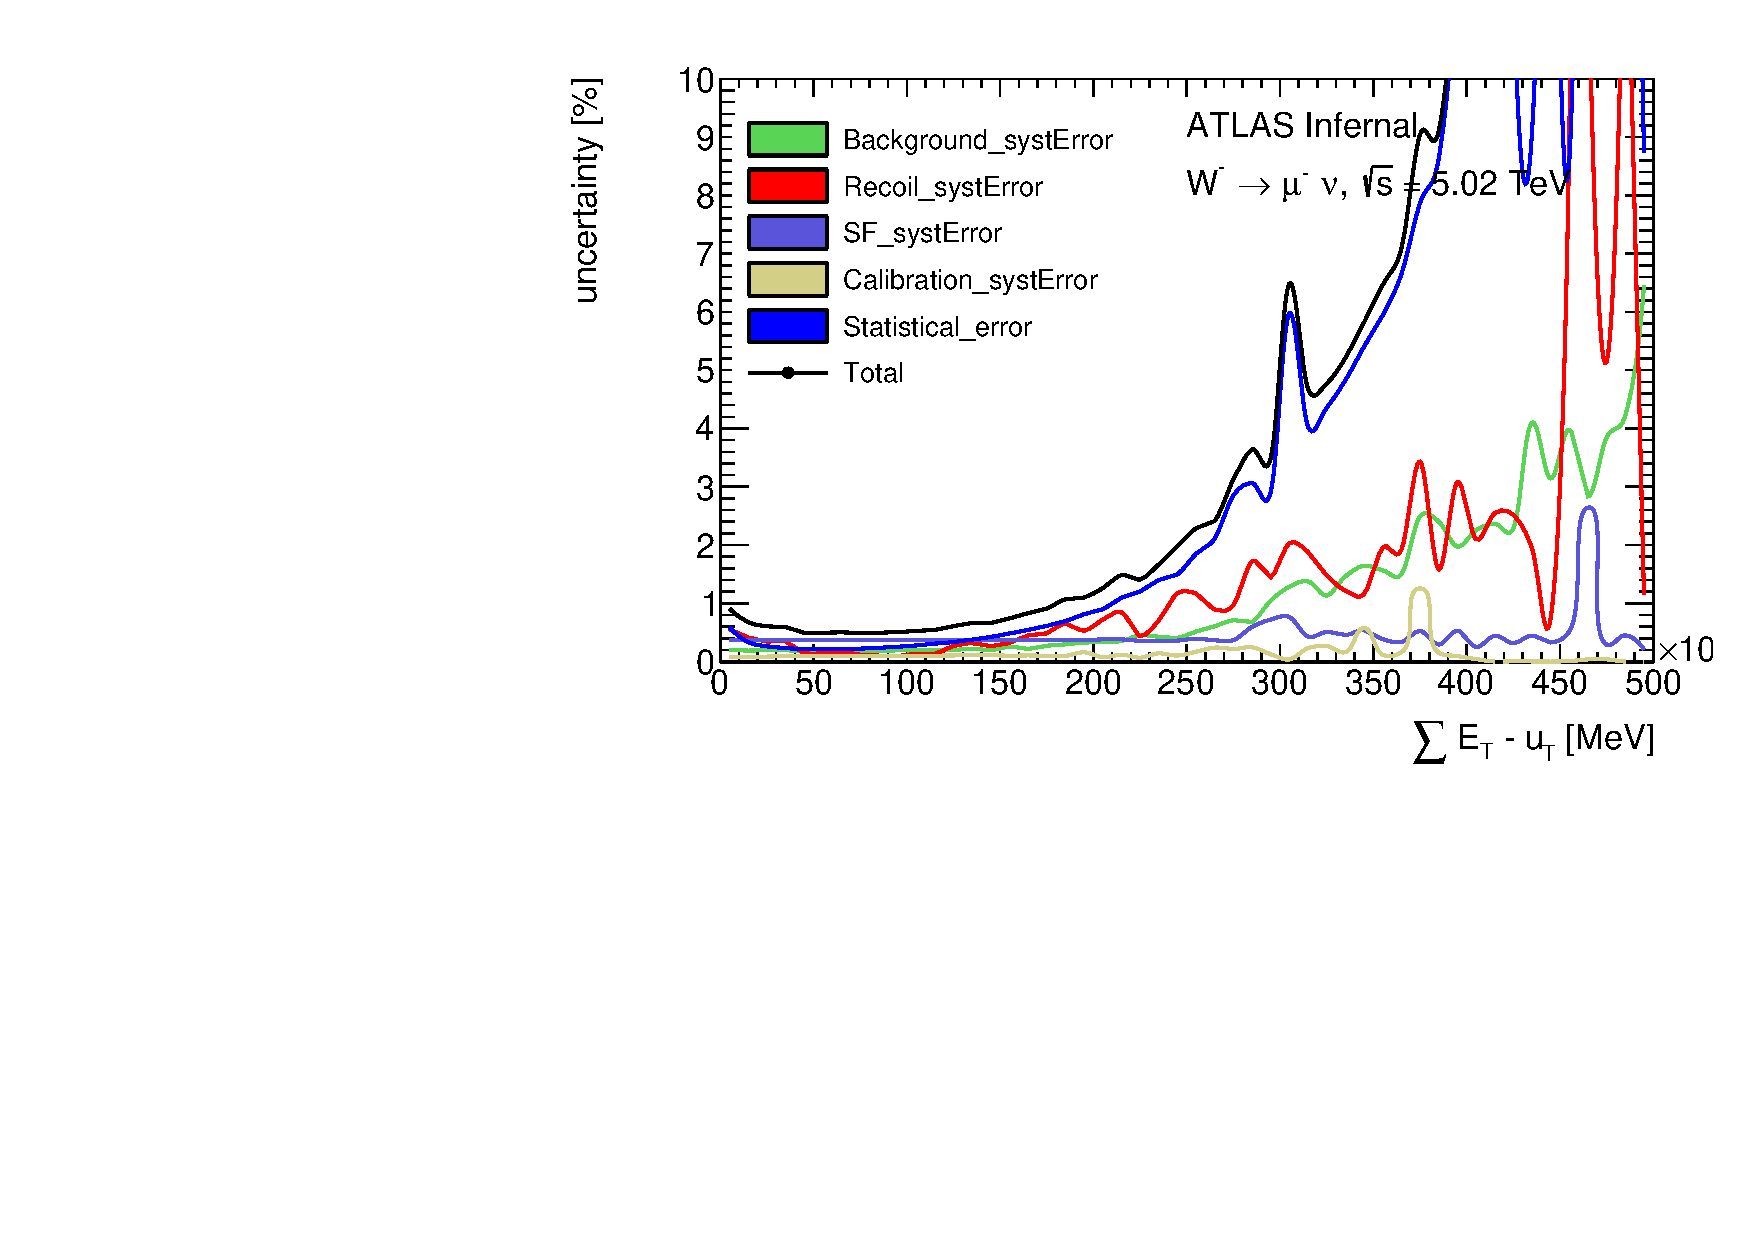
\includegraphics[width=.49\textwidth]{errors_SETUE_cut7_minusmunu_5TeV__NormErr.pdf}\label{f:SETUEmm5}}
	{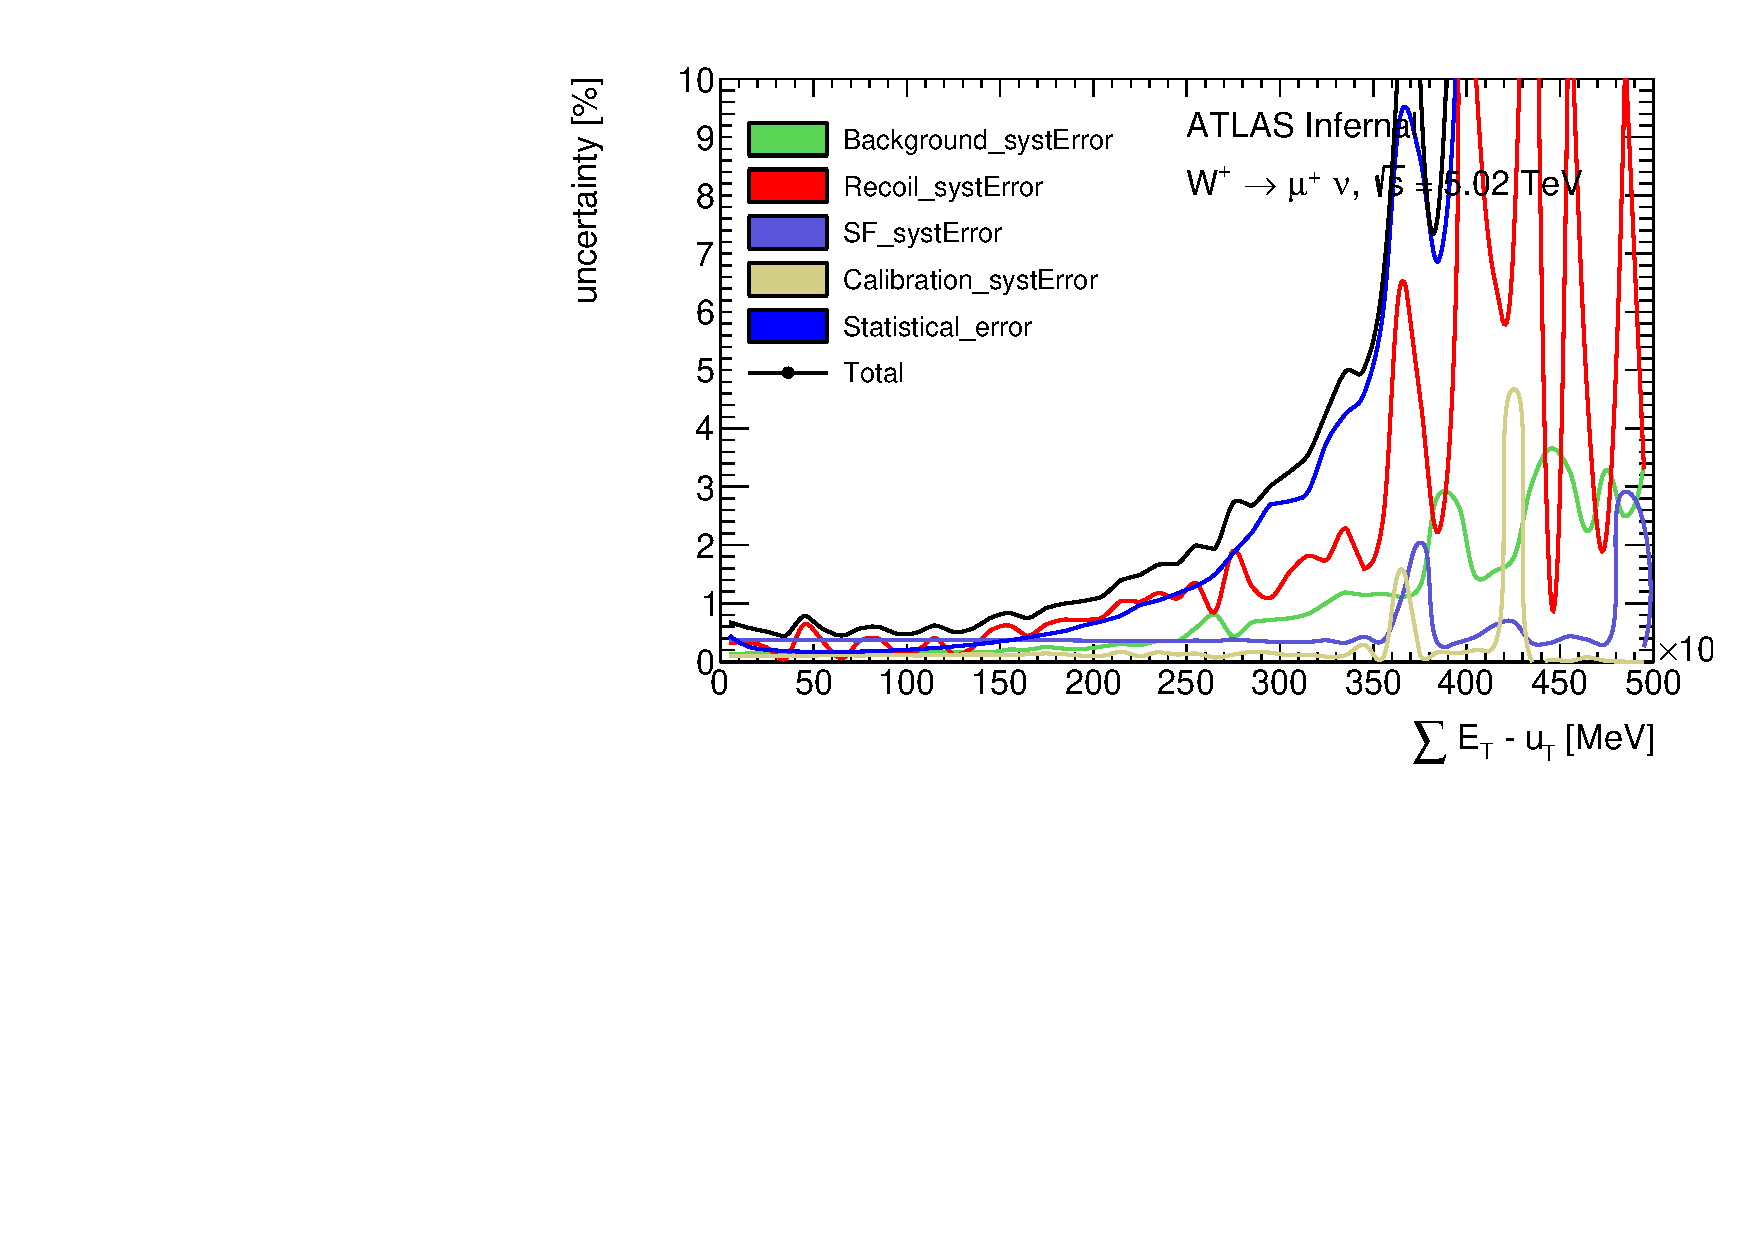
\includegraphics[width=.49\textwidth]{errors_SETUE_cut7_plusmunu_5TeV__NormErr.pdf}\label{f:SETUEpm5}}
	
	{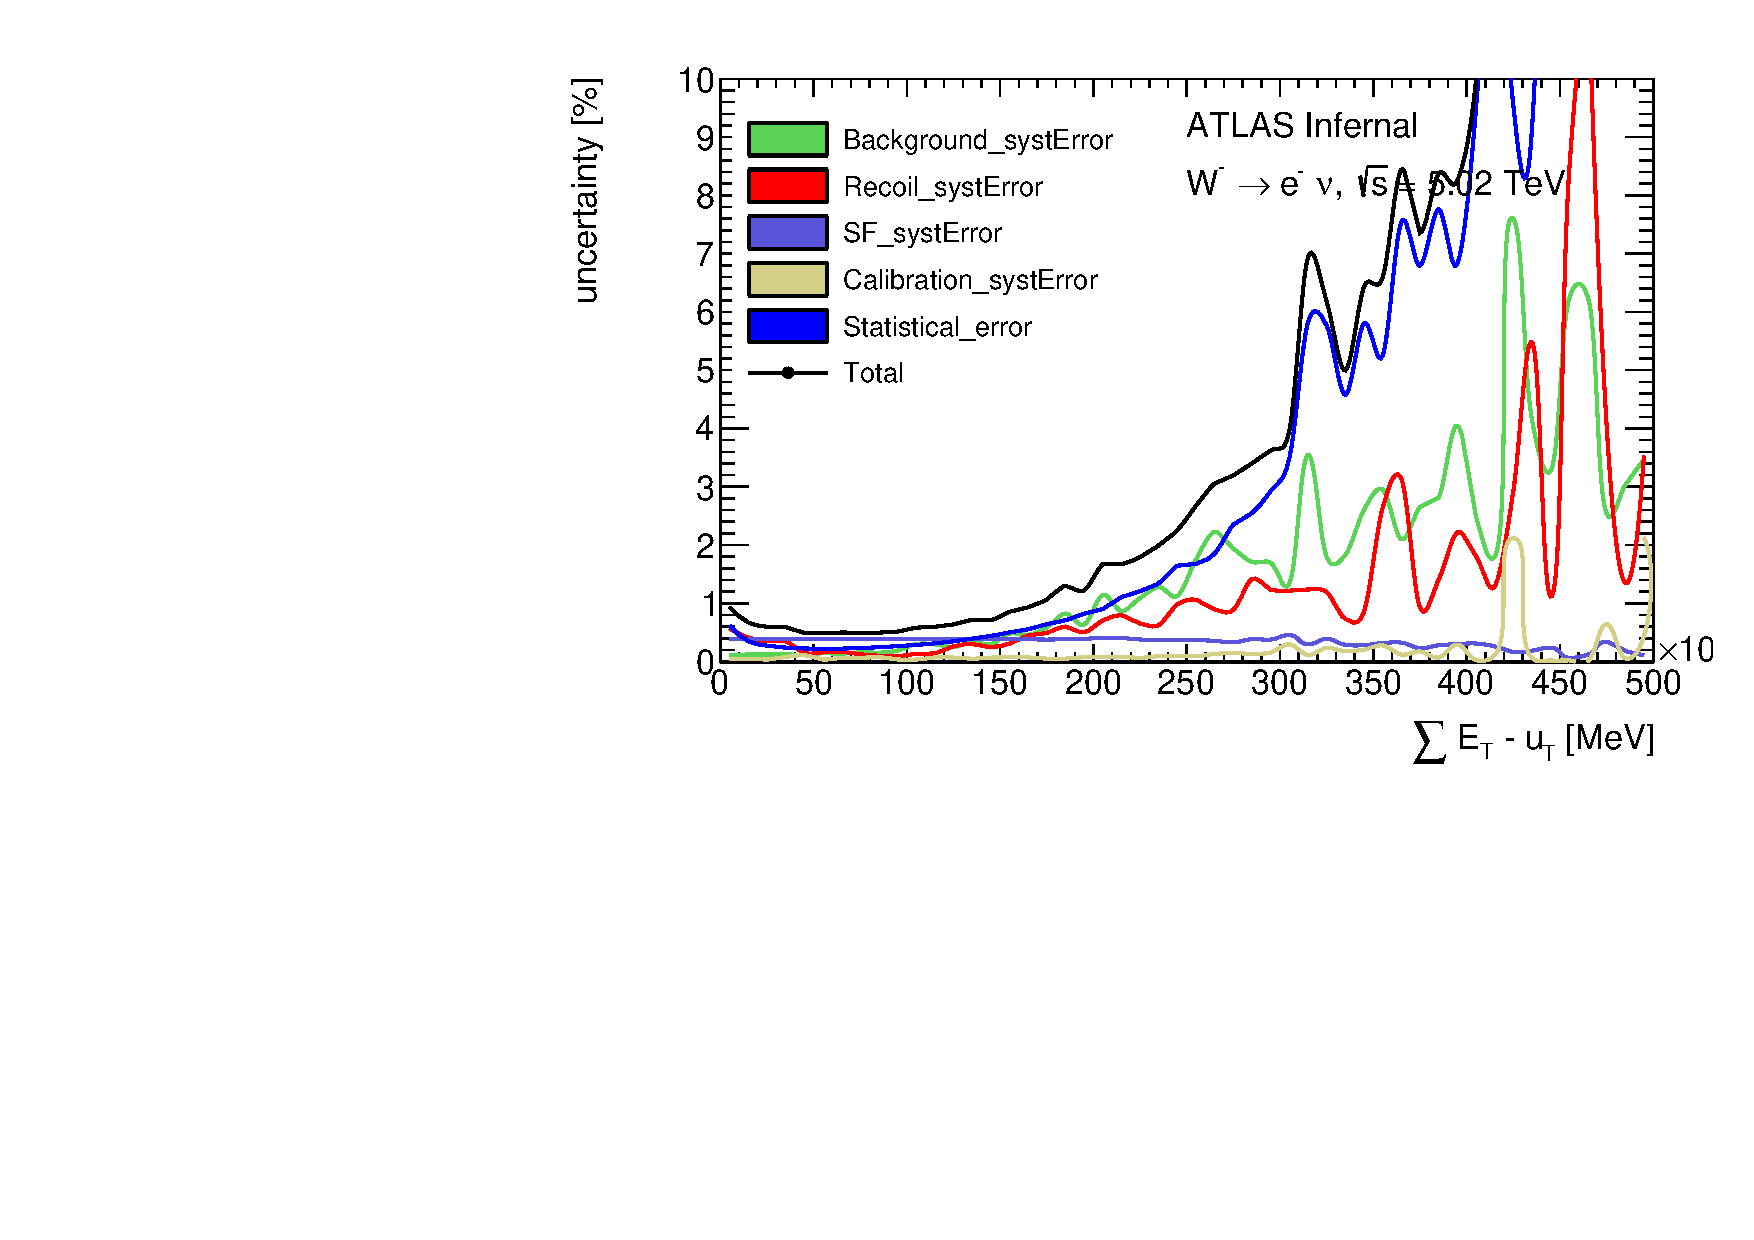
\includegraphics[width=.49\textwidth]{errors_SETUE_cut7_minusenu_5TeV__NormErr.pdf}\label{f:}}
	{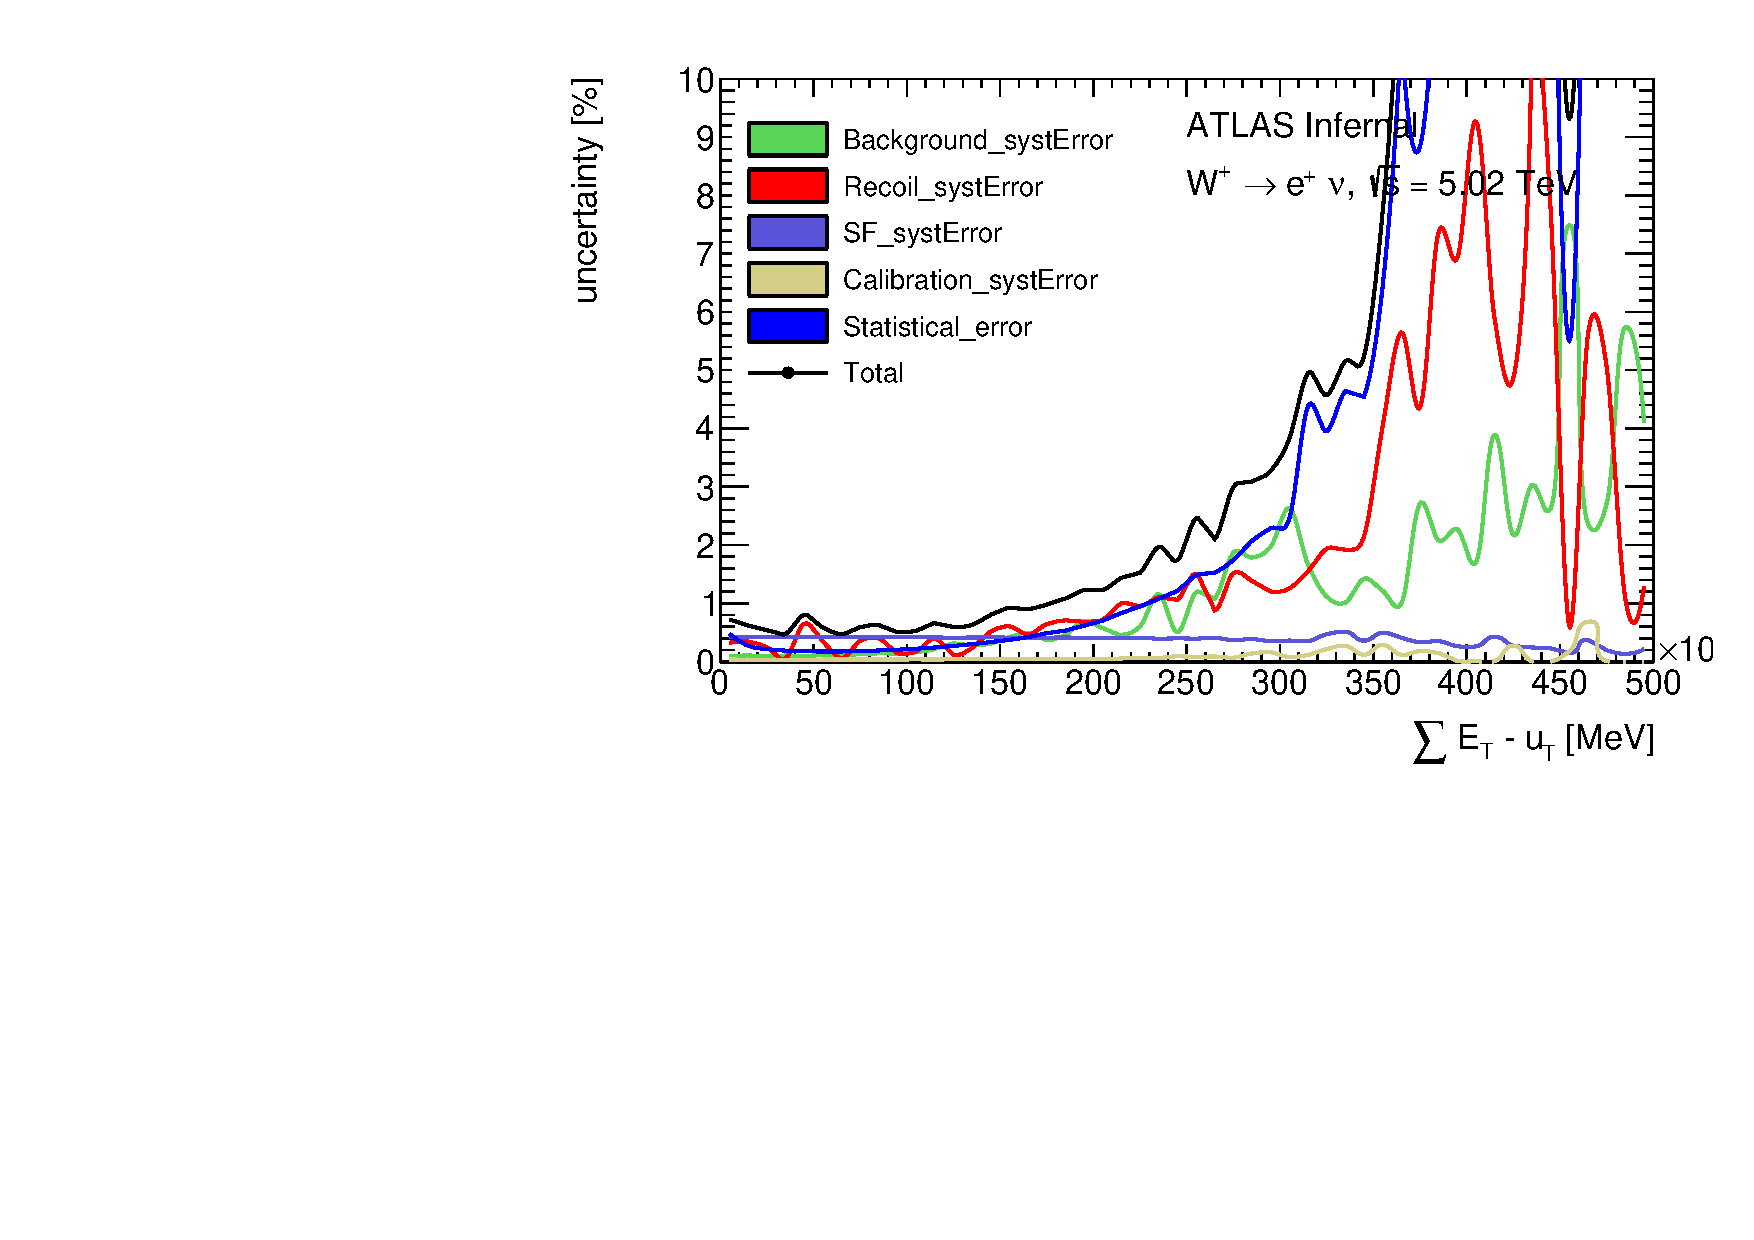
\includegraphics[width=.49\textwidth]{errors_SETUE_cut7_plusenu_5TeV__NormErr.pdf}\label{f:}}
	
	{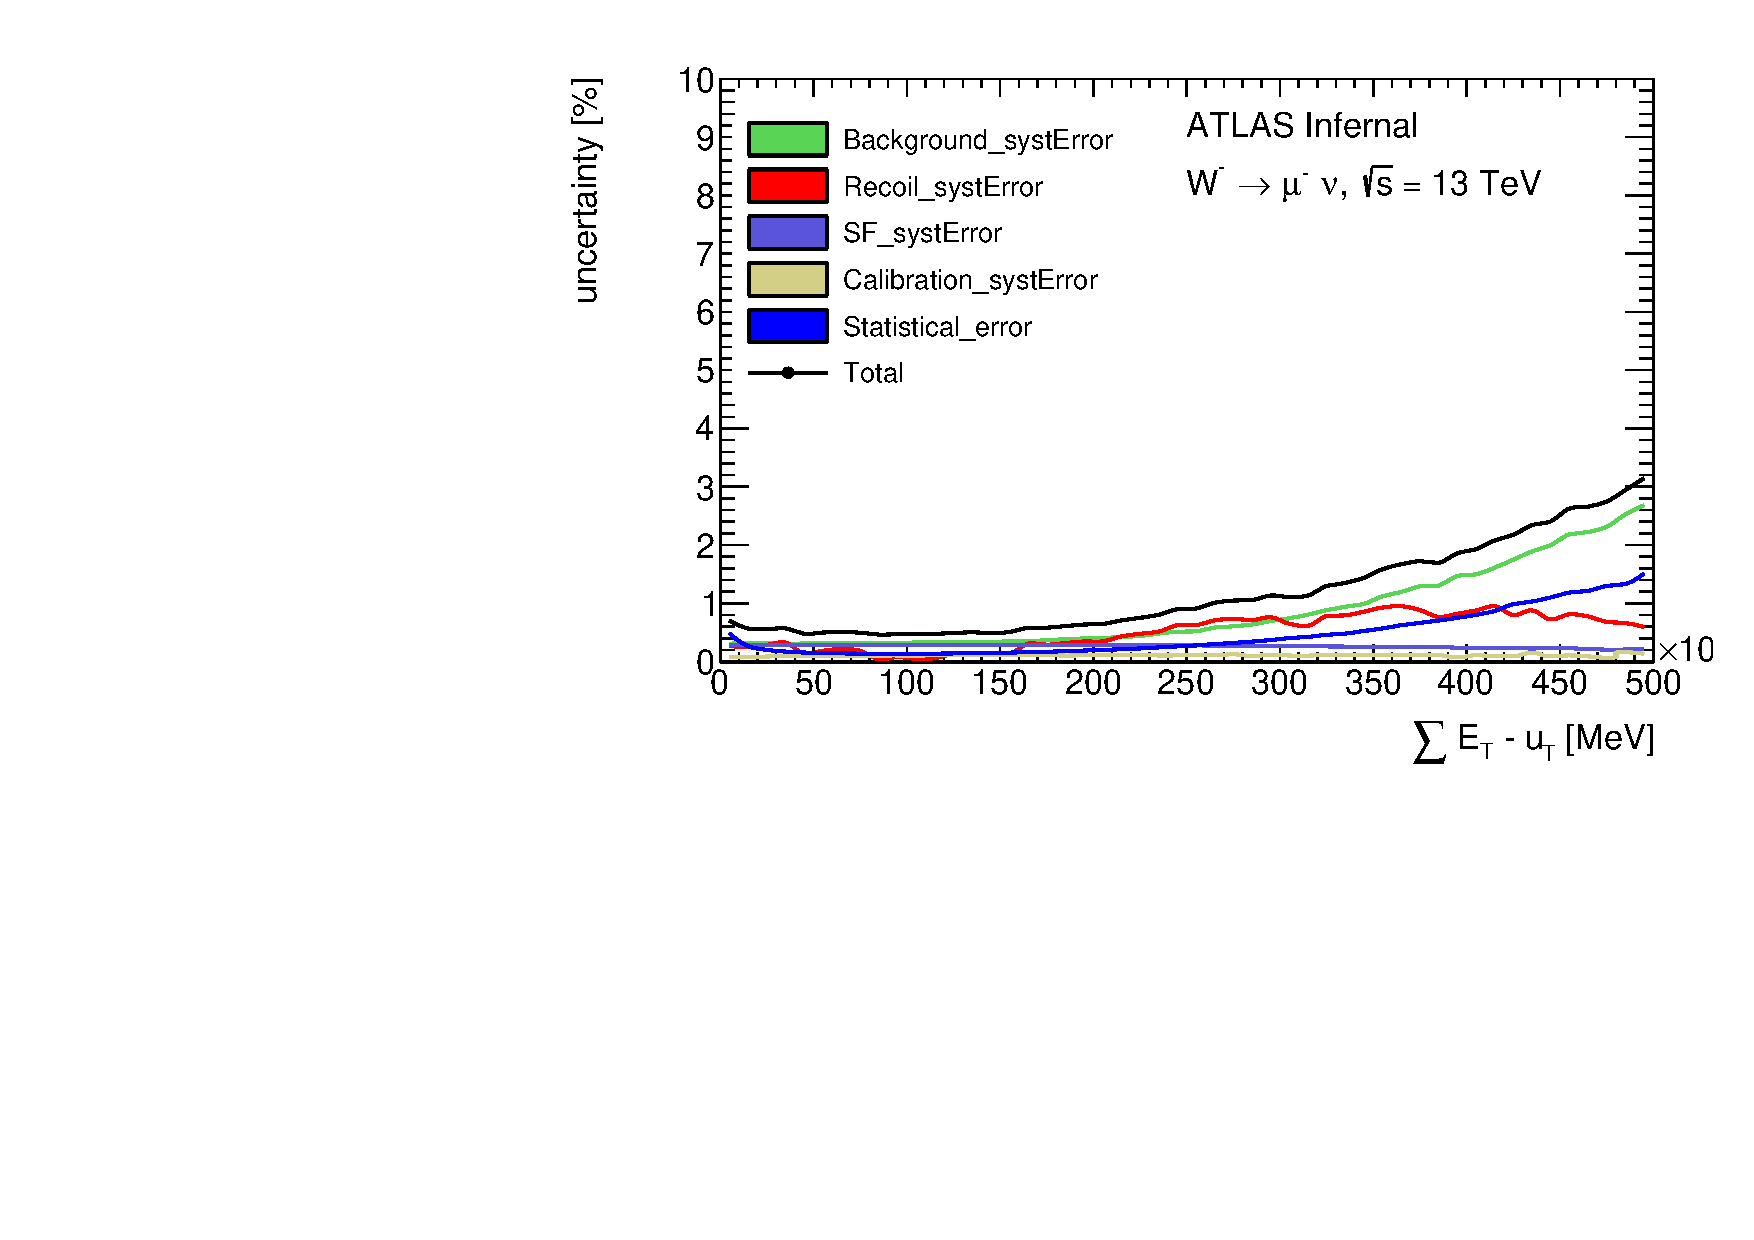
\includegraphics[width=.49\textwidth]{errors_SETUE_cut7_minusmunu_13TeV__NormErr.pdf}\label{f:SETUEmm13}}
	{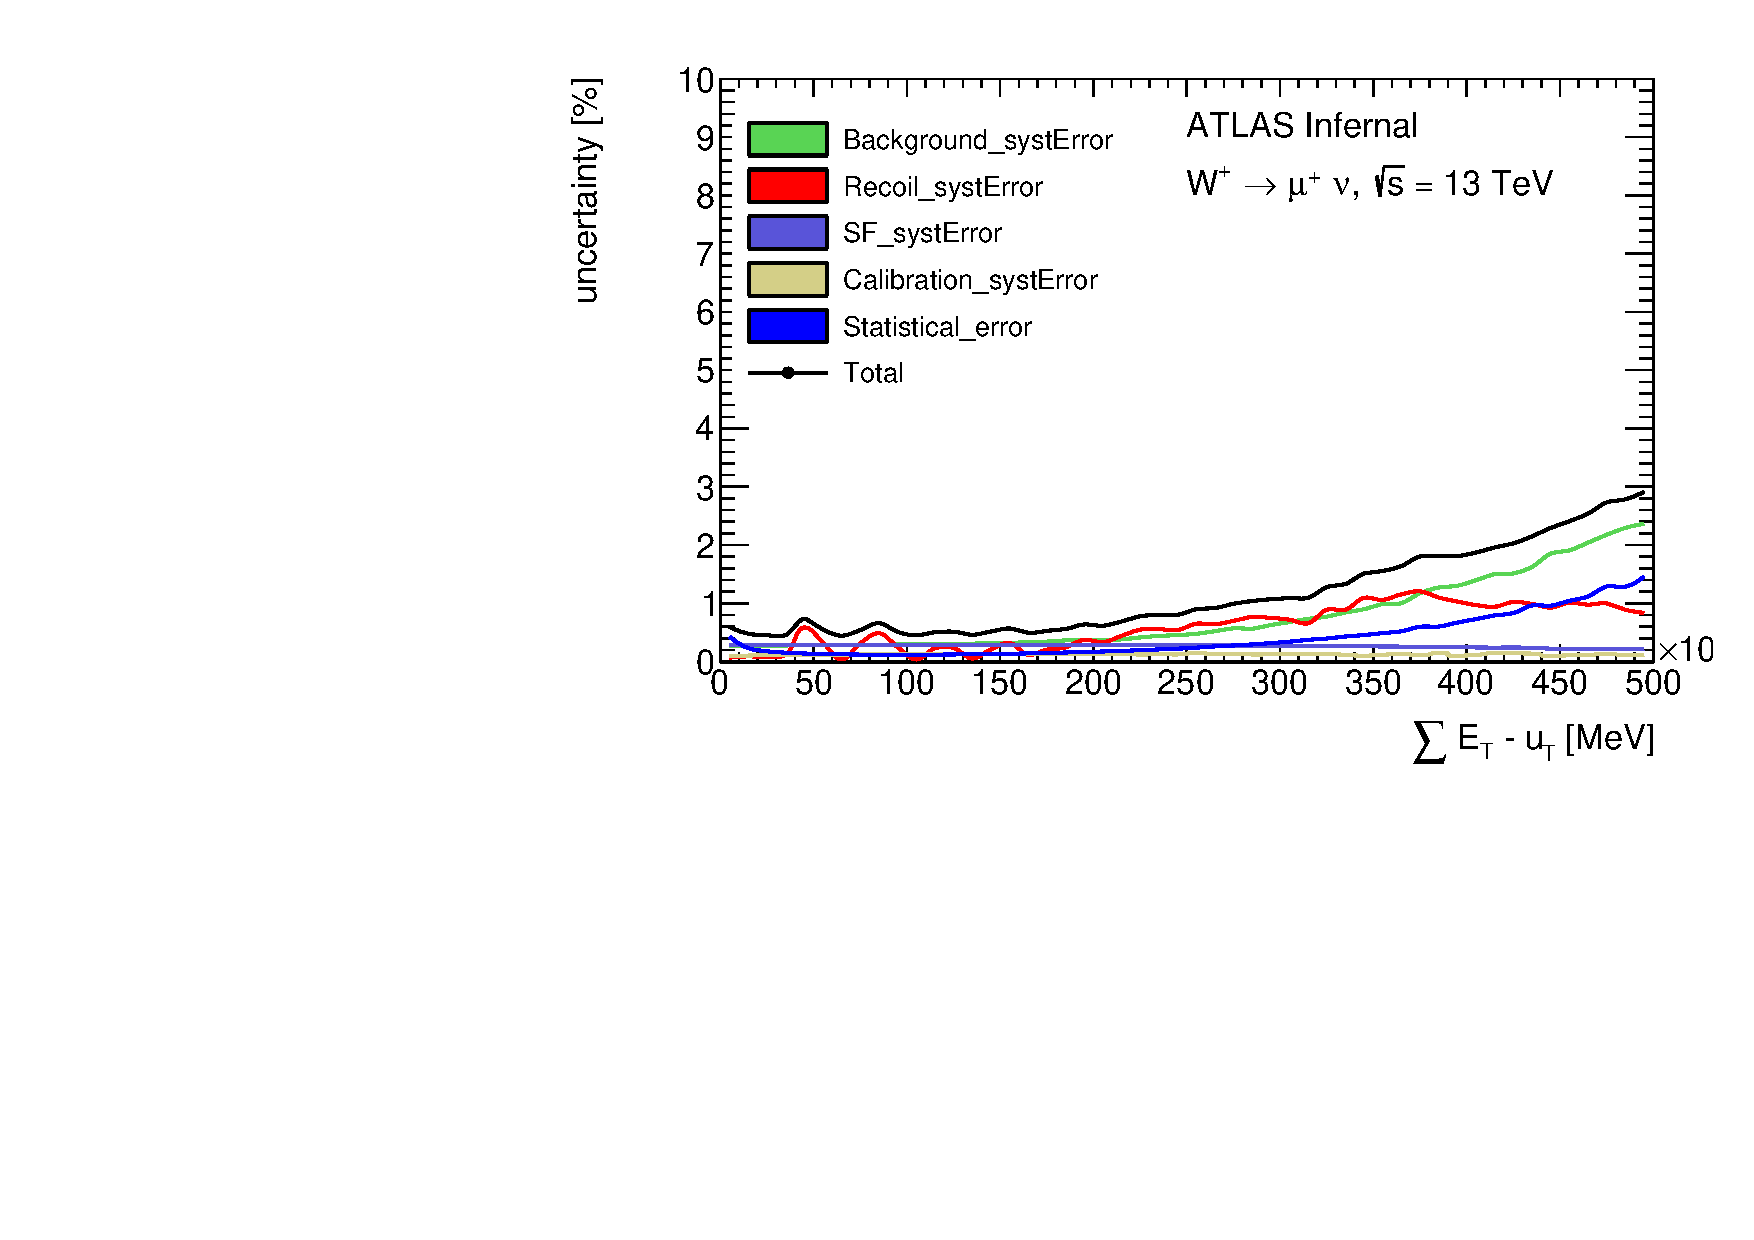
\includegraphics[width=.49\textwidth]{errors_SETUE_cut7_plusmunu_13TeV__NormErr.pdf}\label{f:SETUEpm13}}
	{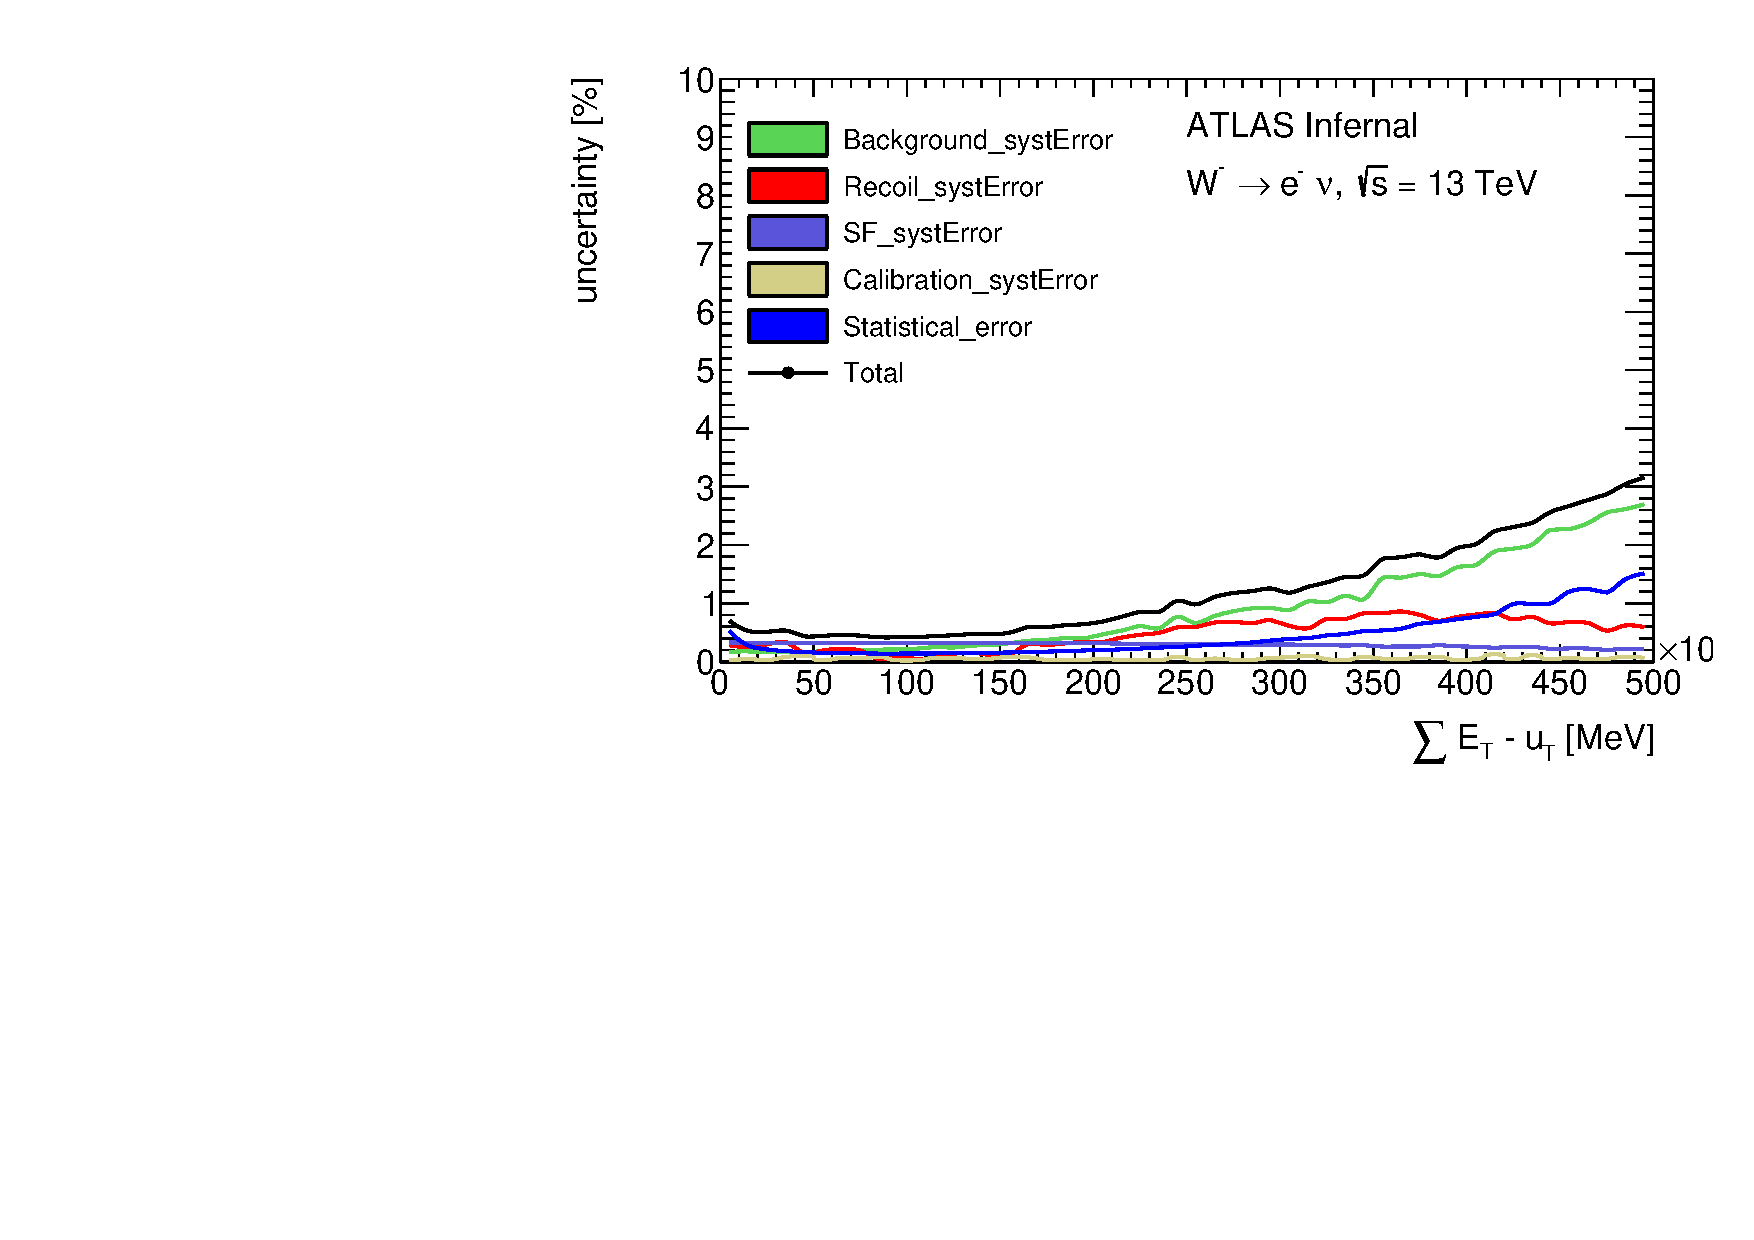
\includegraphics[width=.49\textwidth]{errors_SETUE_cut7_minusenu_13TeV__NormErr.pdf}\label{f:}}
	{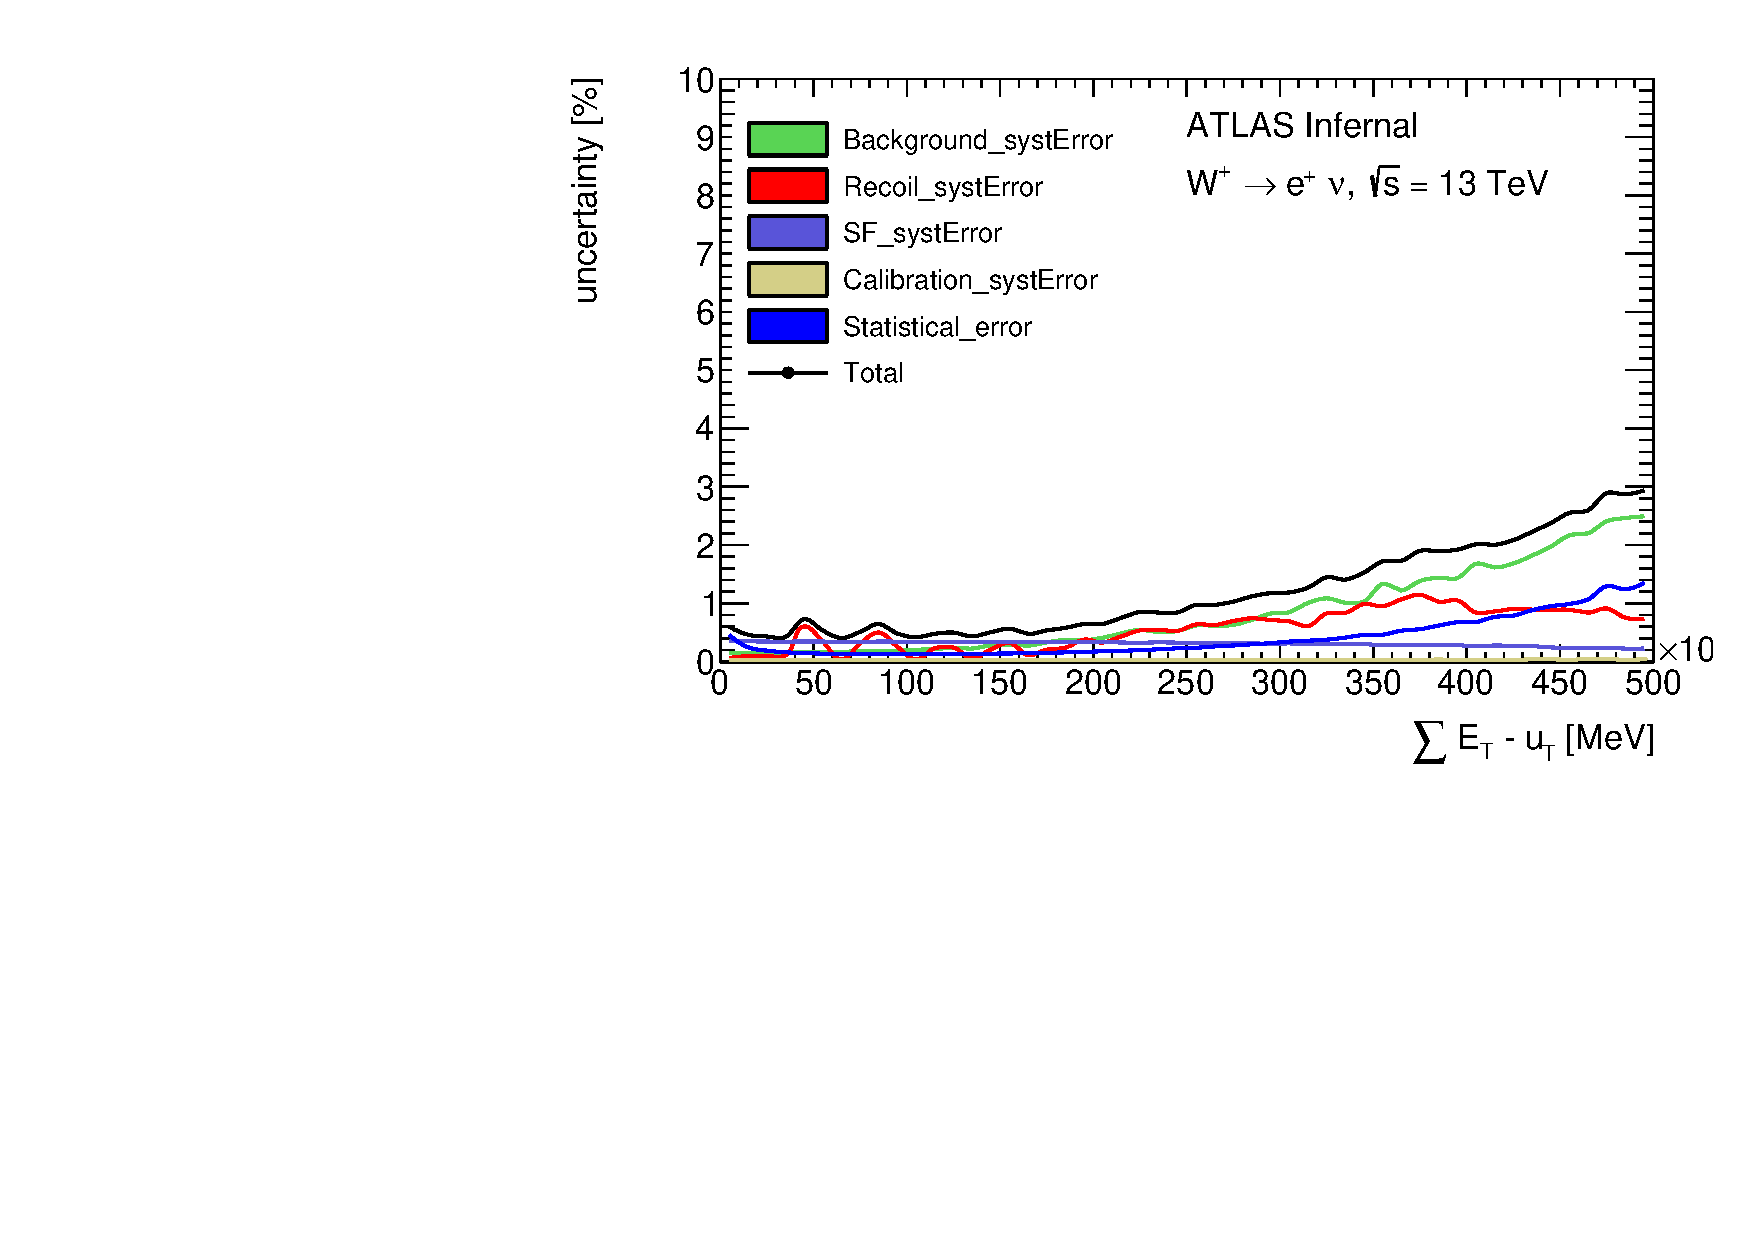
\includegraphics[width=.49\textwidth]{errors_SETUE_cut7_plusenu_13TeV__NormErr.pdf}\label{f:}}
	
	\caption{$\Sigma \bar{E_T}$ systematic error breakdown in the muon and electron channel  for the $\sqrt{s} = 5$~\TeV\ and $\sqrt{s} = 13$~\TeV\ datasets.}
\end{figure}
%

\begin{figure}[h]
	\centering
	{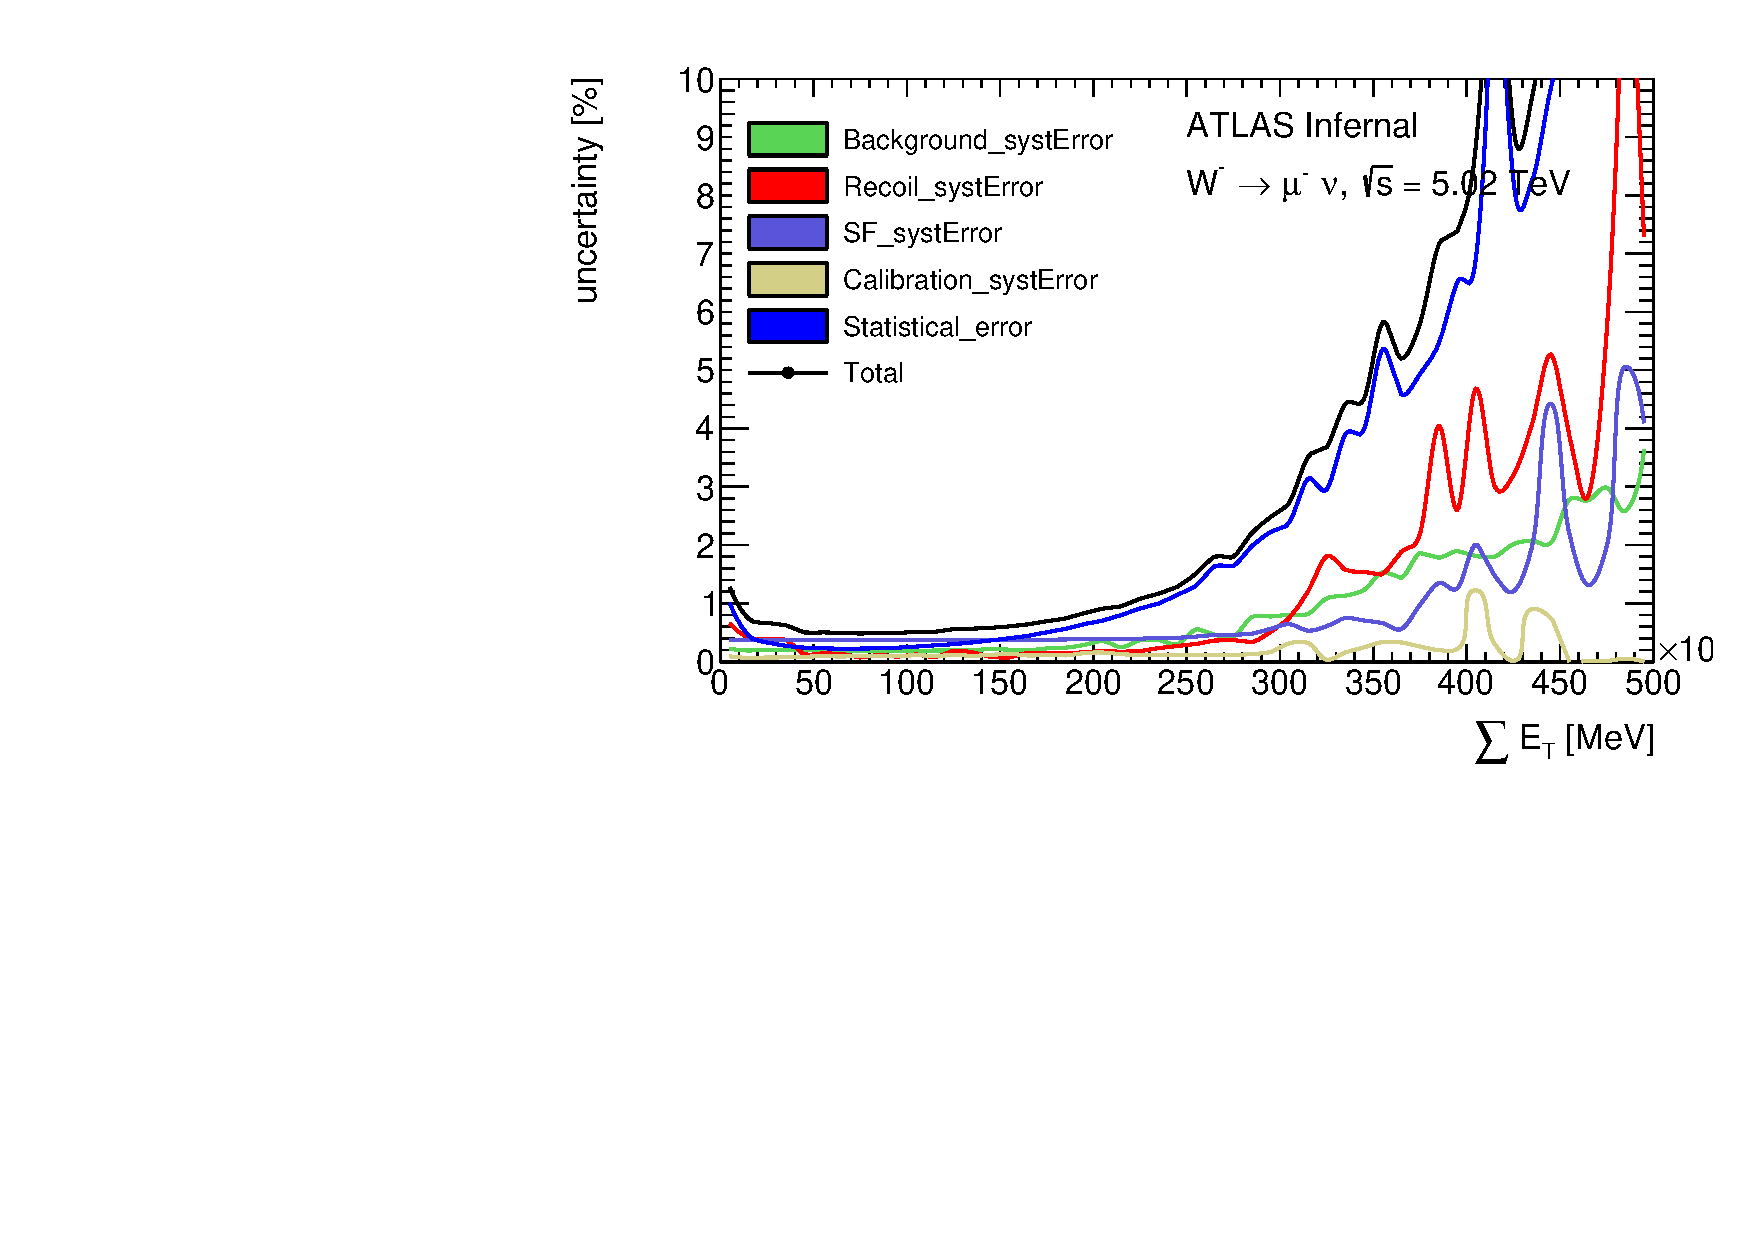
\includegraphics[width=.49\textwidth]{errors_SET_cut7_minusmunu_5TeV__NormErr.pdf}\label{f:set5}}
	{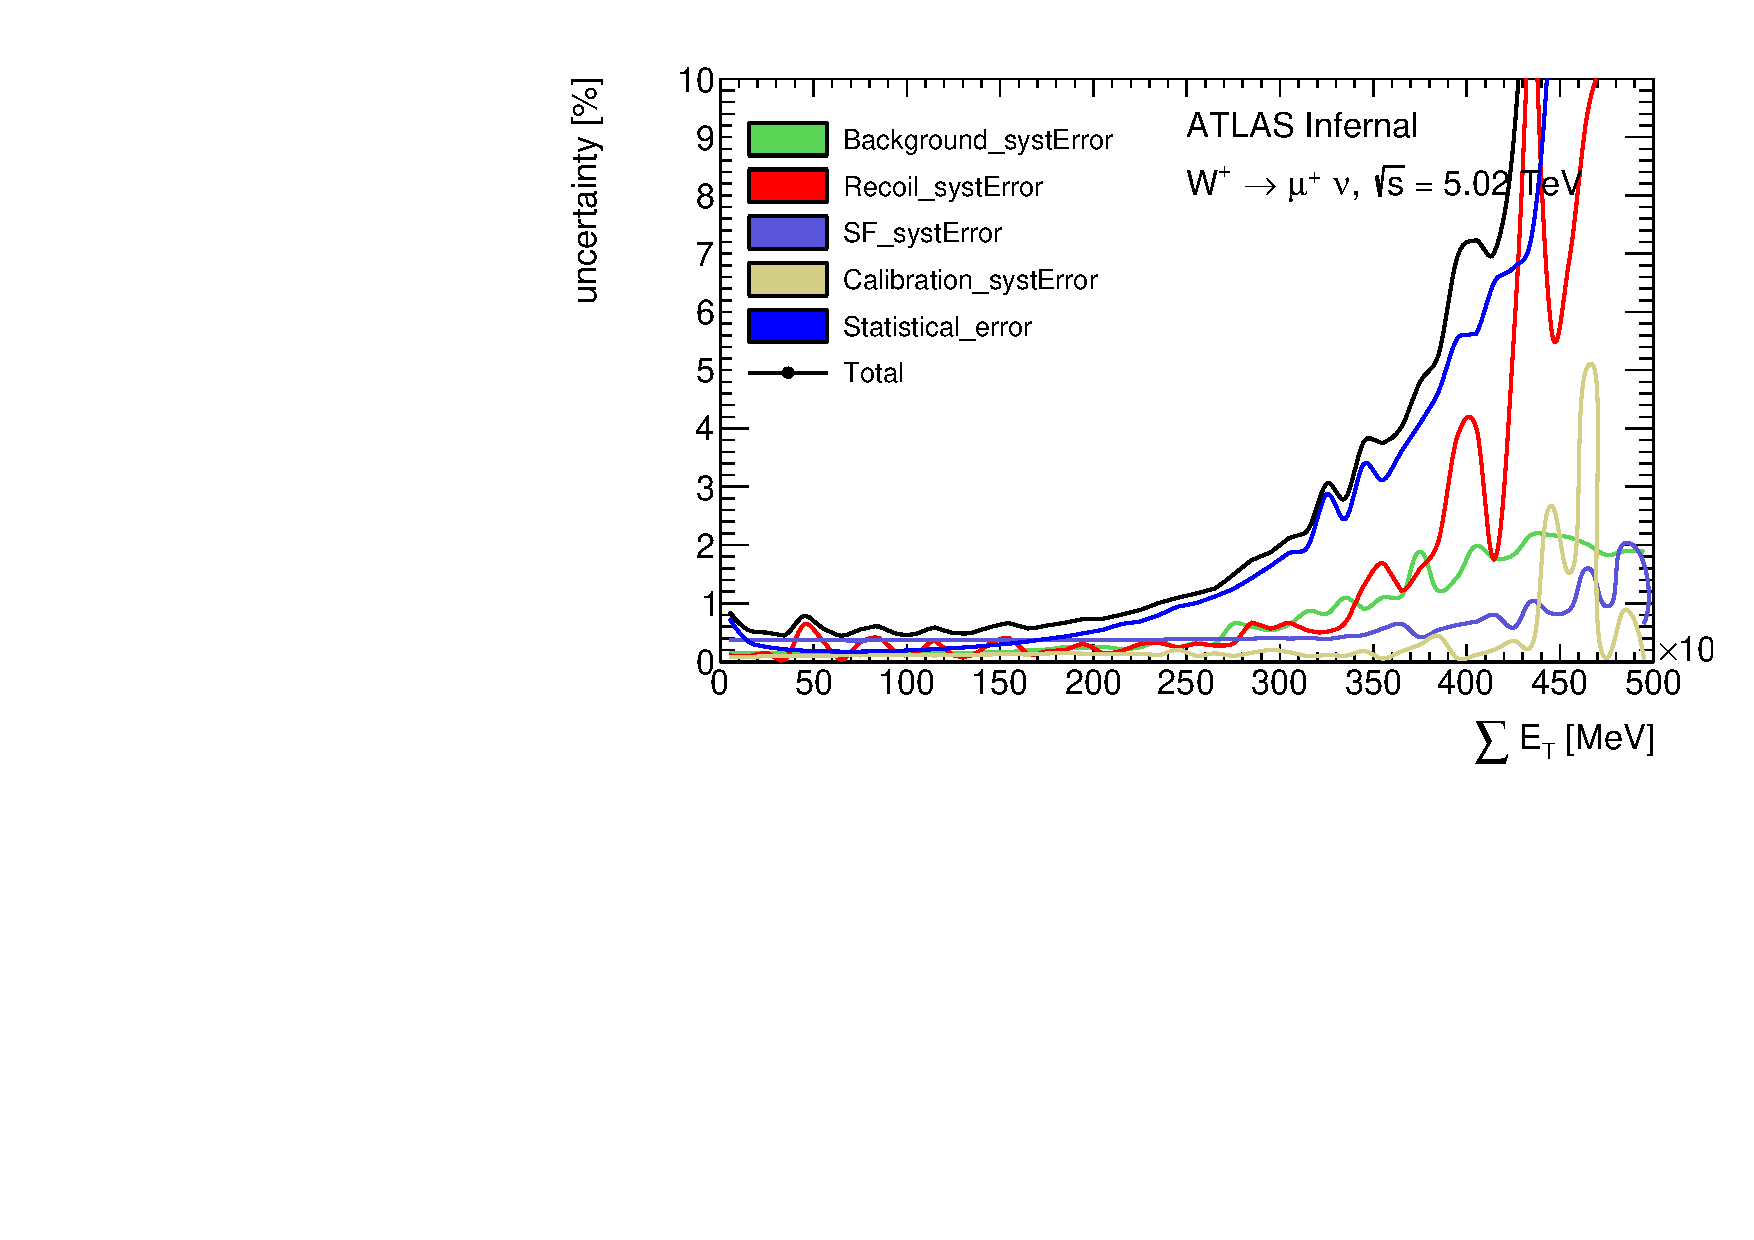
\includegraphics[width=.49\textwidth]{errors_SET_cut7_plusmunu_5TeV__NormErr.pdf}\label{f:setpl}}
	
	{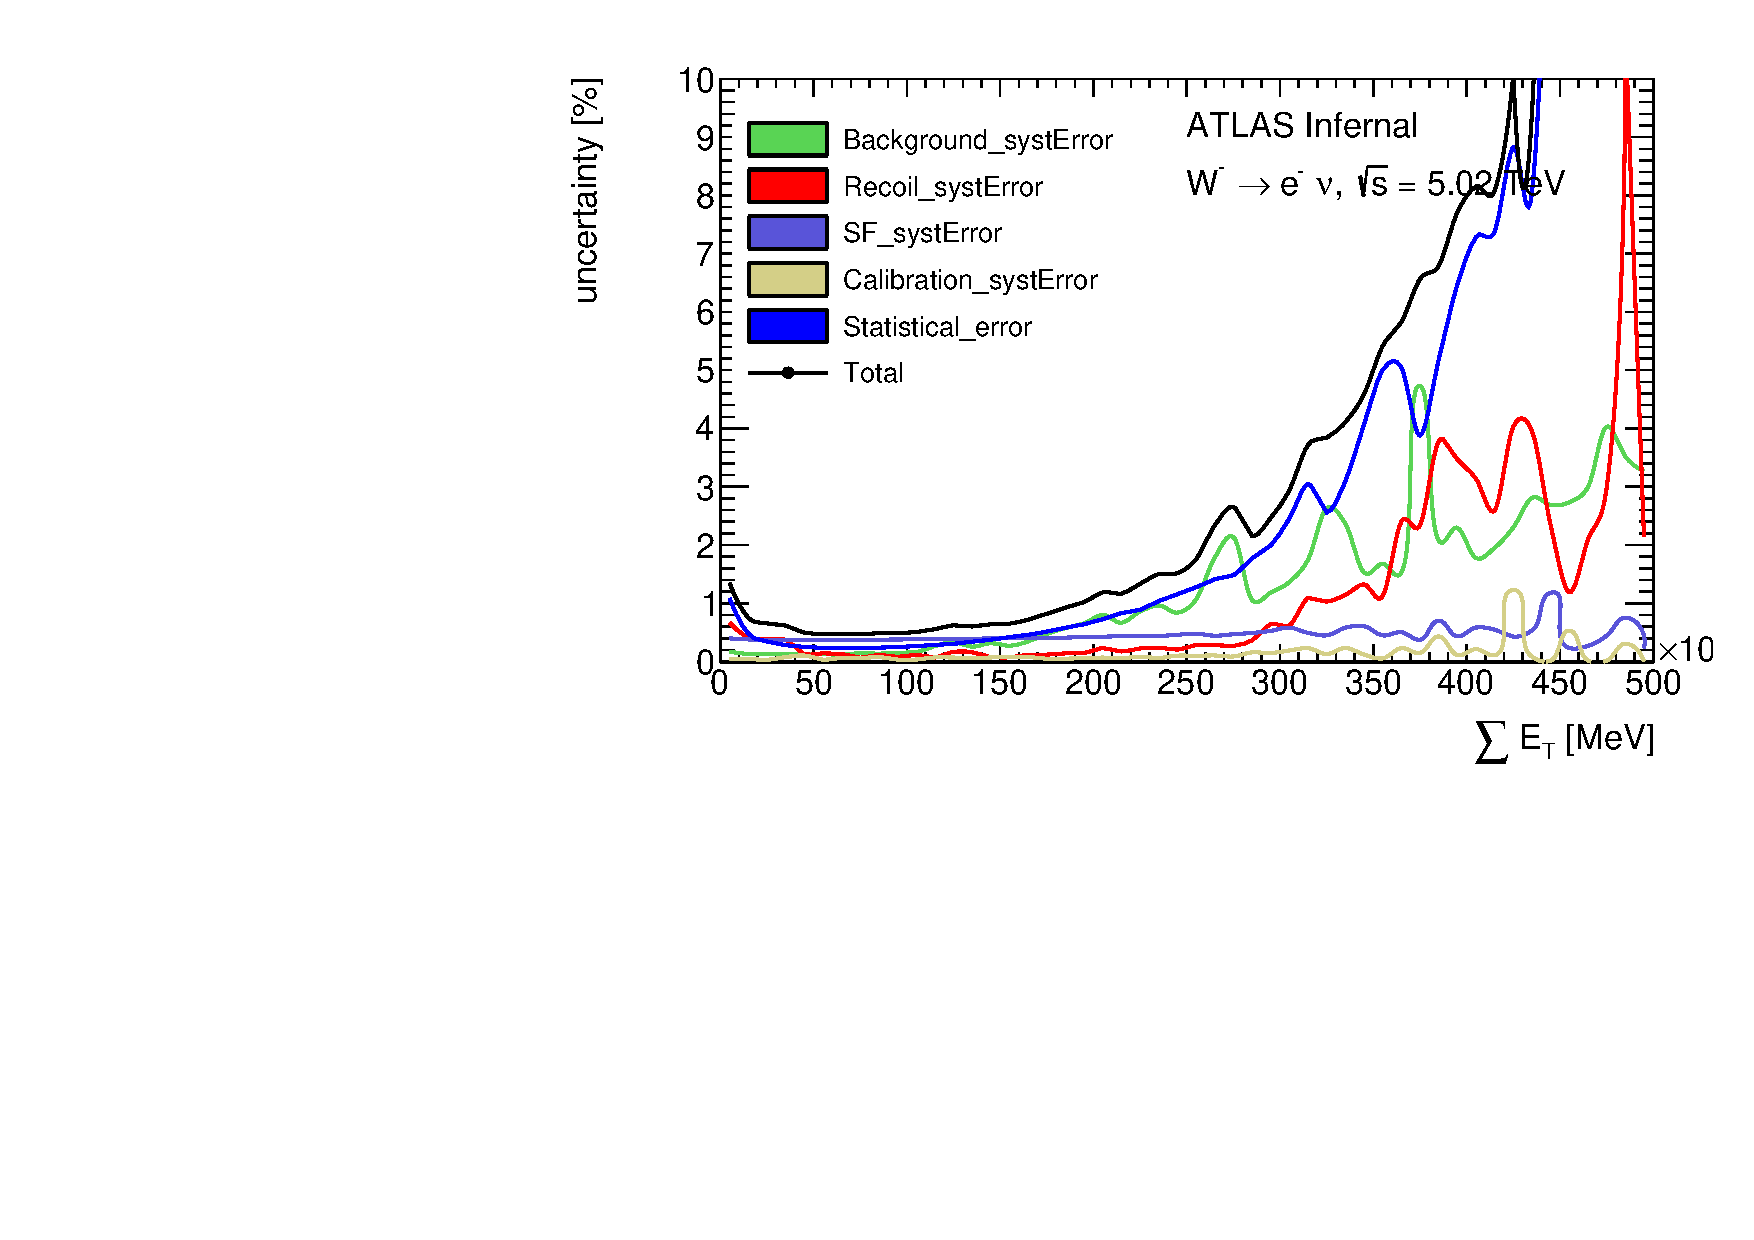
\includegraphics[width=.49\textwidth]{errors_SET_cut7_minusenu_5TeV__NormErr.pdf}\label{f:}}
	{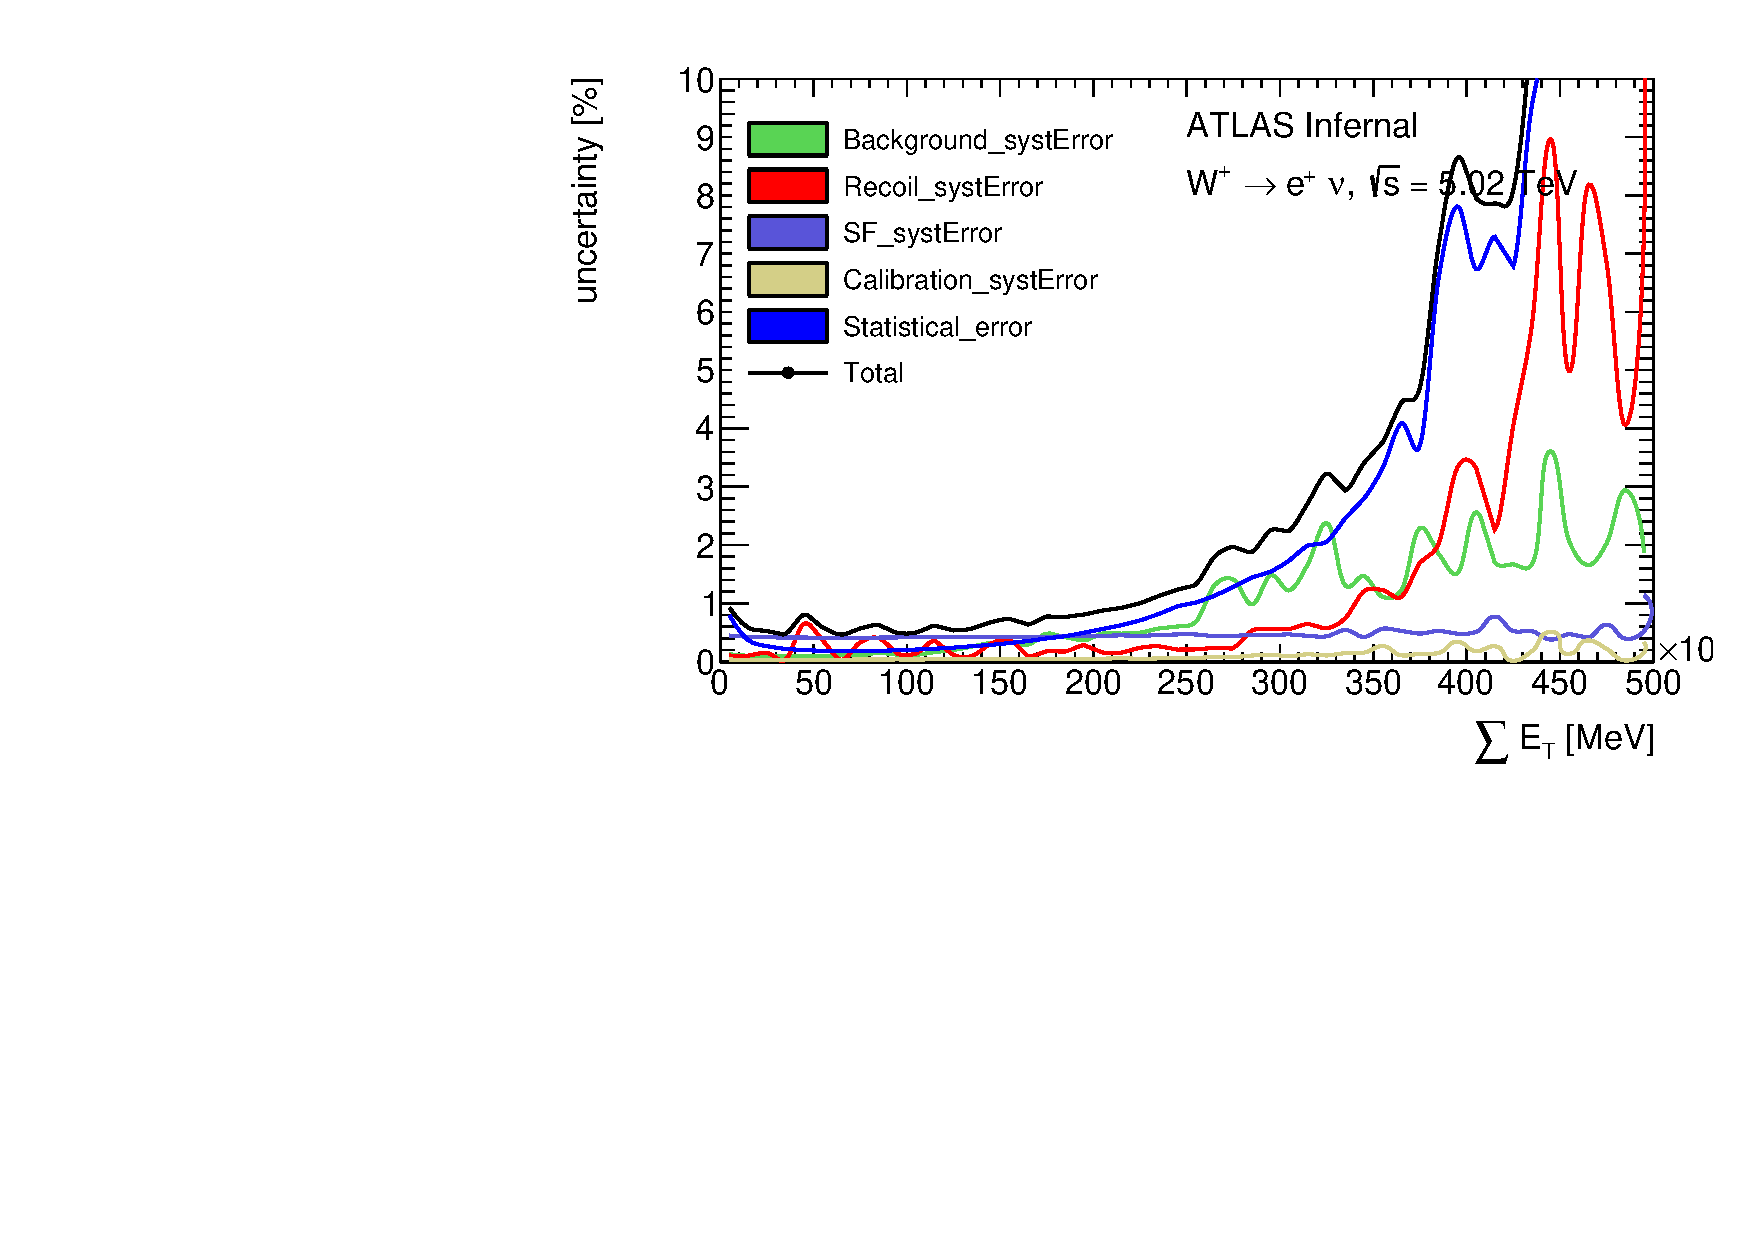
\includegraphics[width=.49\textwidth]{errors_SET_cut7_plusenu_5TeV__NormErr.pdf}\label{f:}}
	
	{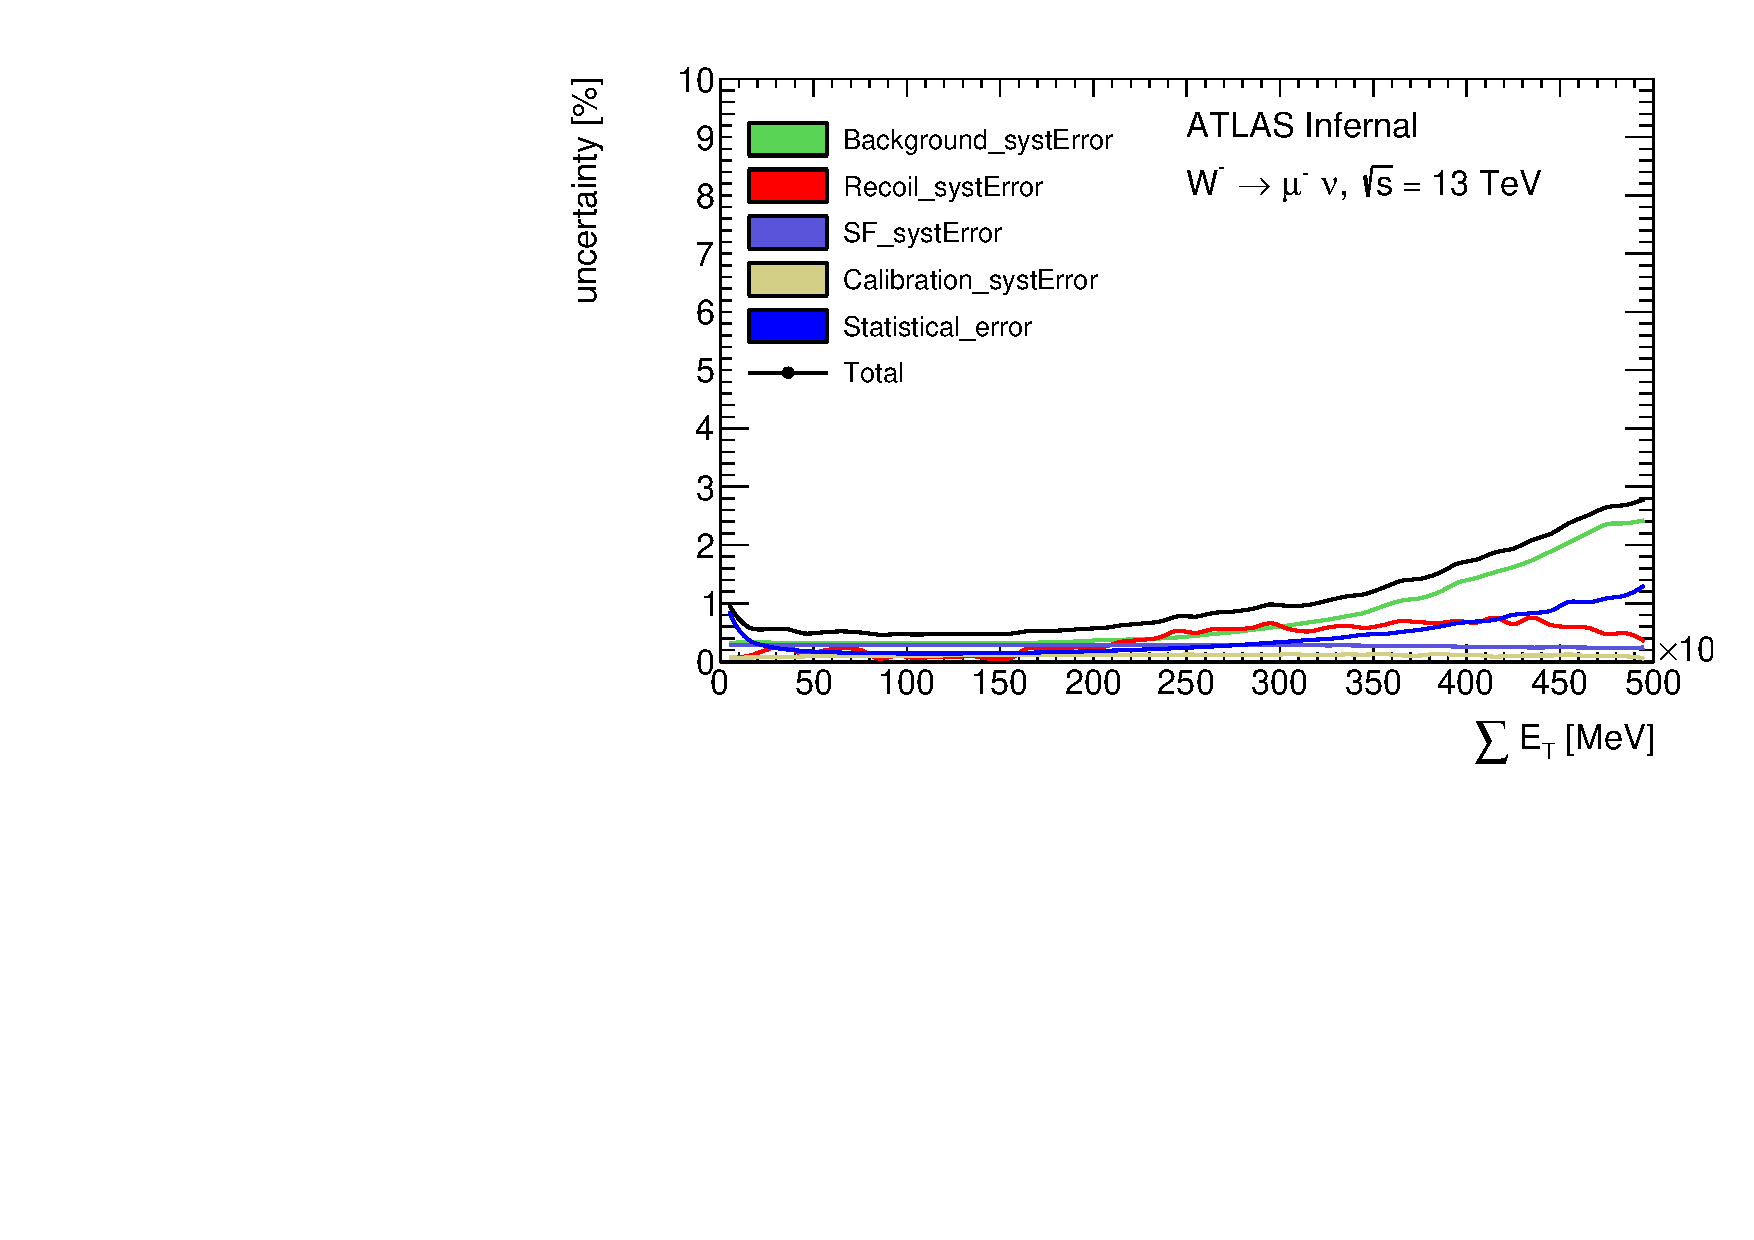
\includegraphics[width=.49\textwidth]{errors_SET_cut7_minusmunu_13TeV__NormErr.pdf}\label{f:set13}}
	{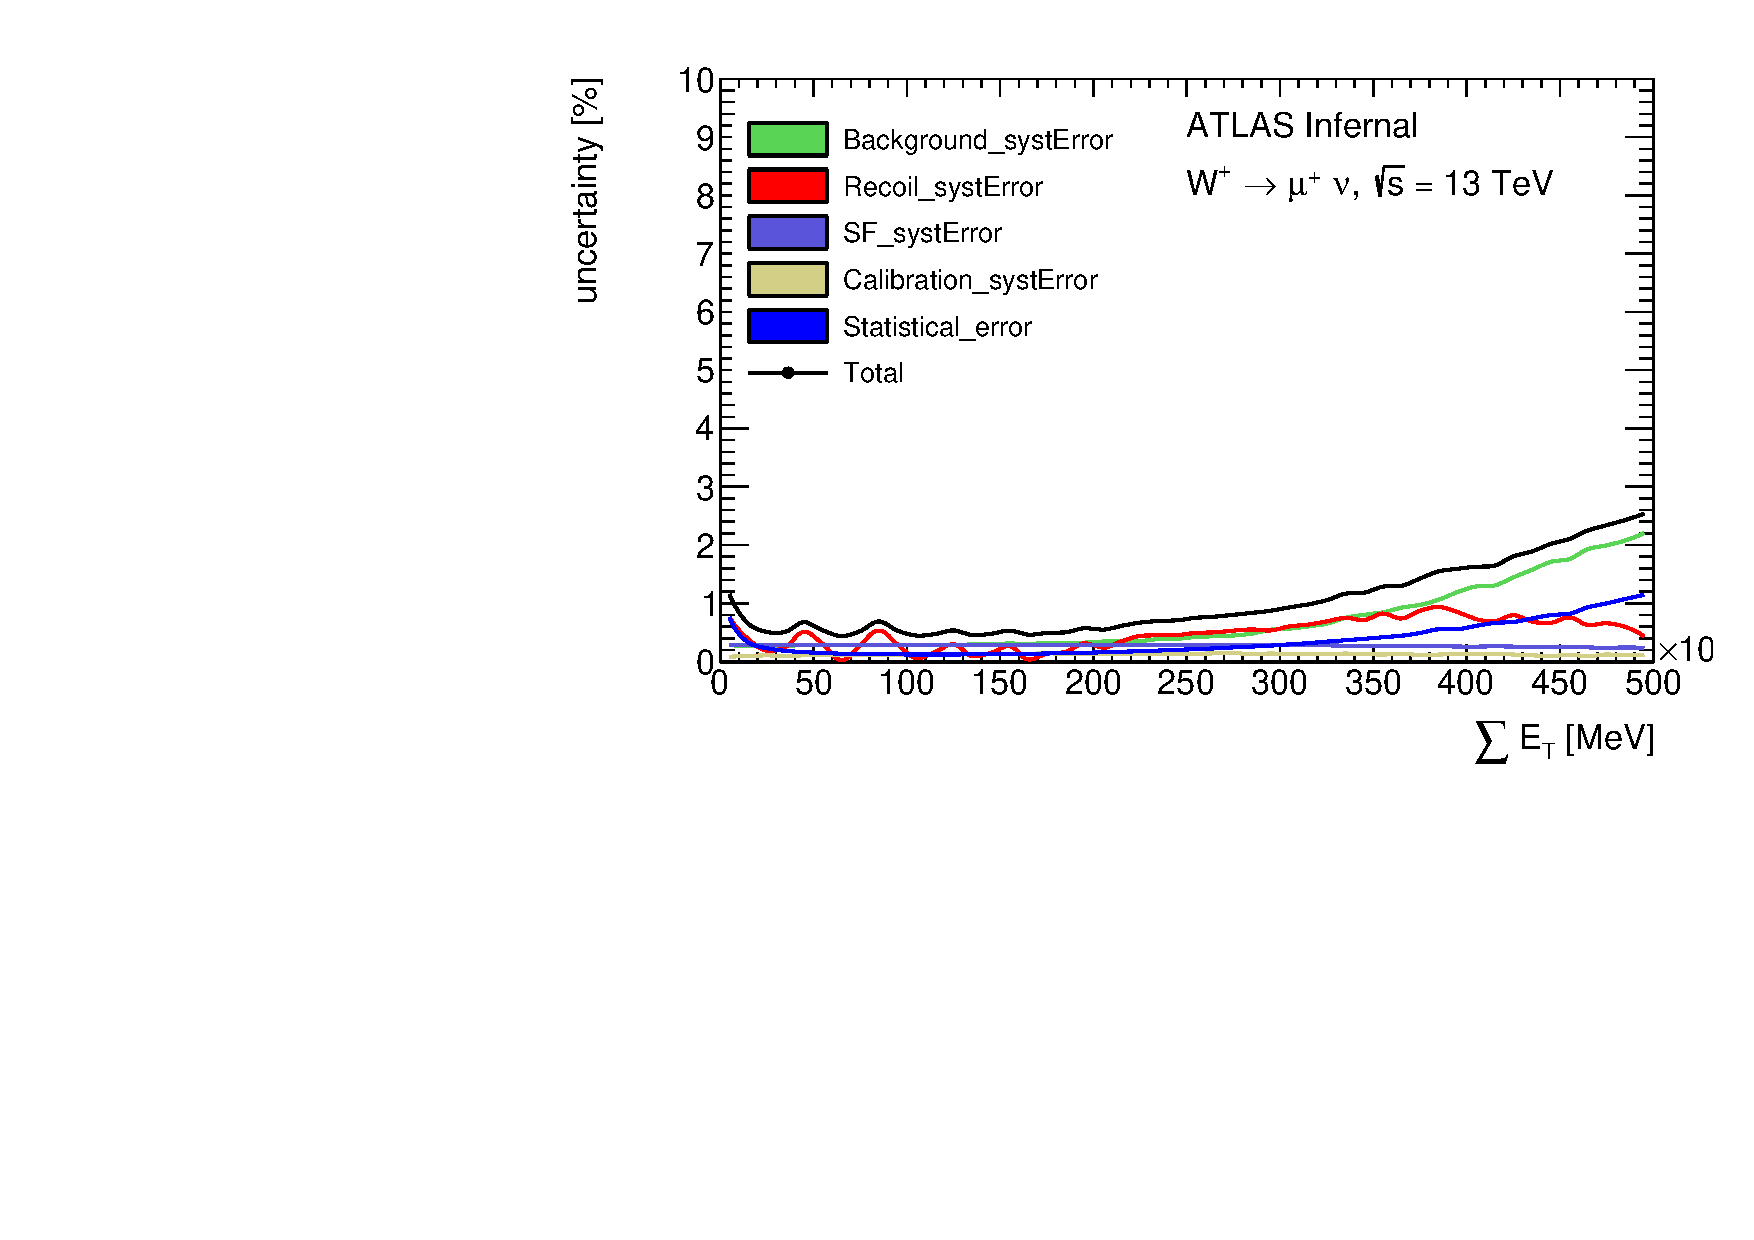
\includegraphics[width=.49\textwidth]{errors_SET_cut7_plusmunu_13TeV__NormErr.pdf}\label{f:setpl13}}
	
	{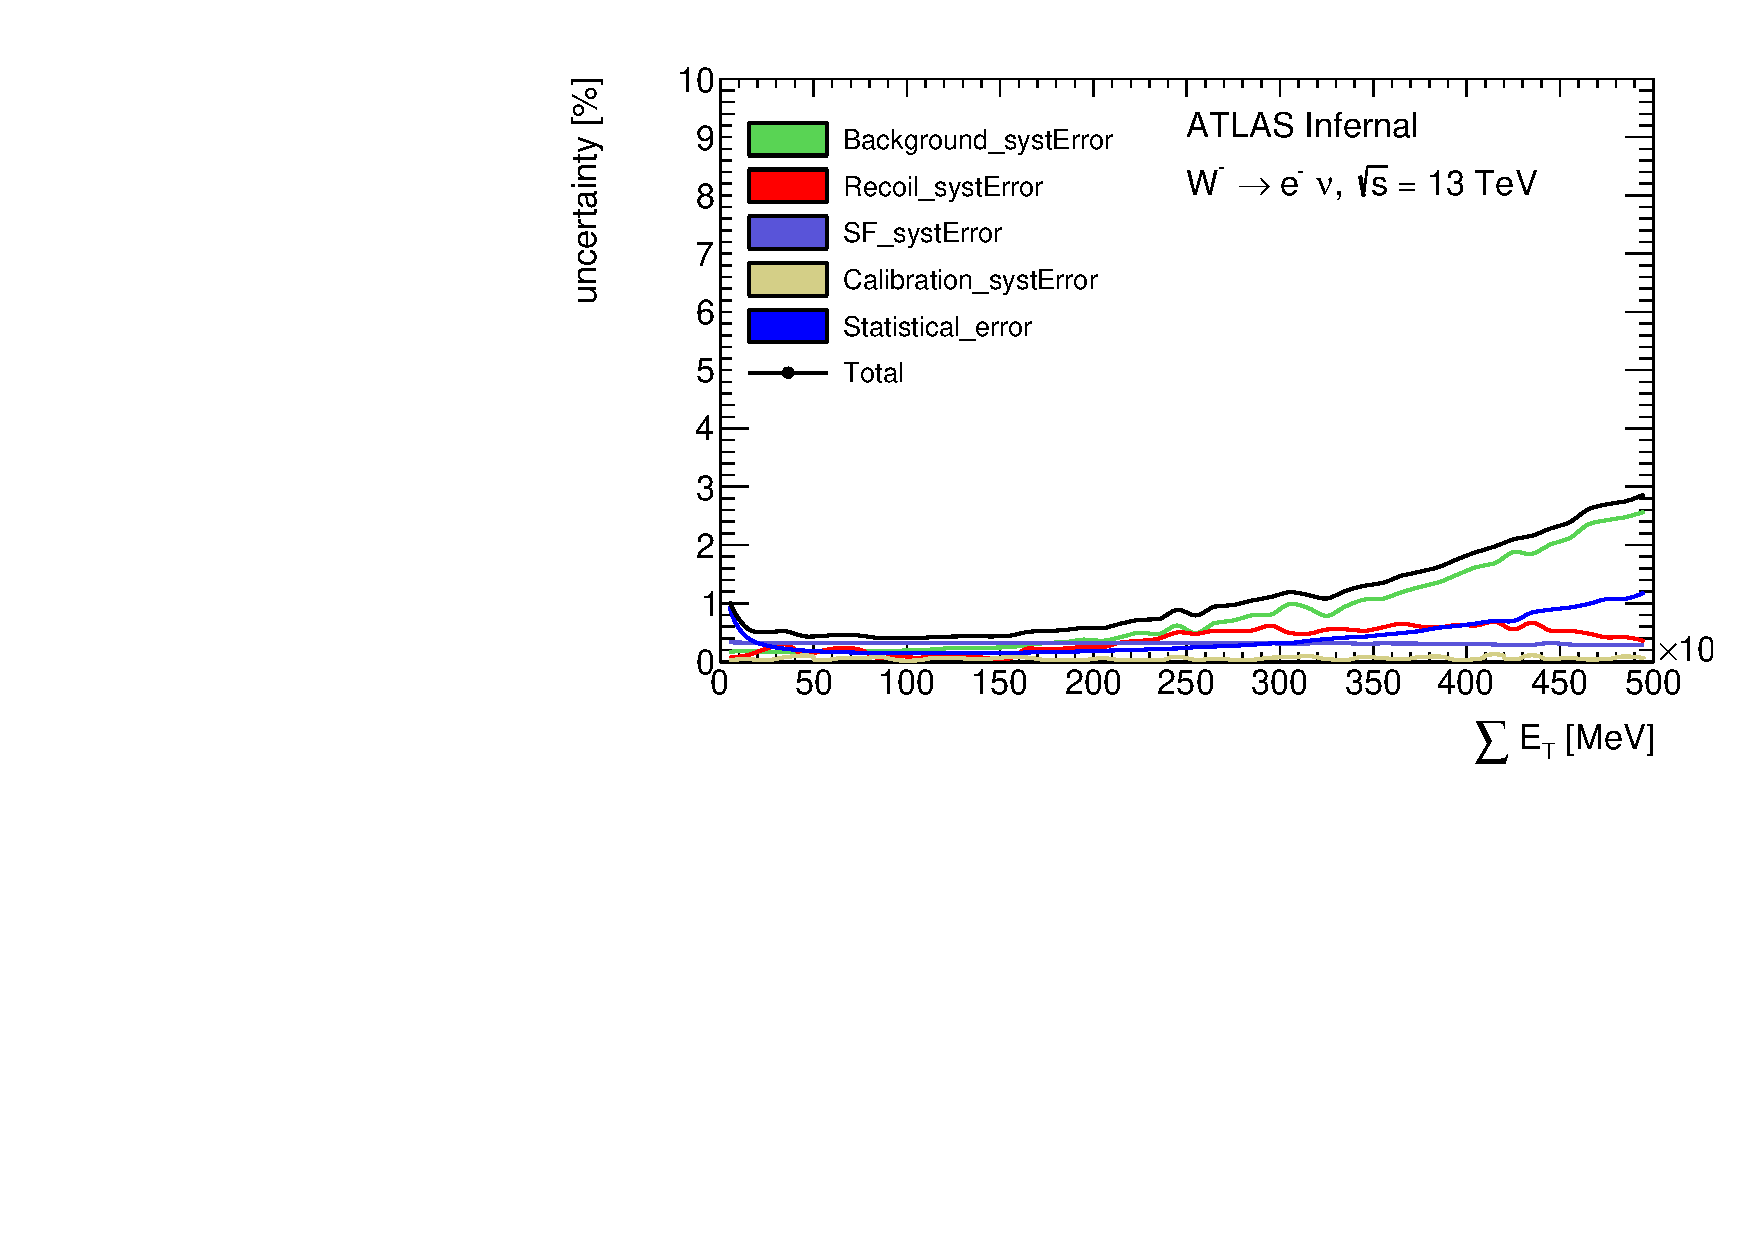
\includegraphics[width=.49\textwidth]{errors_SET_cut7_minusenu_13TeV__NormErr.pdf}\label{f:}}
	{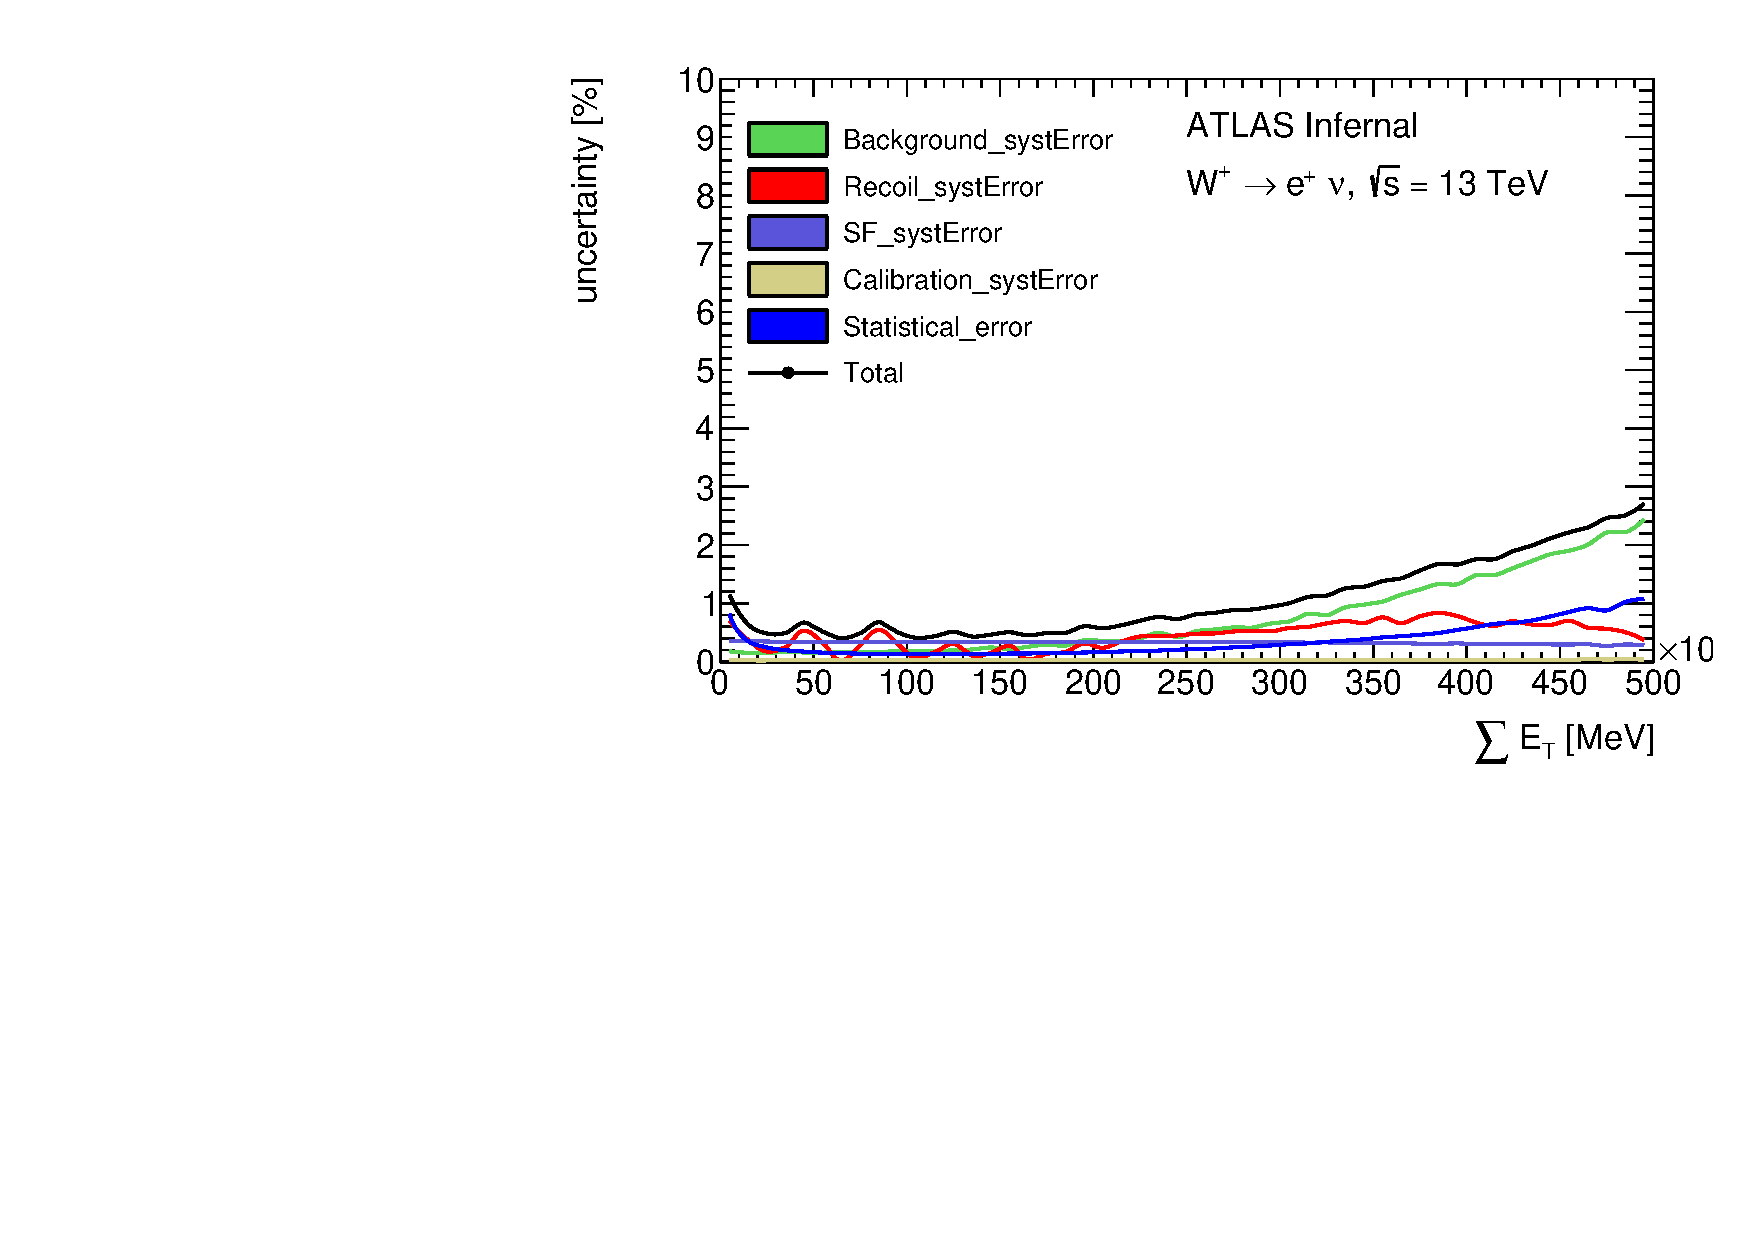
\includegraphics[width=.49\textwidth]{errors_SET_cut7_plusenu_13TeV__NormErr.pdf}\label{f:}}
		
	\caption{$\Sigma{E_T}$ systematic error breakdown in the muon and electron channel  for the $\sqrt{s} = 5$~\TeV\ and $\sqrt{s} = 13$~\TeV\ datasets.}
\end{figure}
\newpage


\begin{figure}[h]
	\centering
	{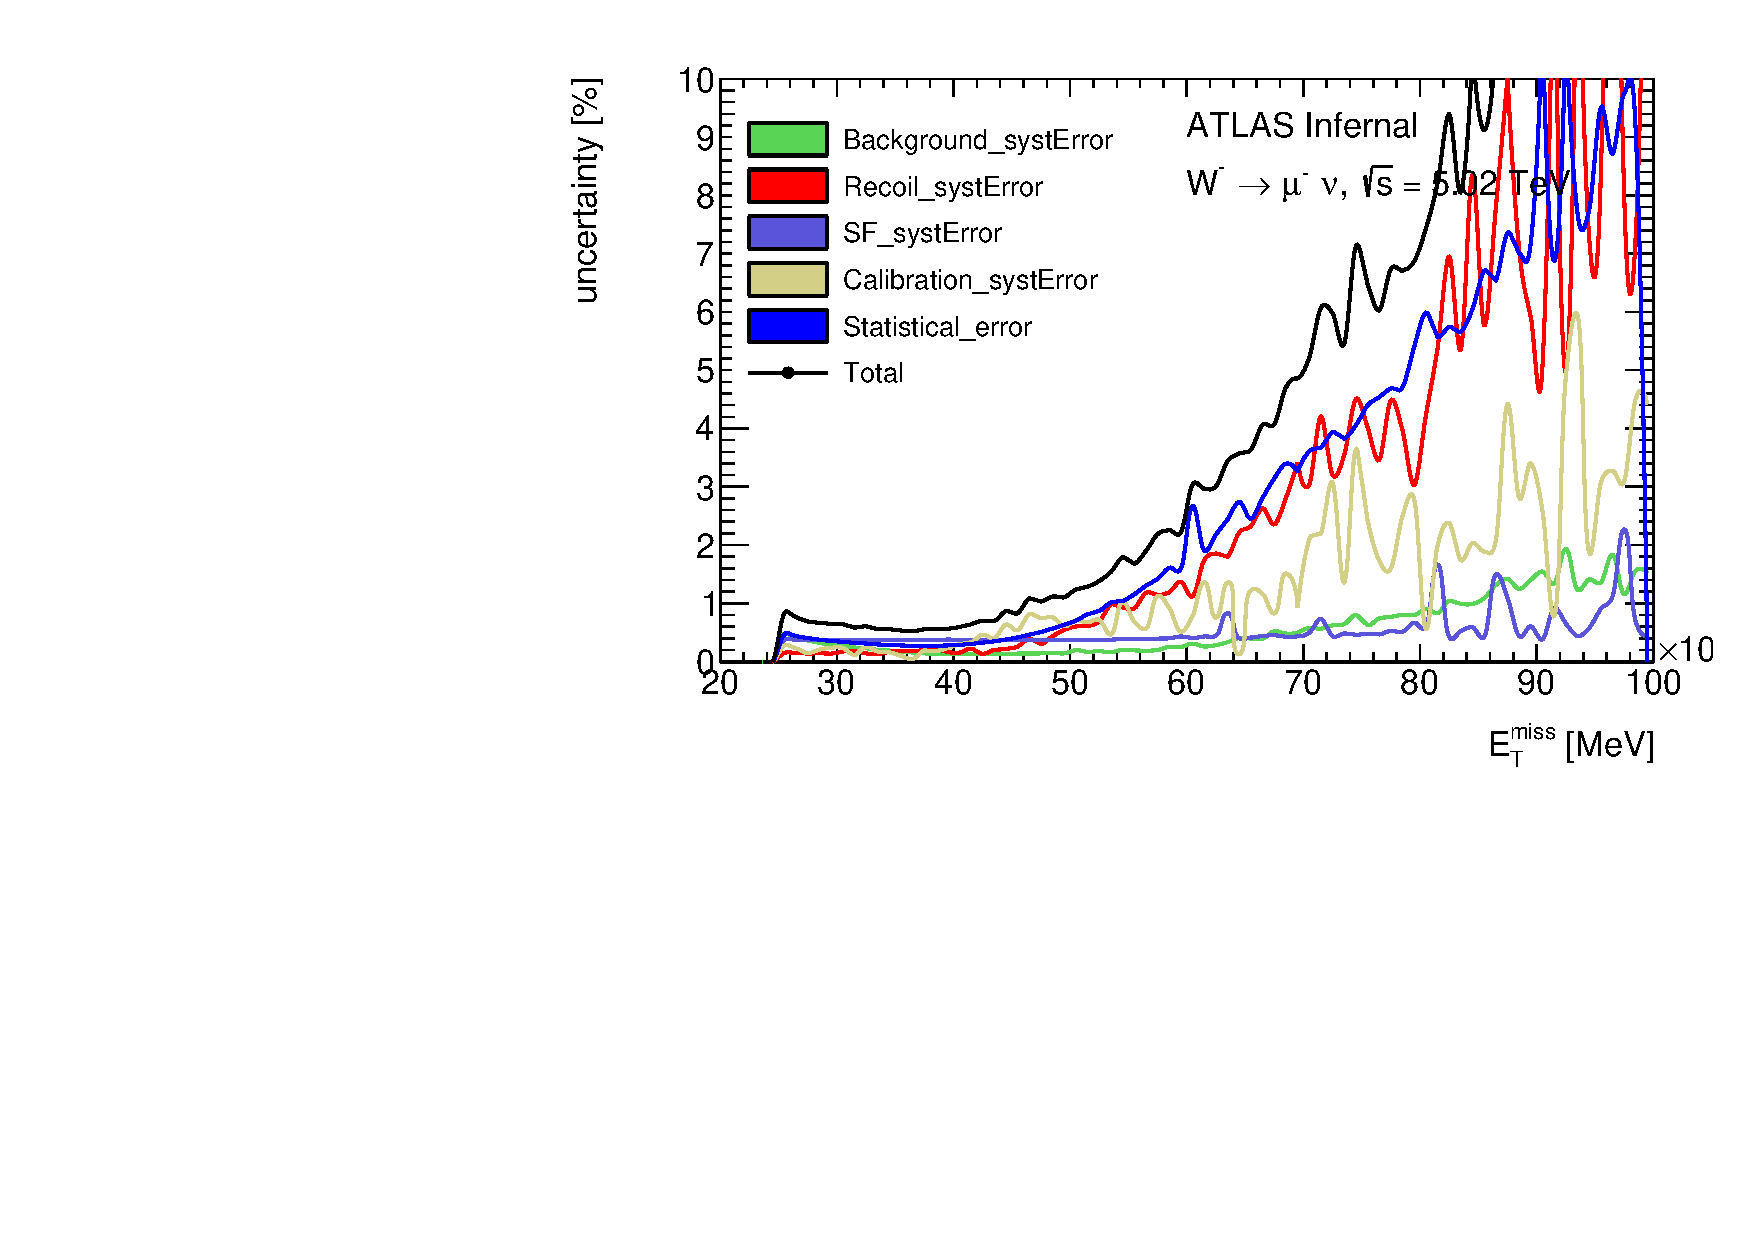
\includegraphics[width=.49\textwidth]{errors_met_cut7_minusmunu_5TeV__NormErr.pdf}\label{f:}}
	{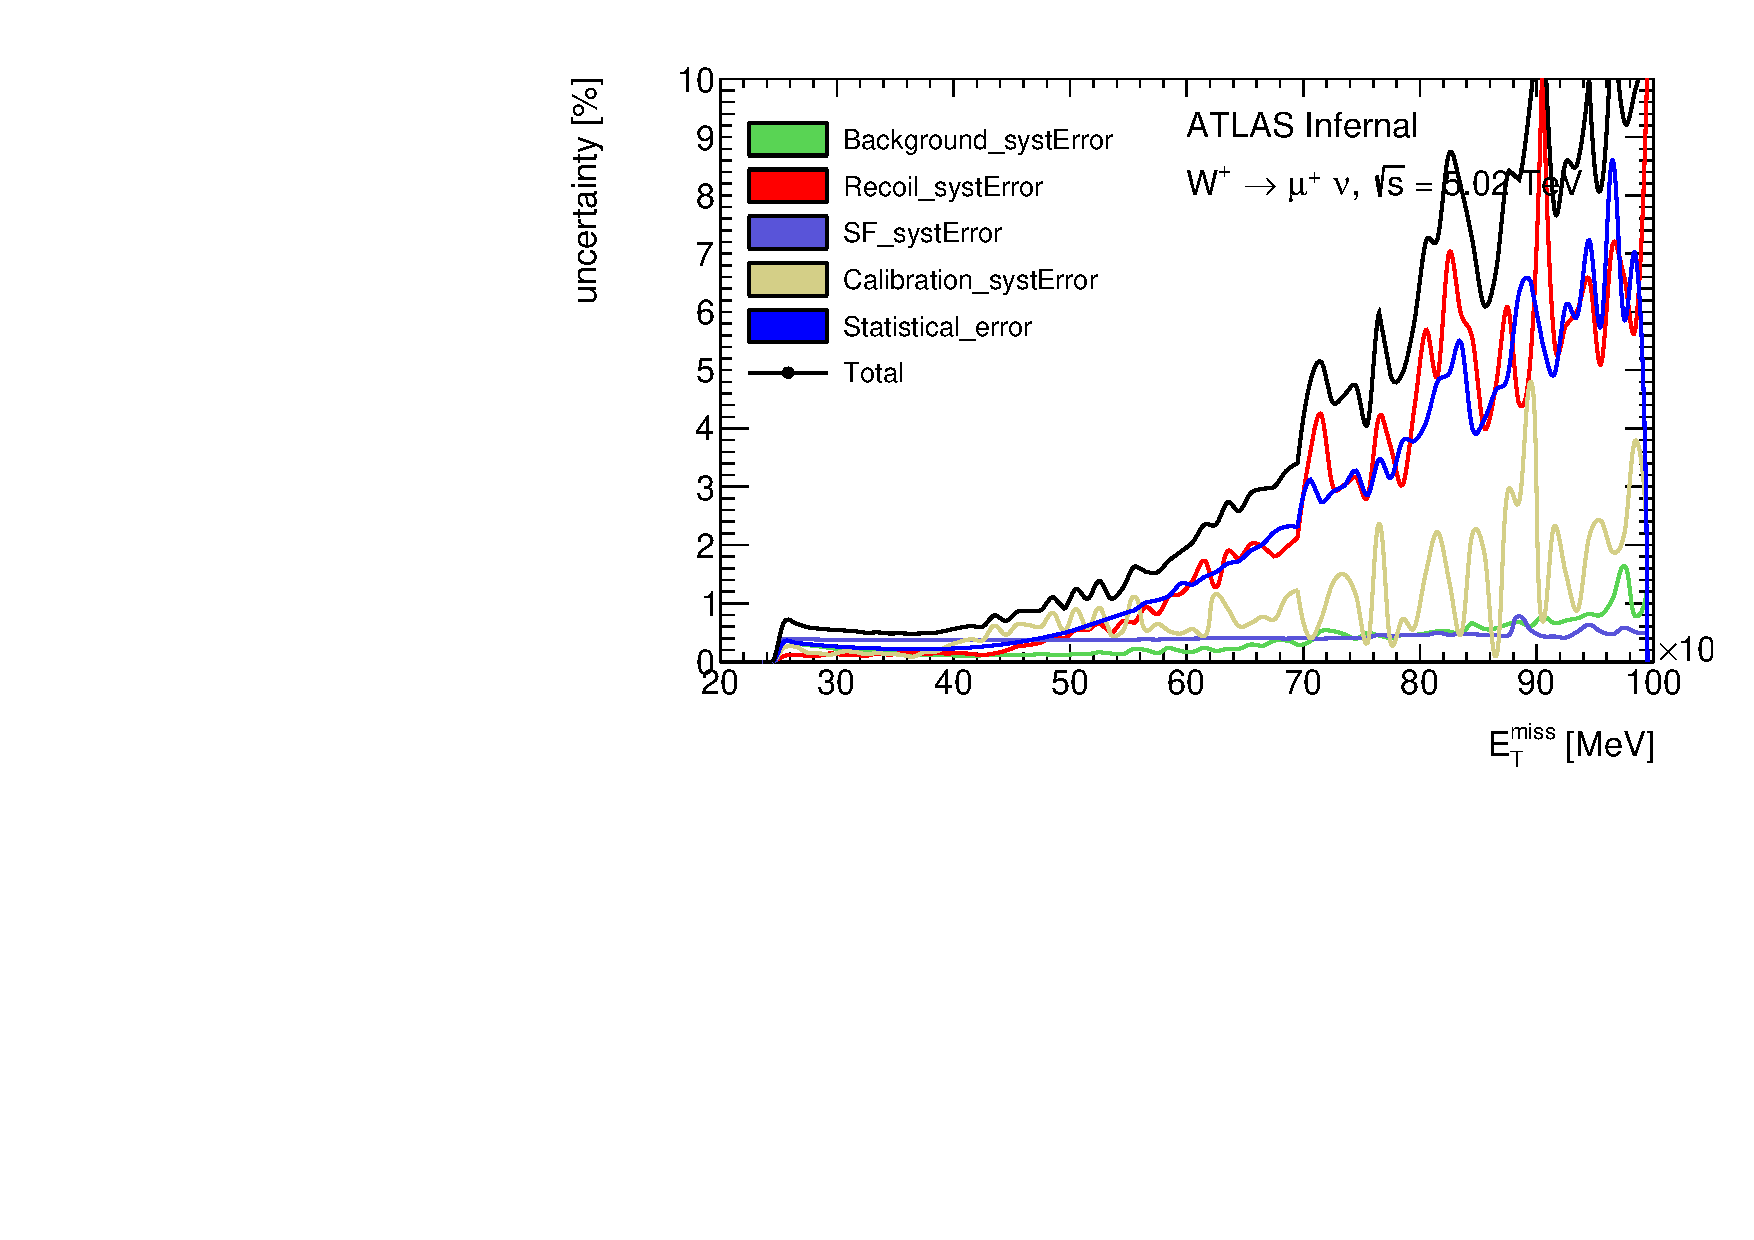
\includegraphics[width=.49\textwidth]{errors_met_cut7_plusmunu_5TeV__NormErr.pdf}\label{f:}}
	
	{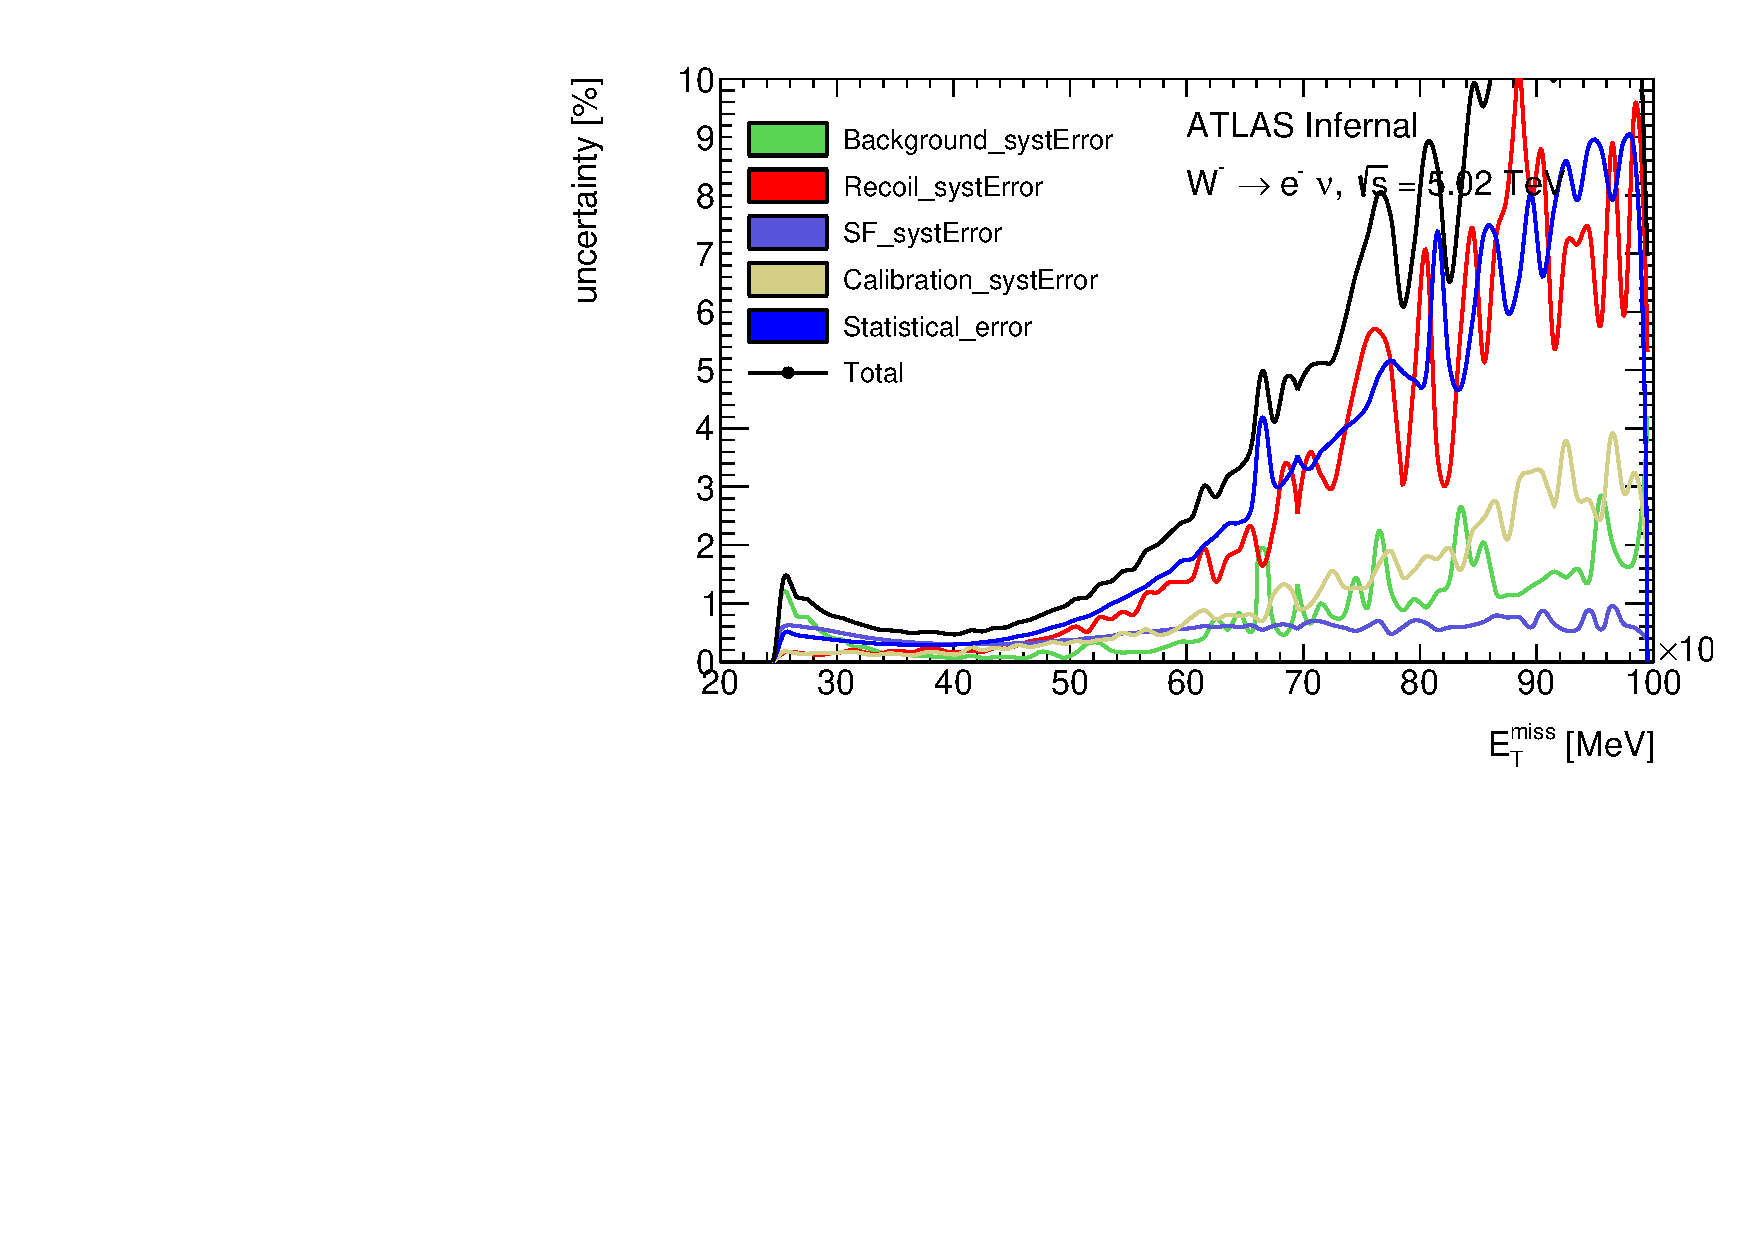
\includegraphics[width=.49\textwidth]{errors_met_cut7_minusenu_5TeV__NormErr.pdf}\label{f:}}
	{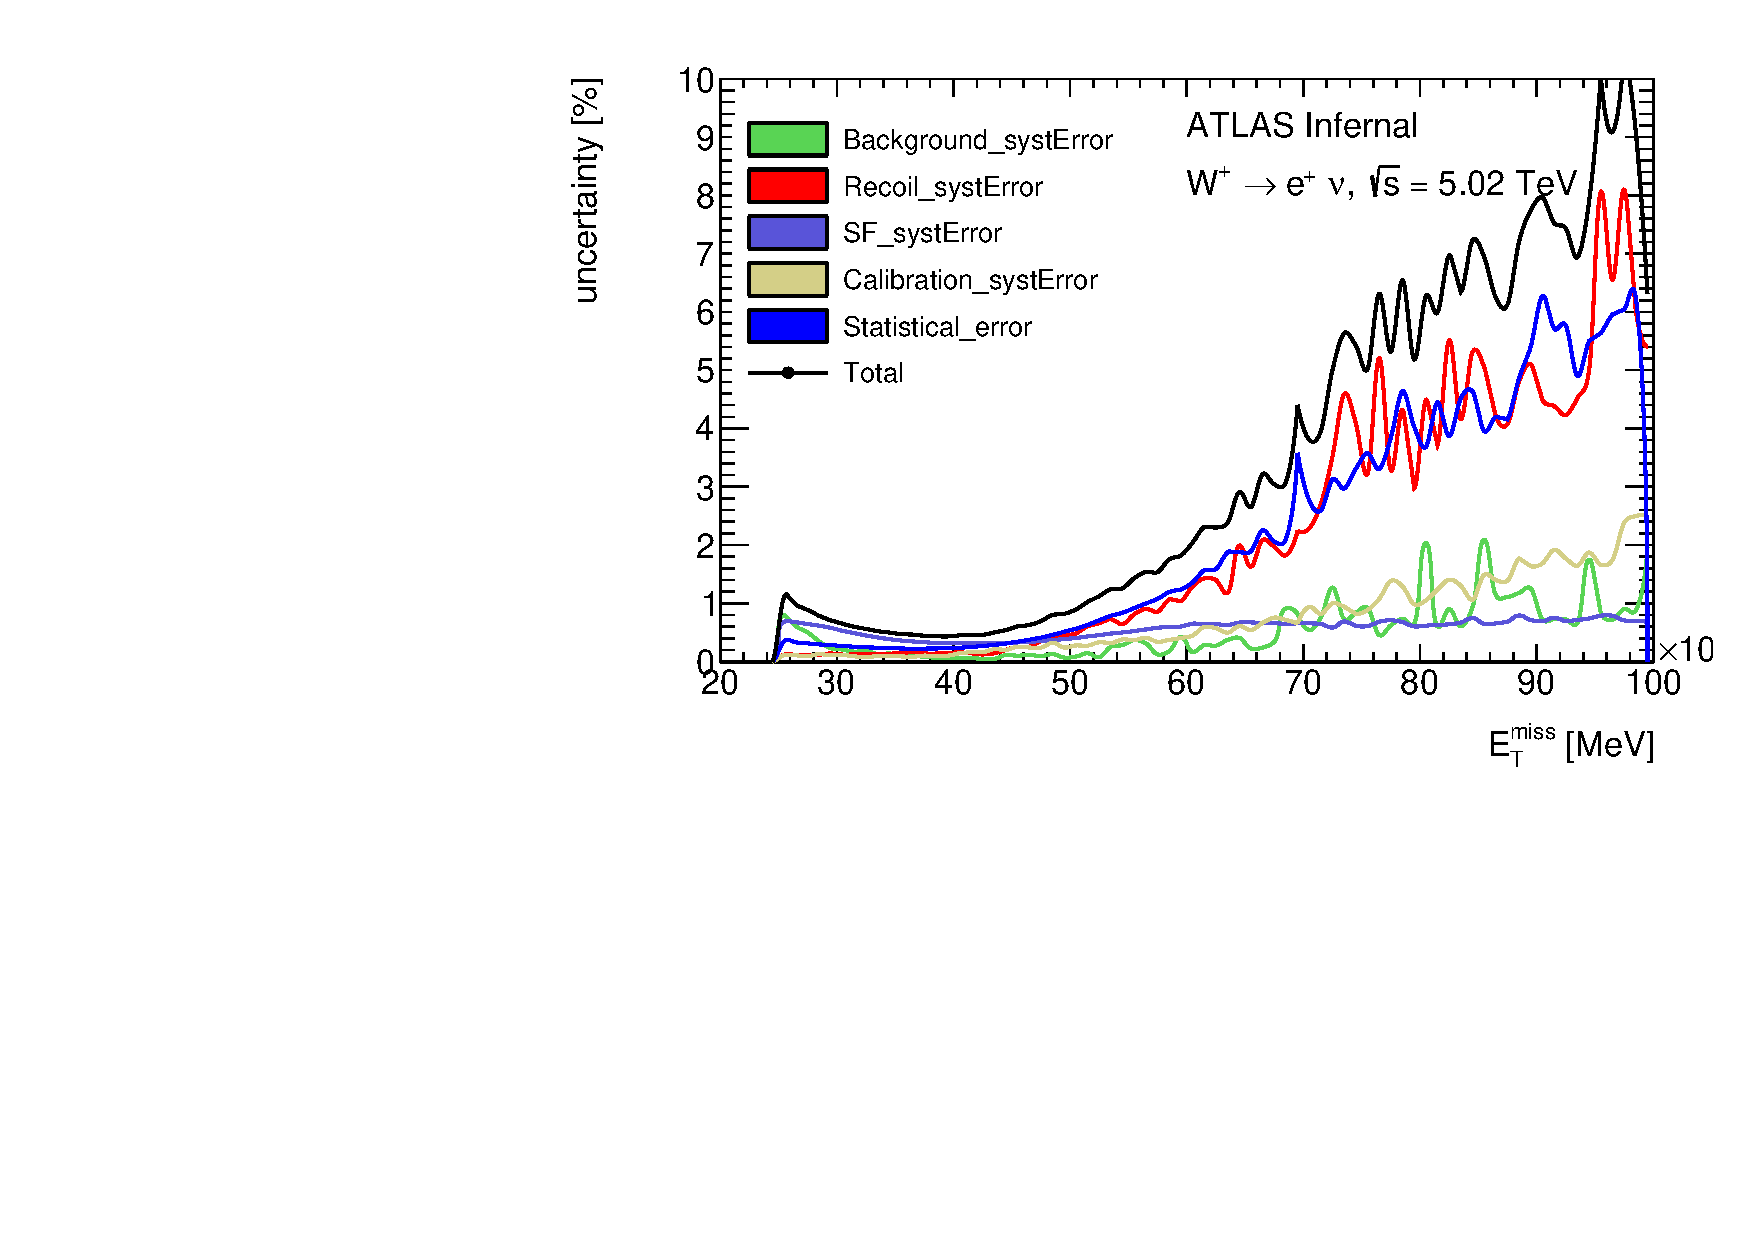
\includegraphics[width=.49\textwidth]{errors_met_cut7_plusenu_5TeV__NormErr.pdf}\label{f:}}
	
		{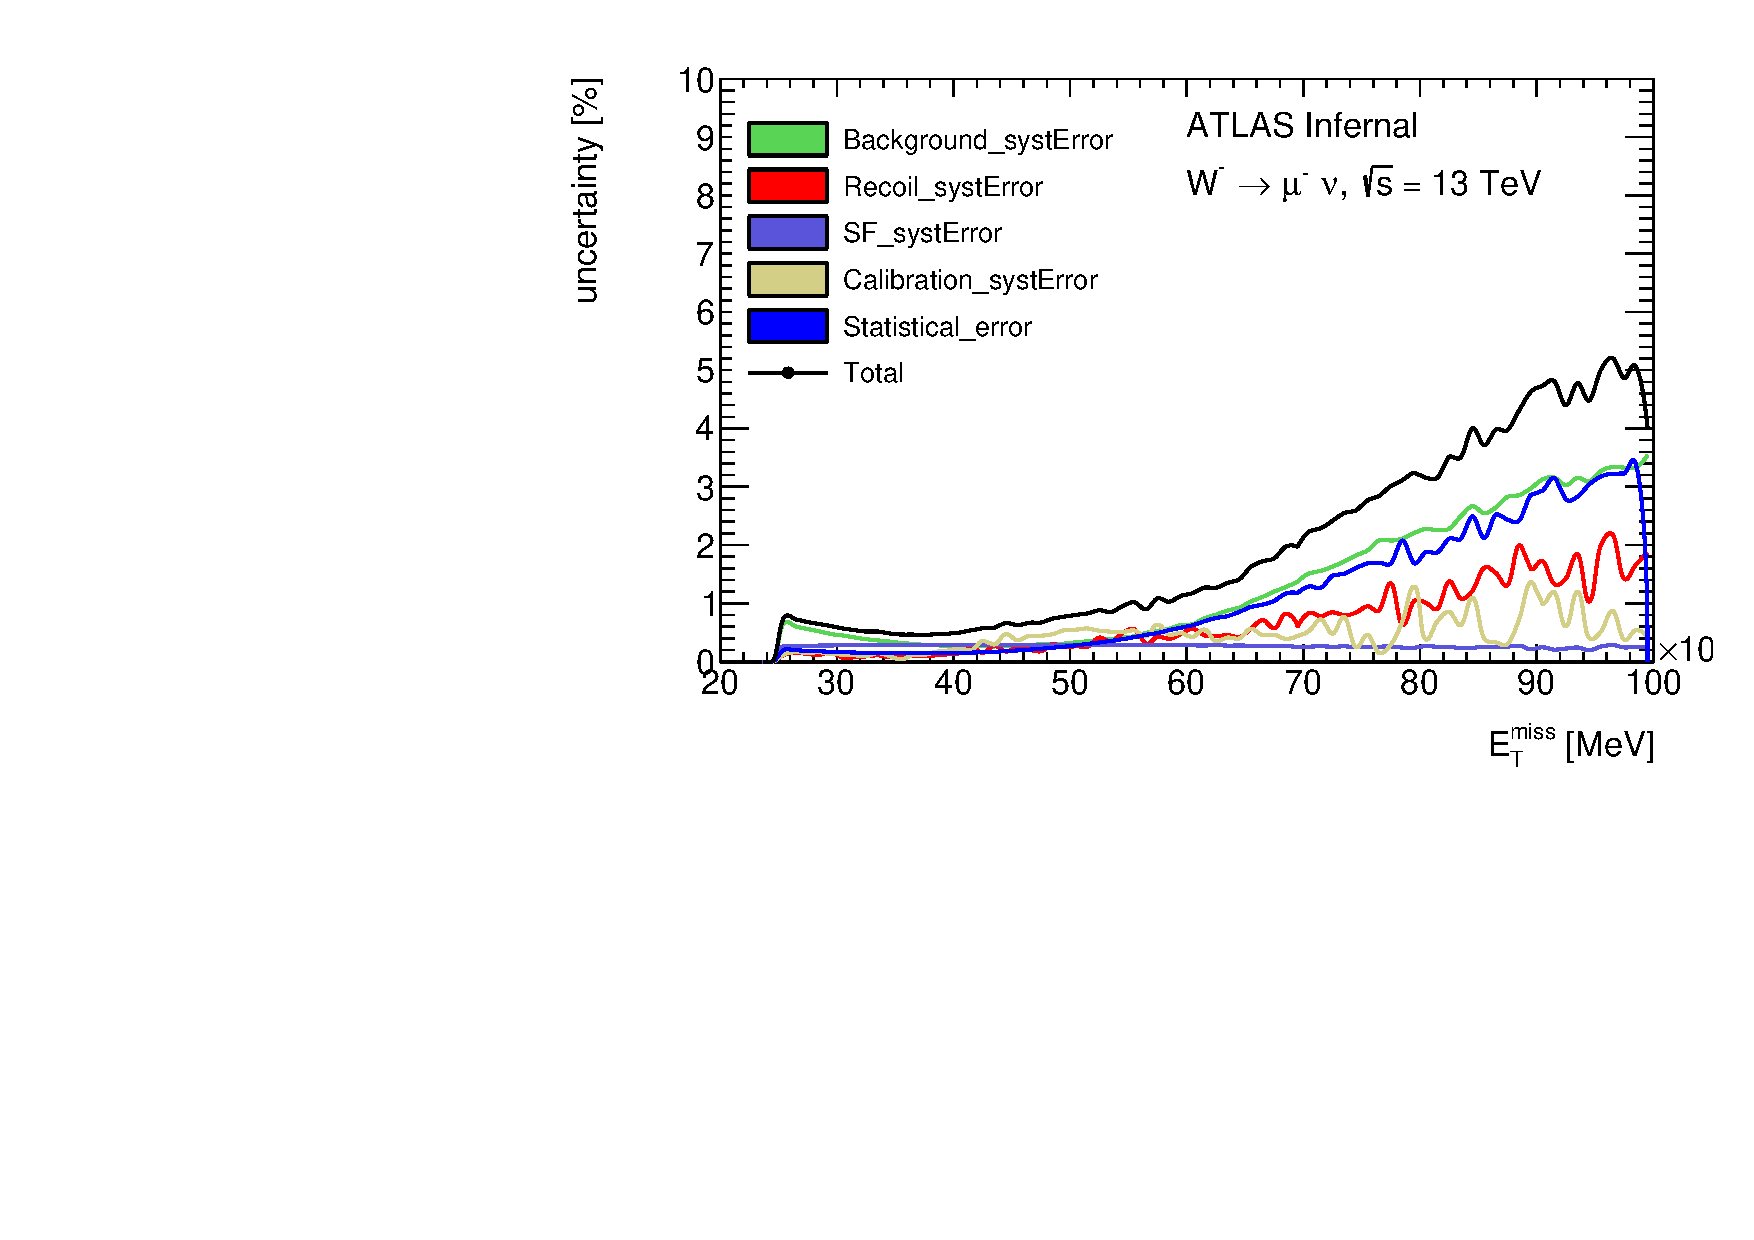
\includegraphics[width=.49\textwidth]{errors_met_cut7_minusmunu_13TeV__NormErr.pdf}\label{f:}}
	{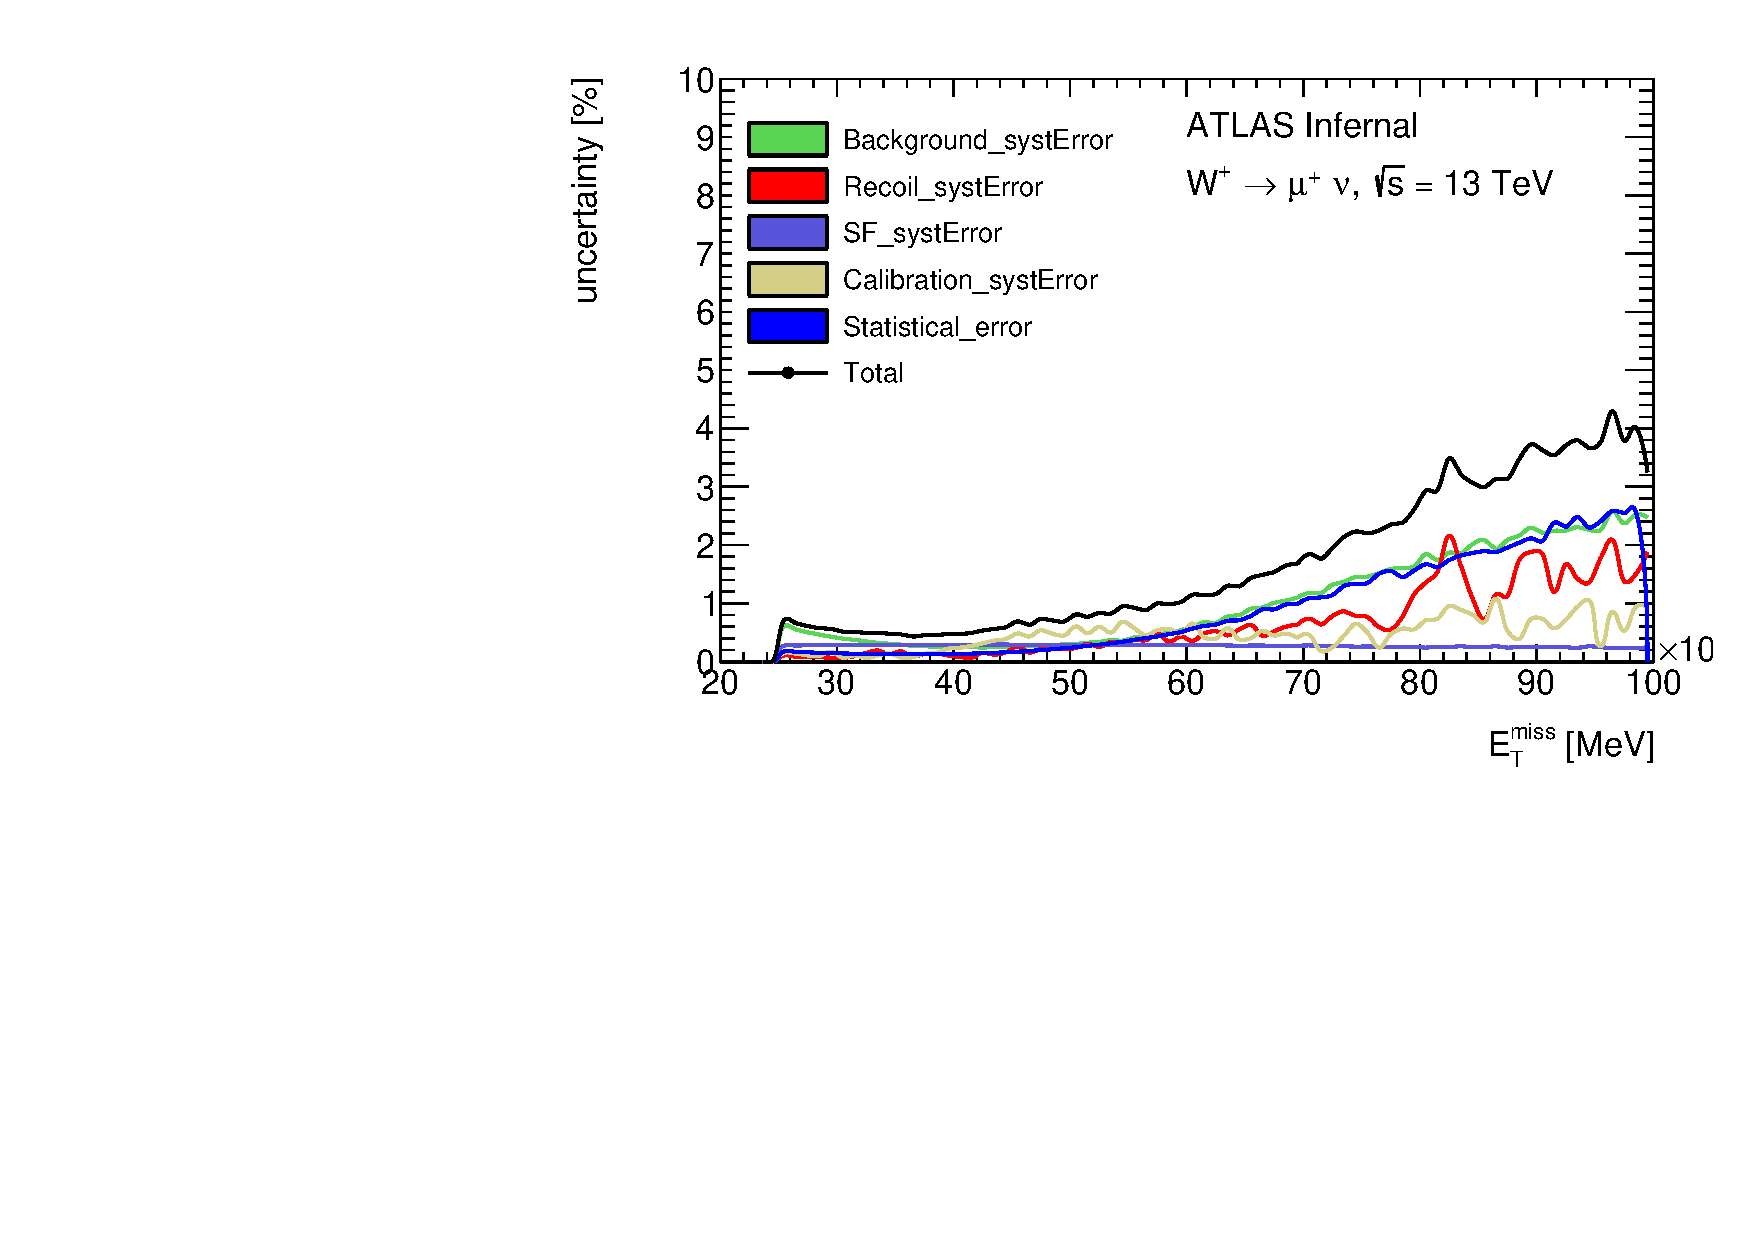
\includegraphics[width=.49\textwidth]{errors_met_cut7_plusmunu_13TeV__NormErr.pdf}\label{f:}}
	
	{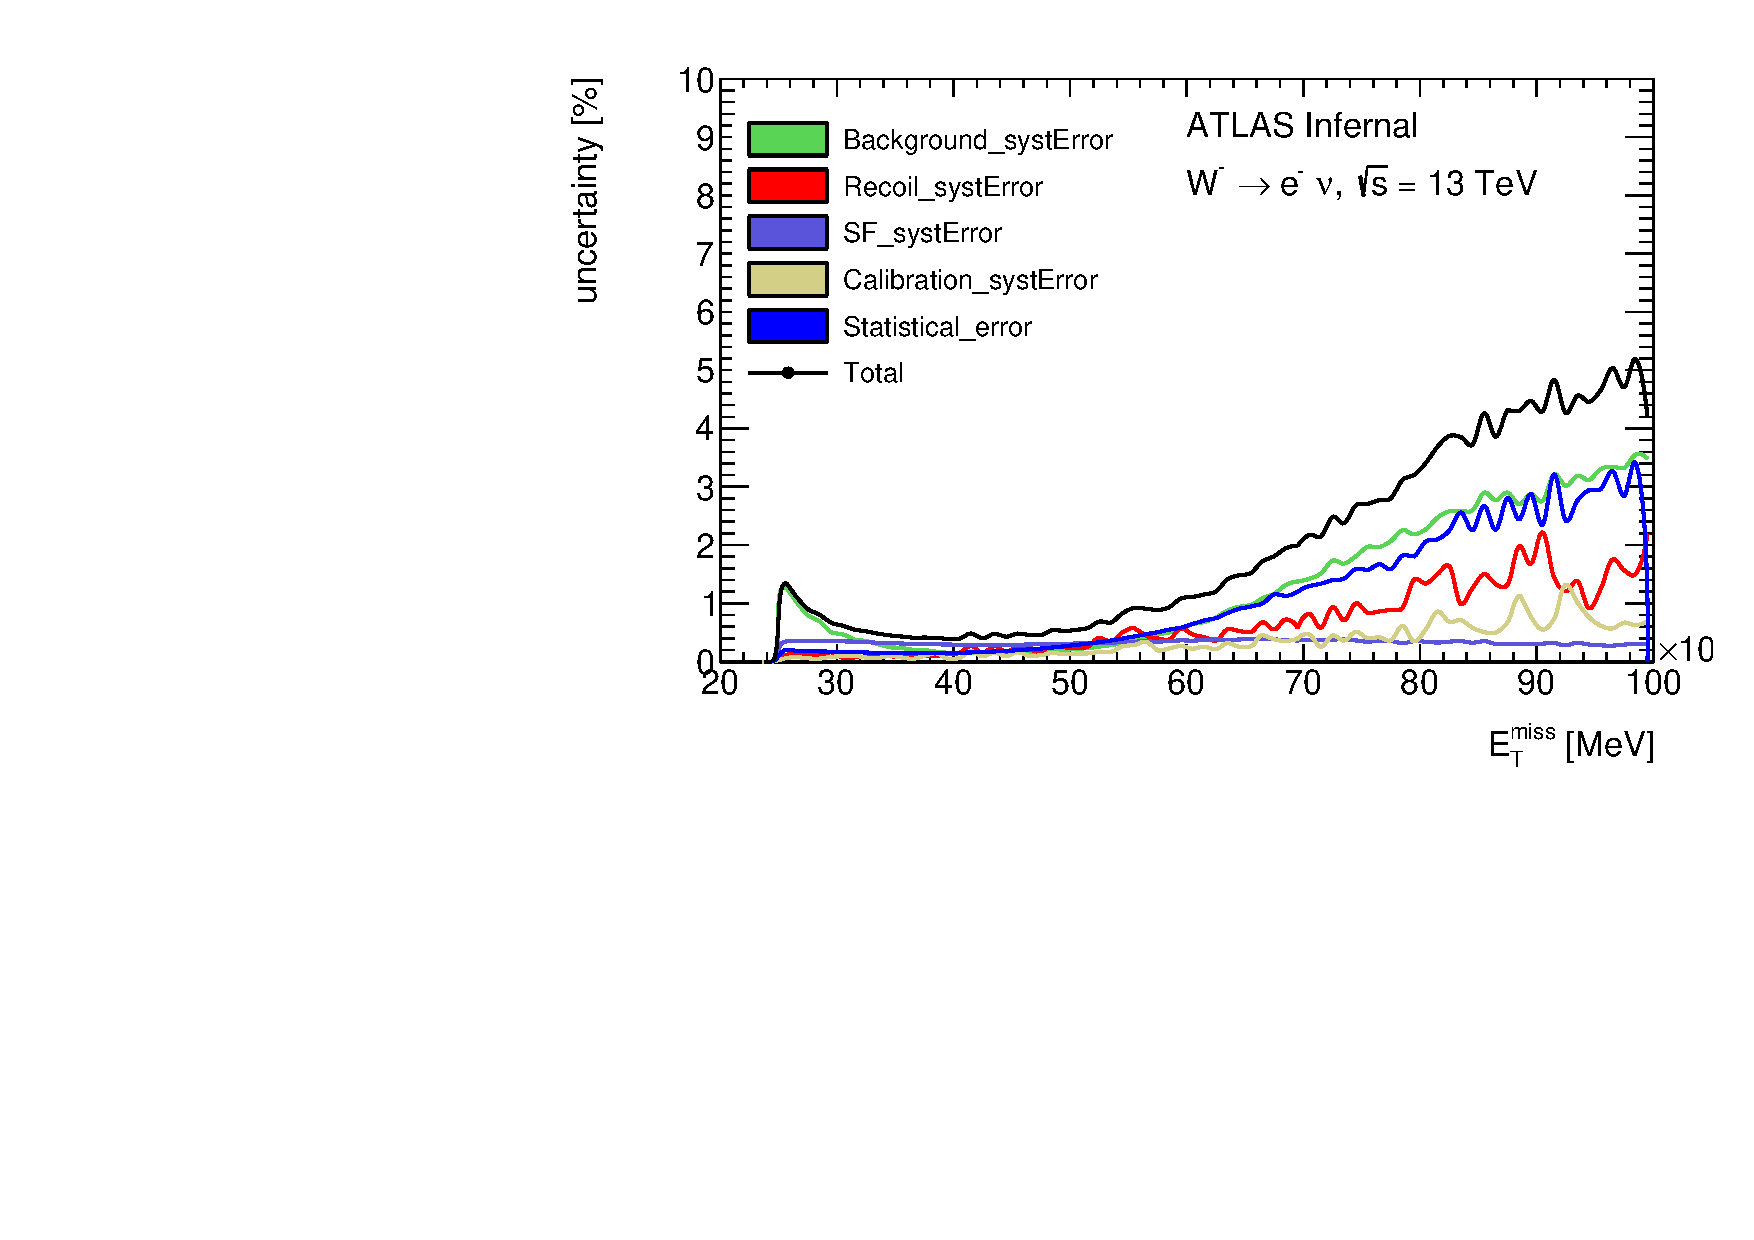
\includegraphics[width=.49\textwidth]{errors_met_cut7_minusenu_13TeV__NormErr.pdf}\label{f:}}
	{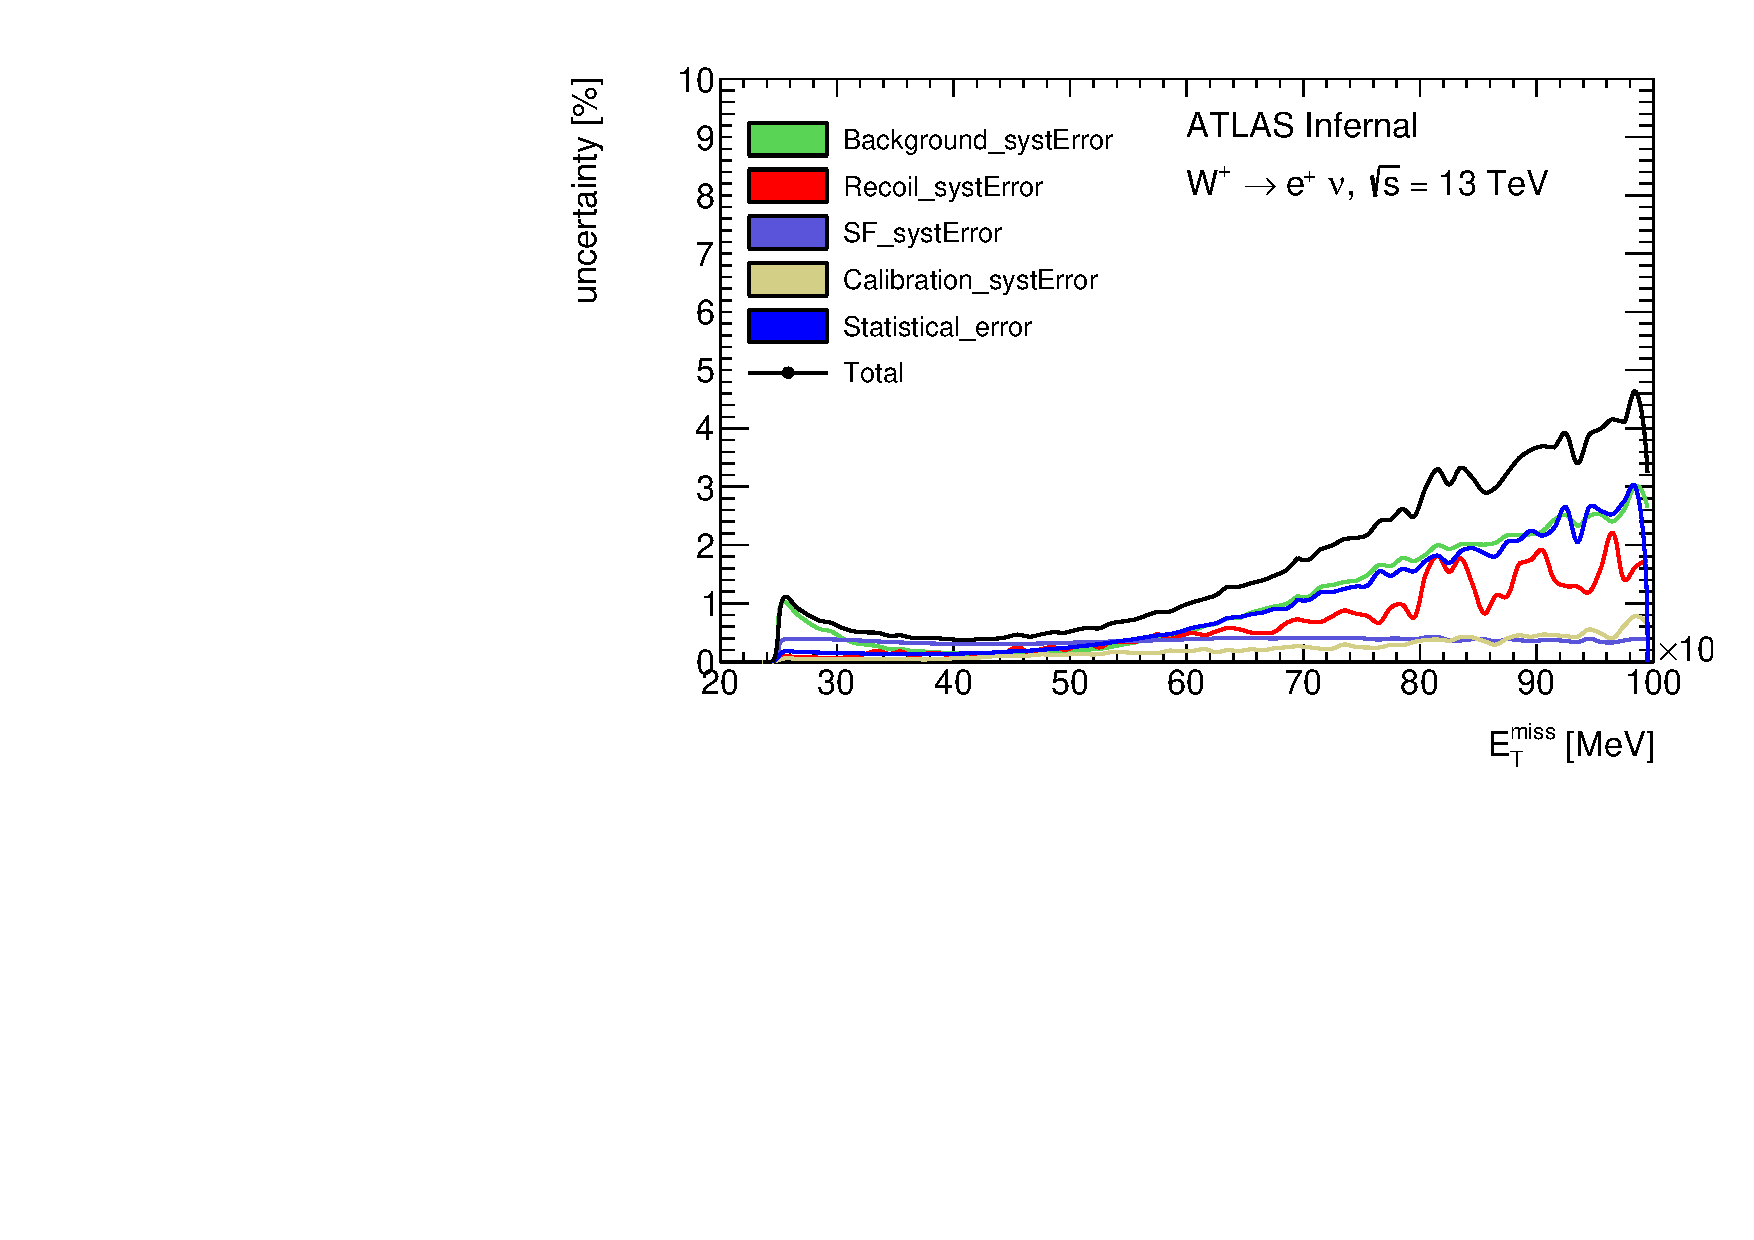
\includegraphics[width=.49\textwidth]{errors_met_cut7_plusenu_13TeV__NormErr.pdf}\label{f:}}
	\caption{ $\vec{E}^{miss}_{T}$ systematic error breakdown in the muon and electron channel  for the $\sqrt{s} = 5$~\TeV\ and $\sqrt{s} = 13$~\TeV\ datasets.}
\end{figure}
\newpage



\begin{figure}[h]
	\centering
	{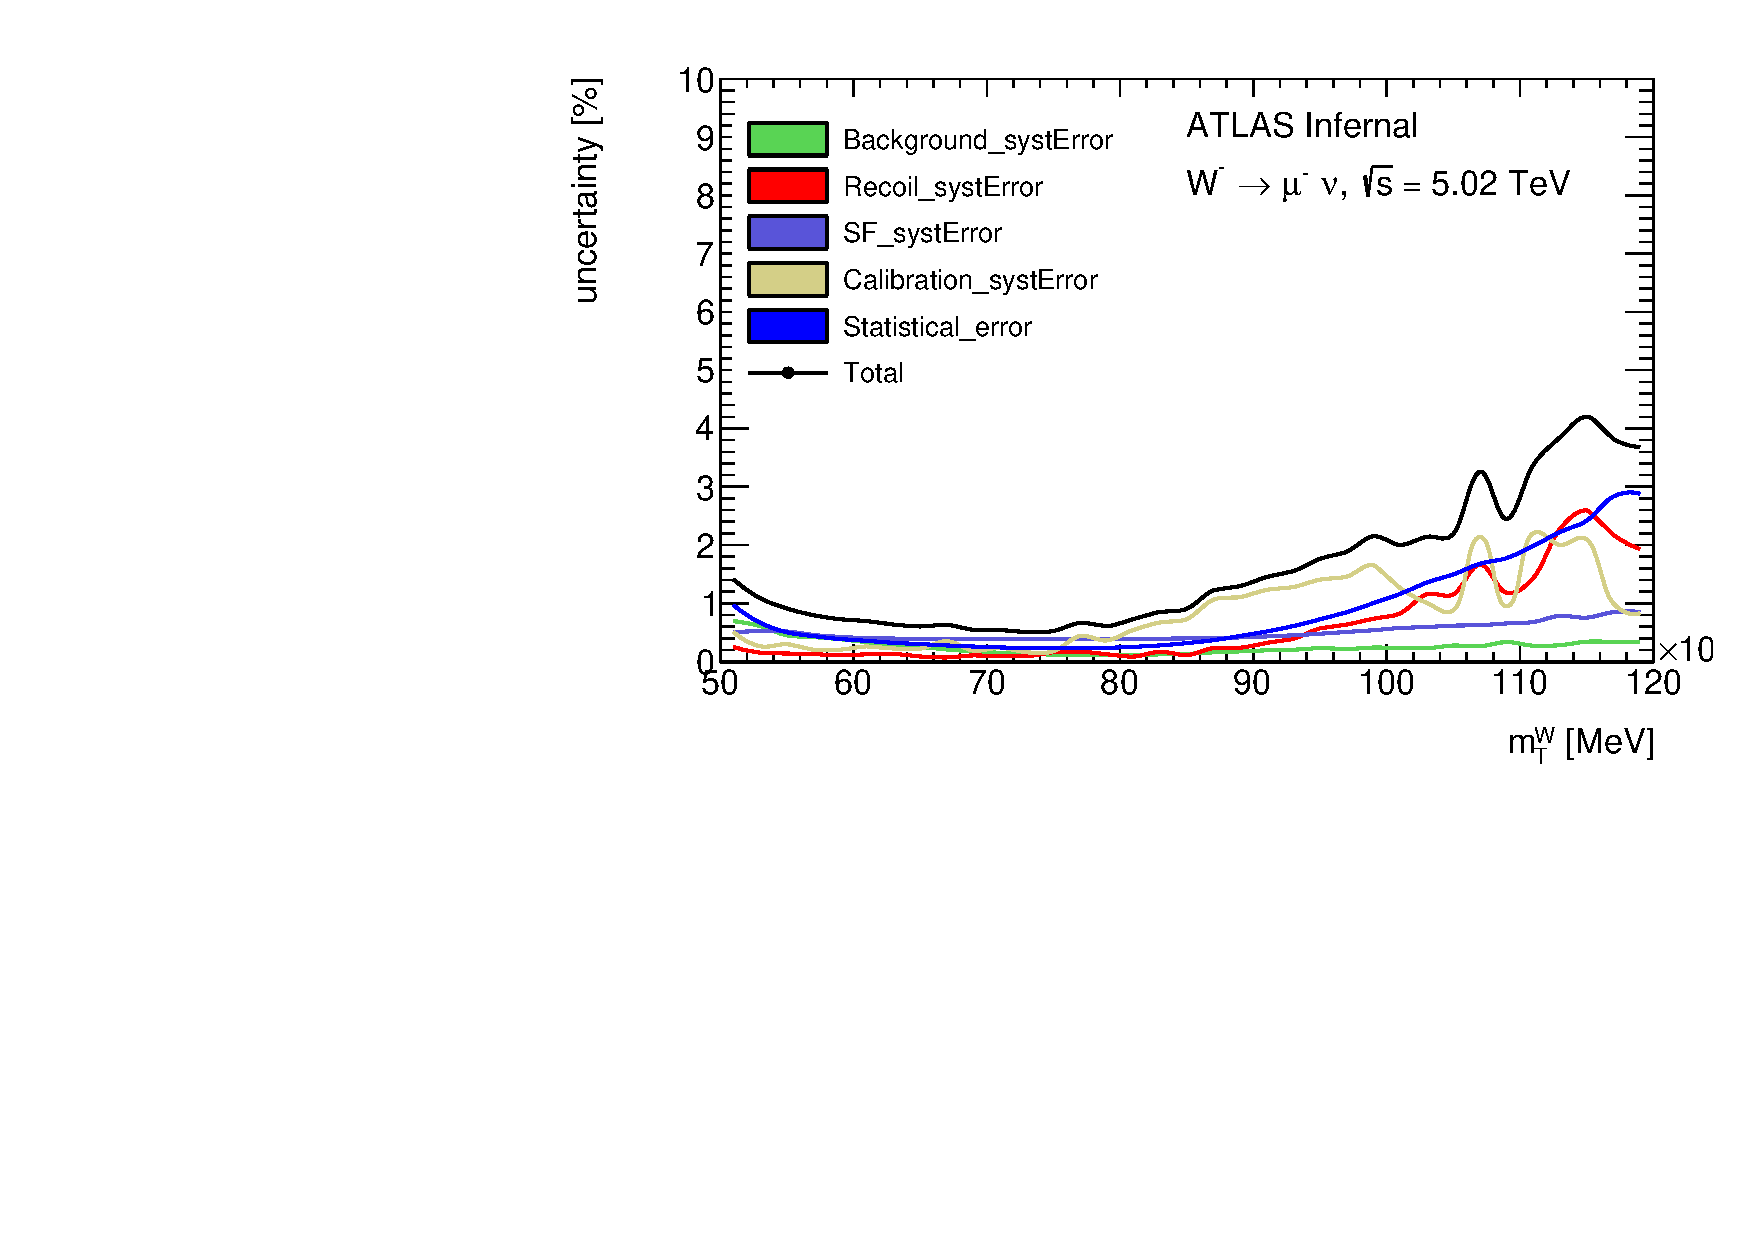
\includegraphics[width=.49\textwidth]{errors_mT_cut7_minusmunu_5TeV__NormErr.pdf}\label{f:}}
	{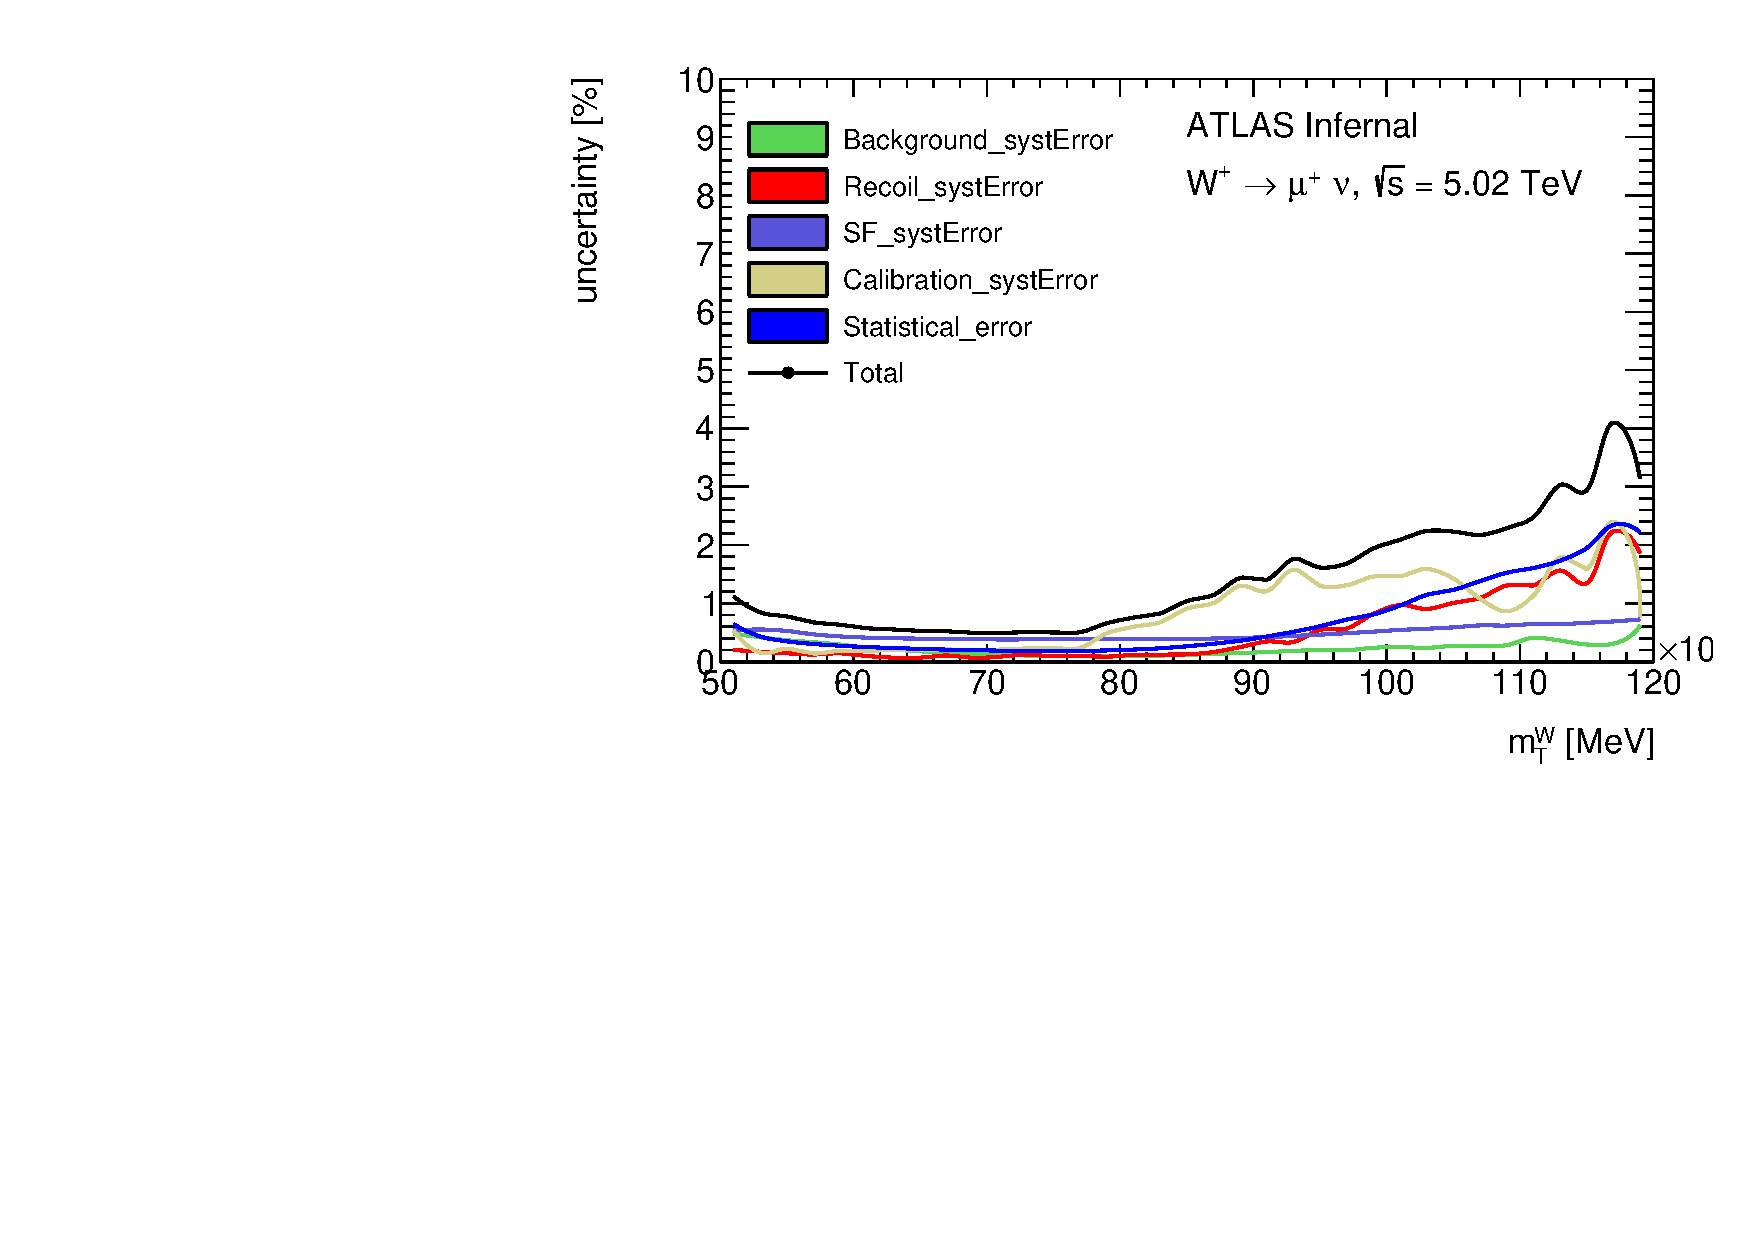
\includegraphics[width=.49\textwidth]{errors_mT_cut7_plusmunu_5TeV__NormErr.pdf}\label{f:}}
	
	{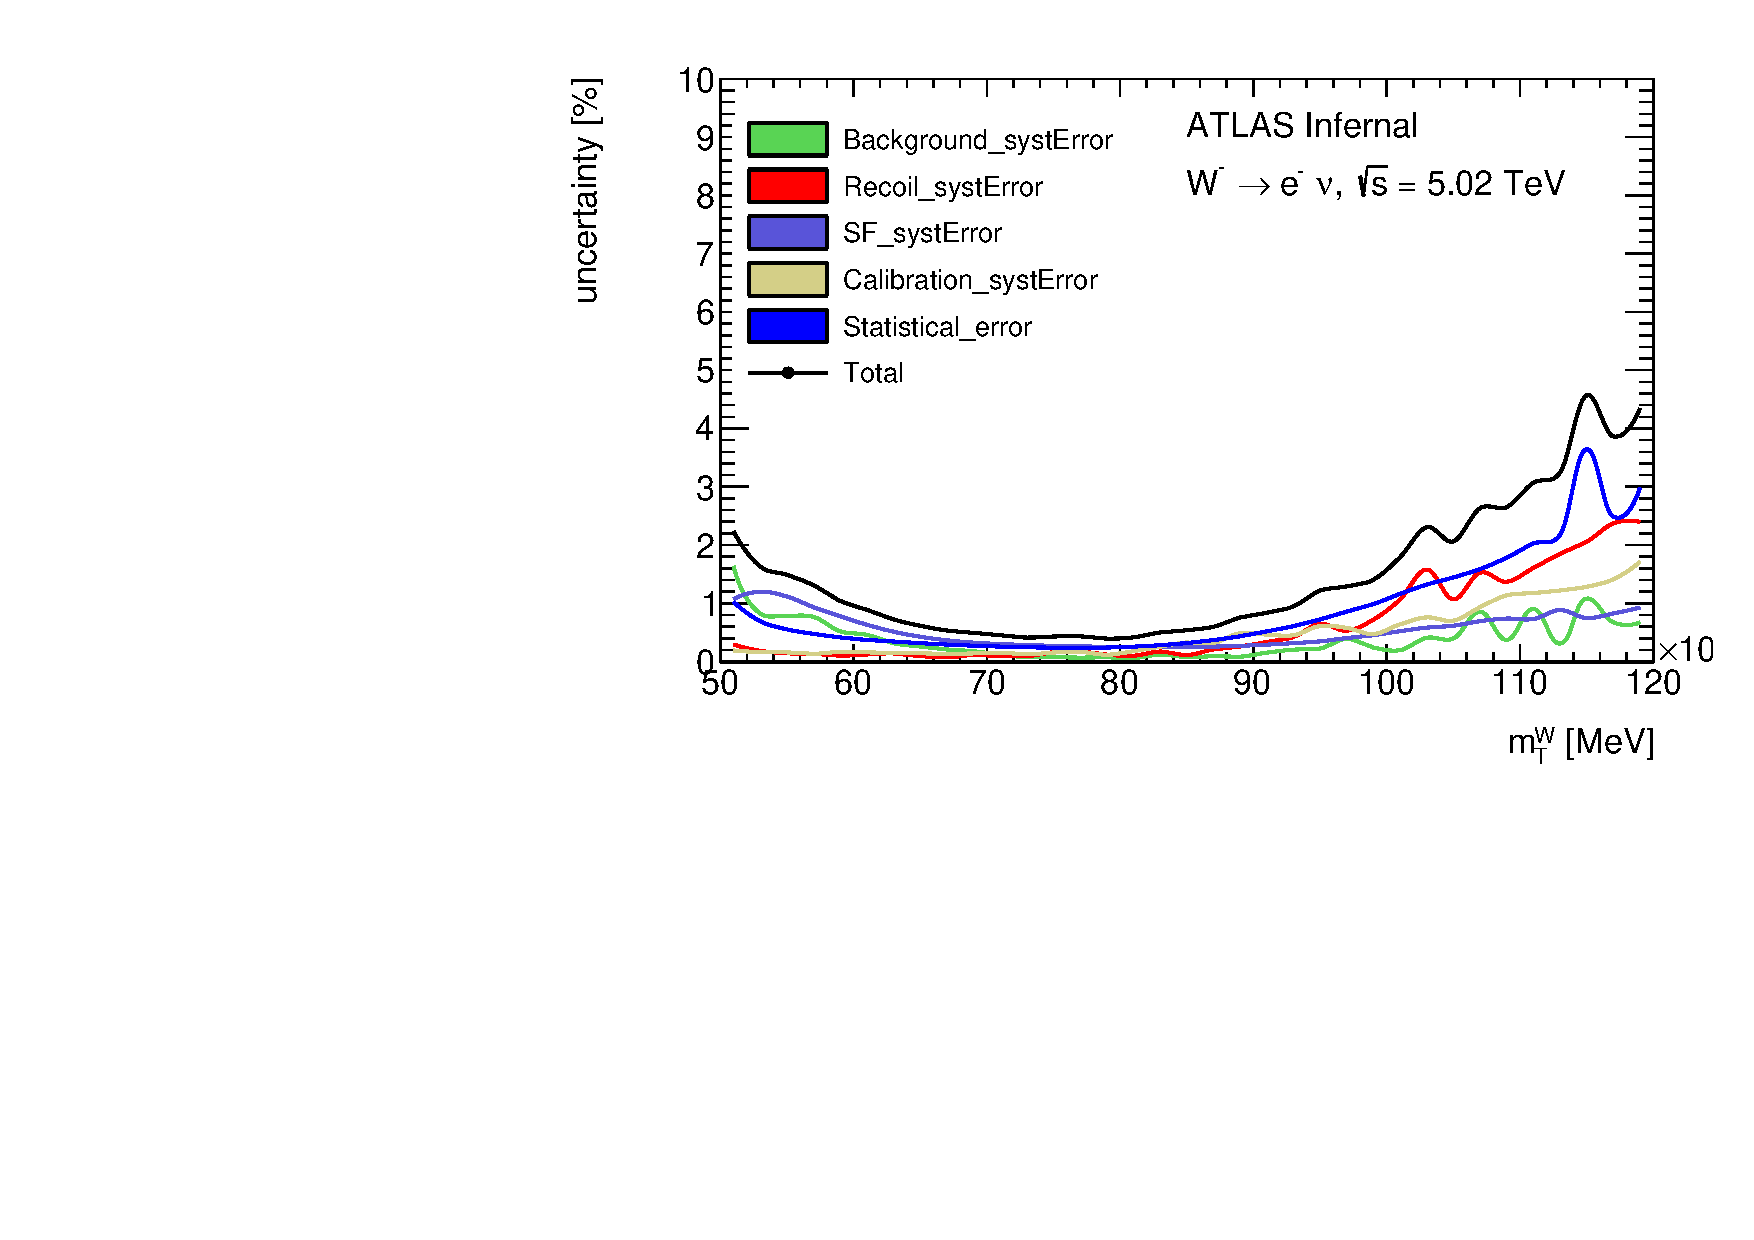
\includegraphics[width=.49\textwidth]{errors_mT_cut7_minusenu_5TeV__NormErr.pdf}\label{f:}}
	{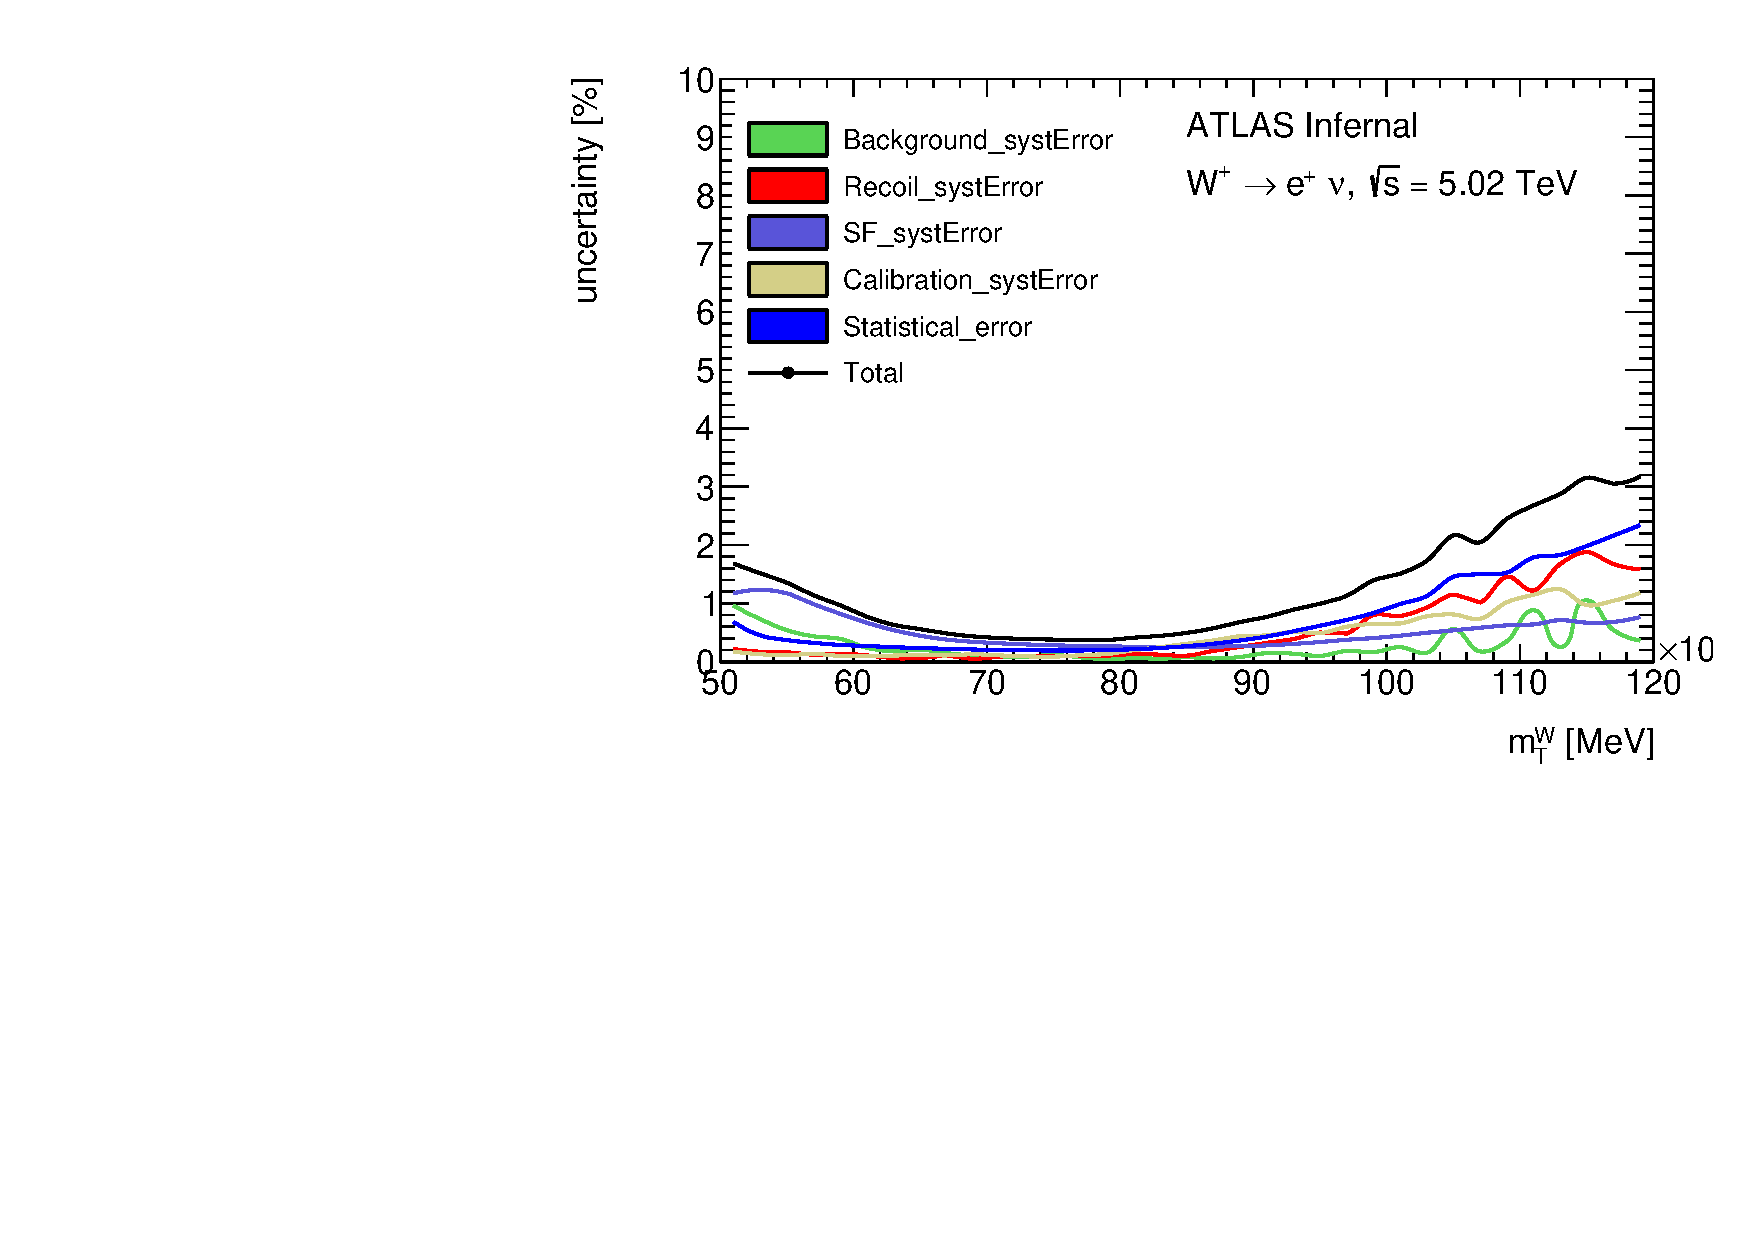
\includegraphics[width=.49\textwidth]{errors_mT_cut7_plusenu_5TeV__NormErr.pdf}\label{f:}}
	
		{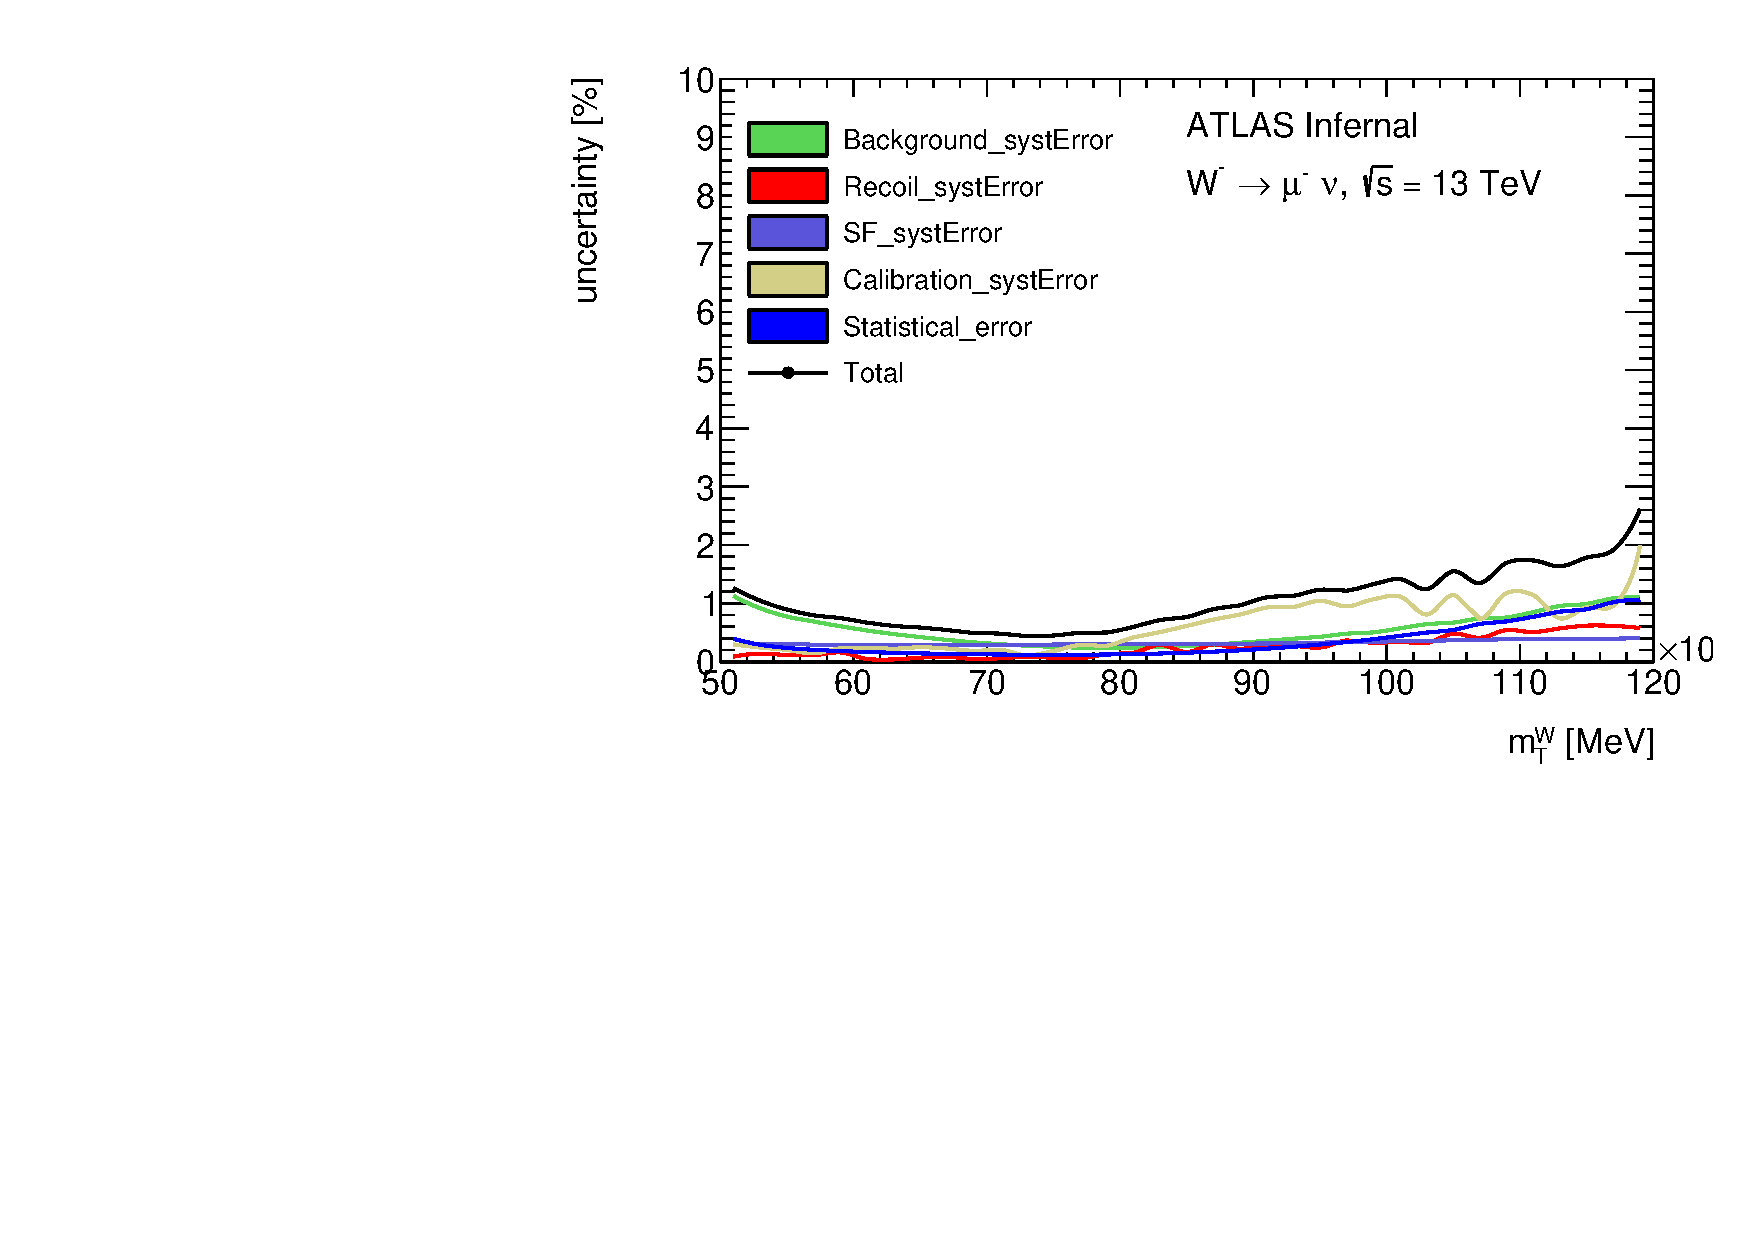
\includegraphics[width=.49\textwidth]{errors_mT_cut7_minusmunu_13TeV__NormErr.pdf}\label{f:}}
	{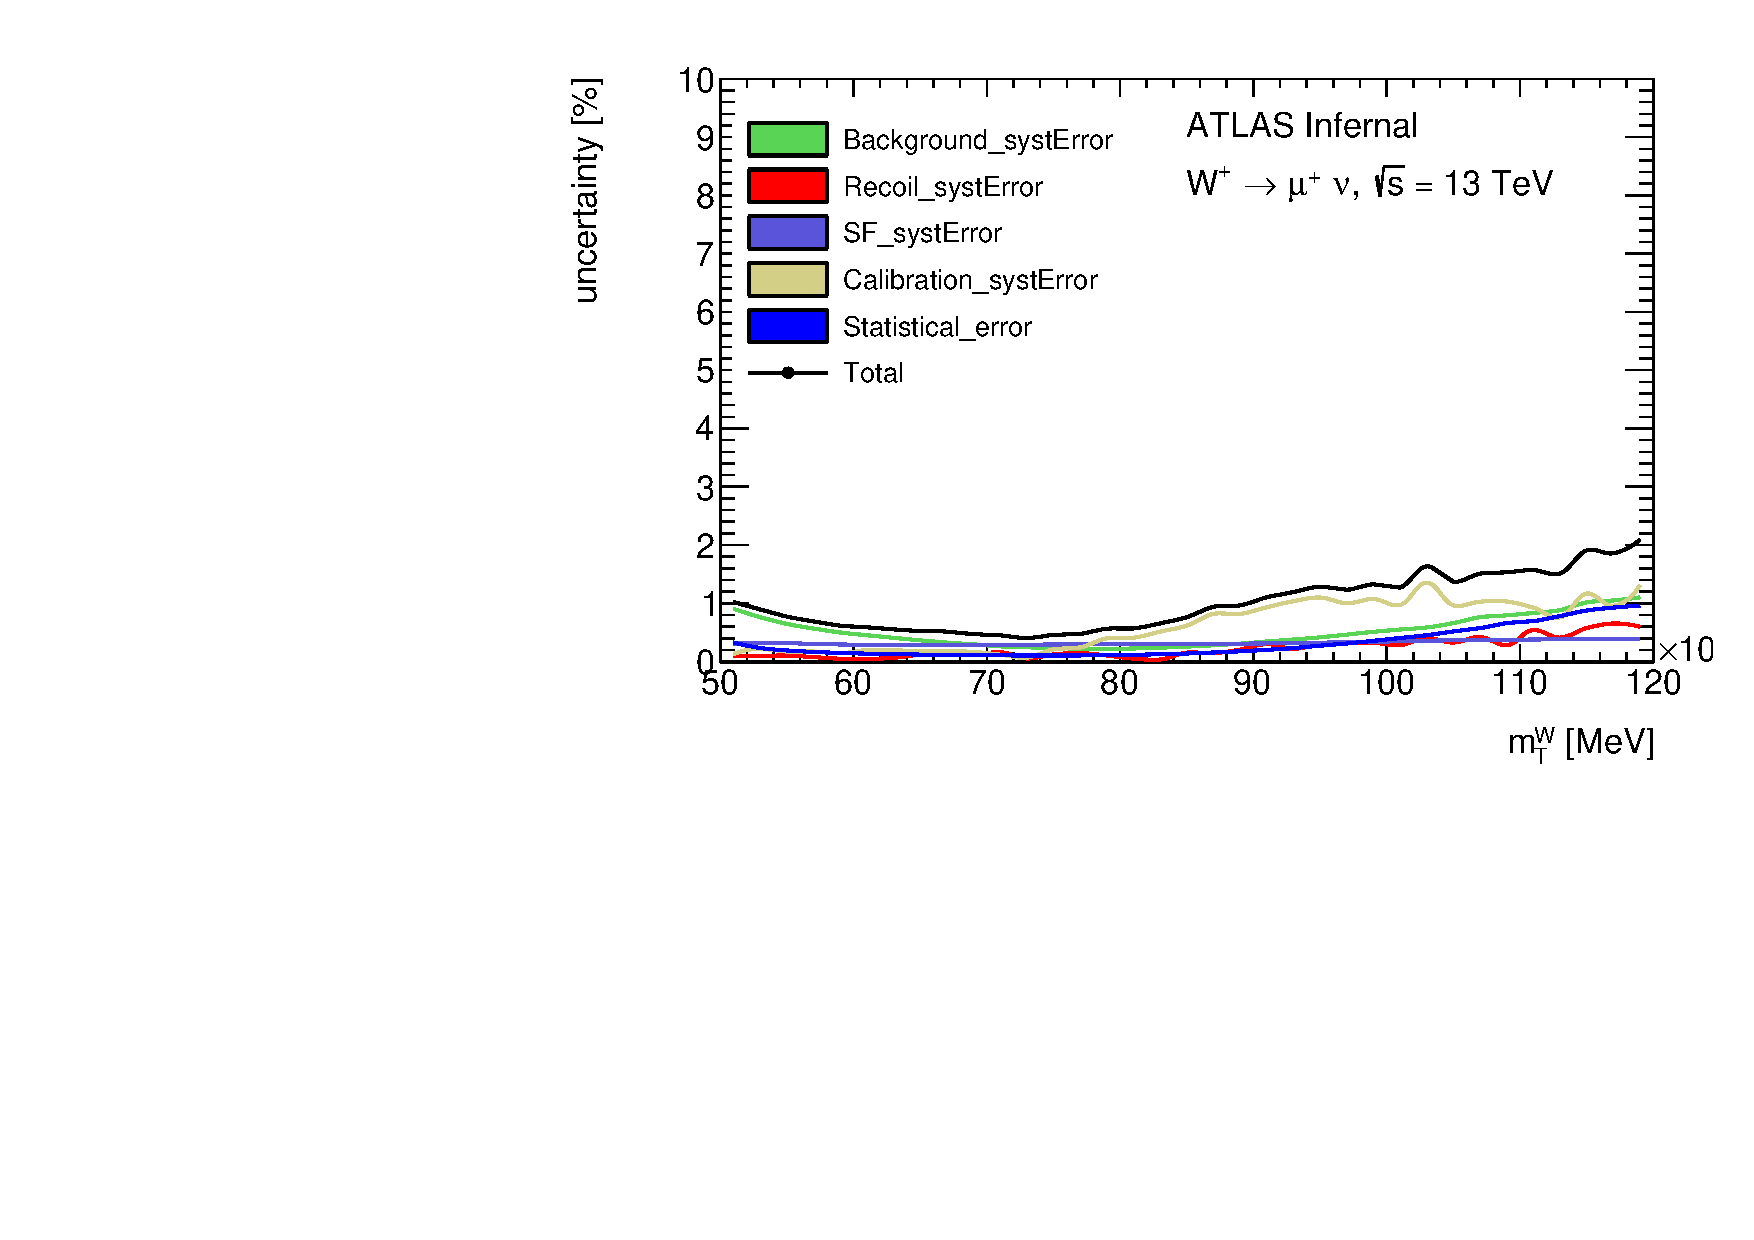
\includegraphics[width=.49\textwidth]{errors_mT_cut7_plusmunu_13TeV__NormErr.pdf}\label{f:}}
	
	{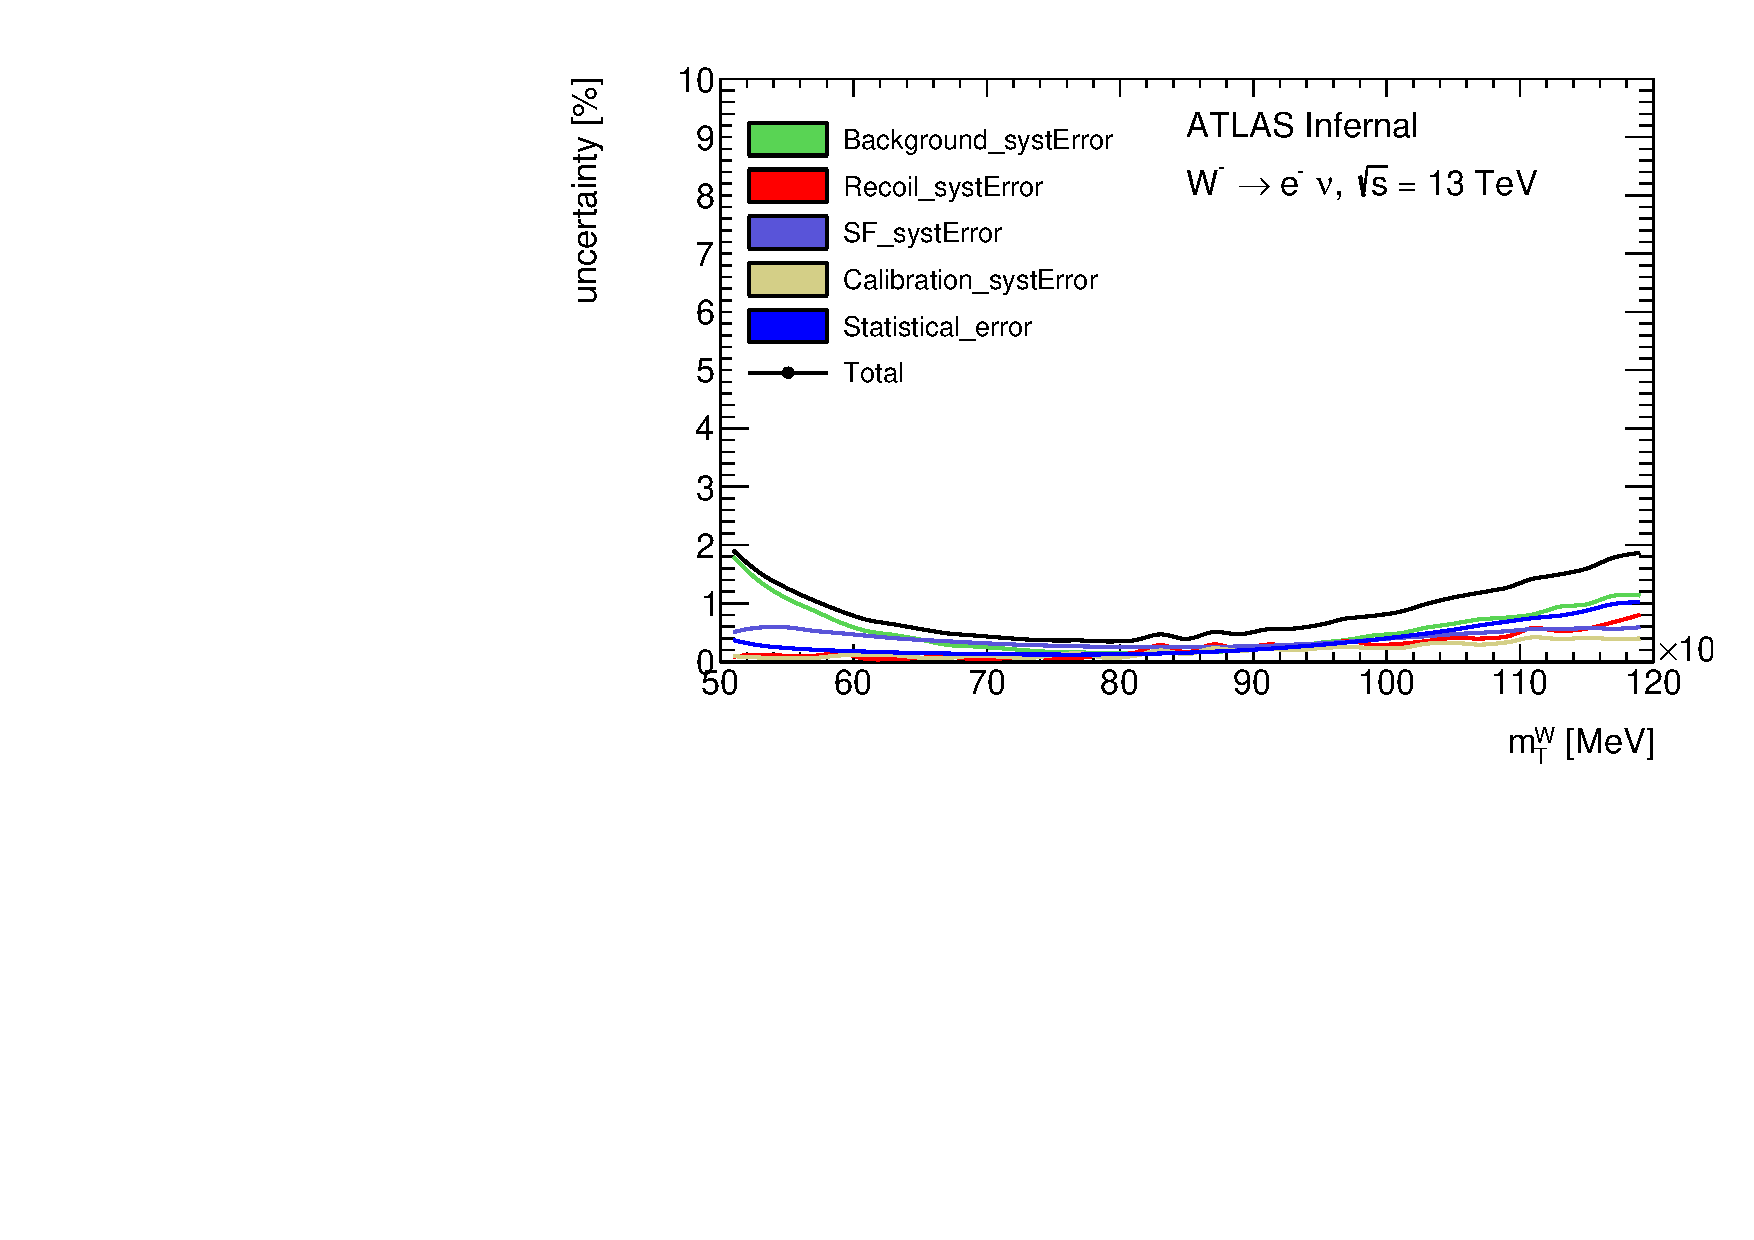
\includegraphics[width=.49\textwidth]{errors_mT_cut7_minusenu_13TeV__NormErr.pdf}\label{f:}}
	{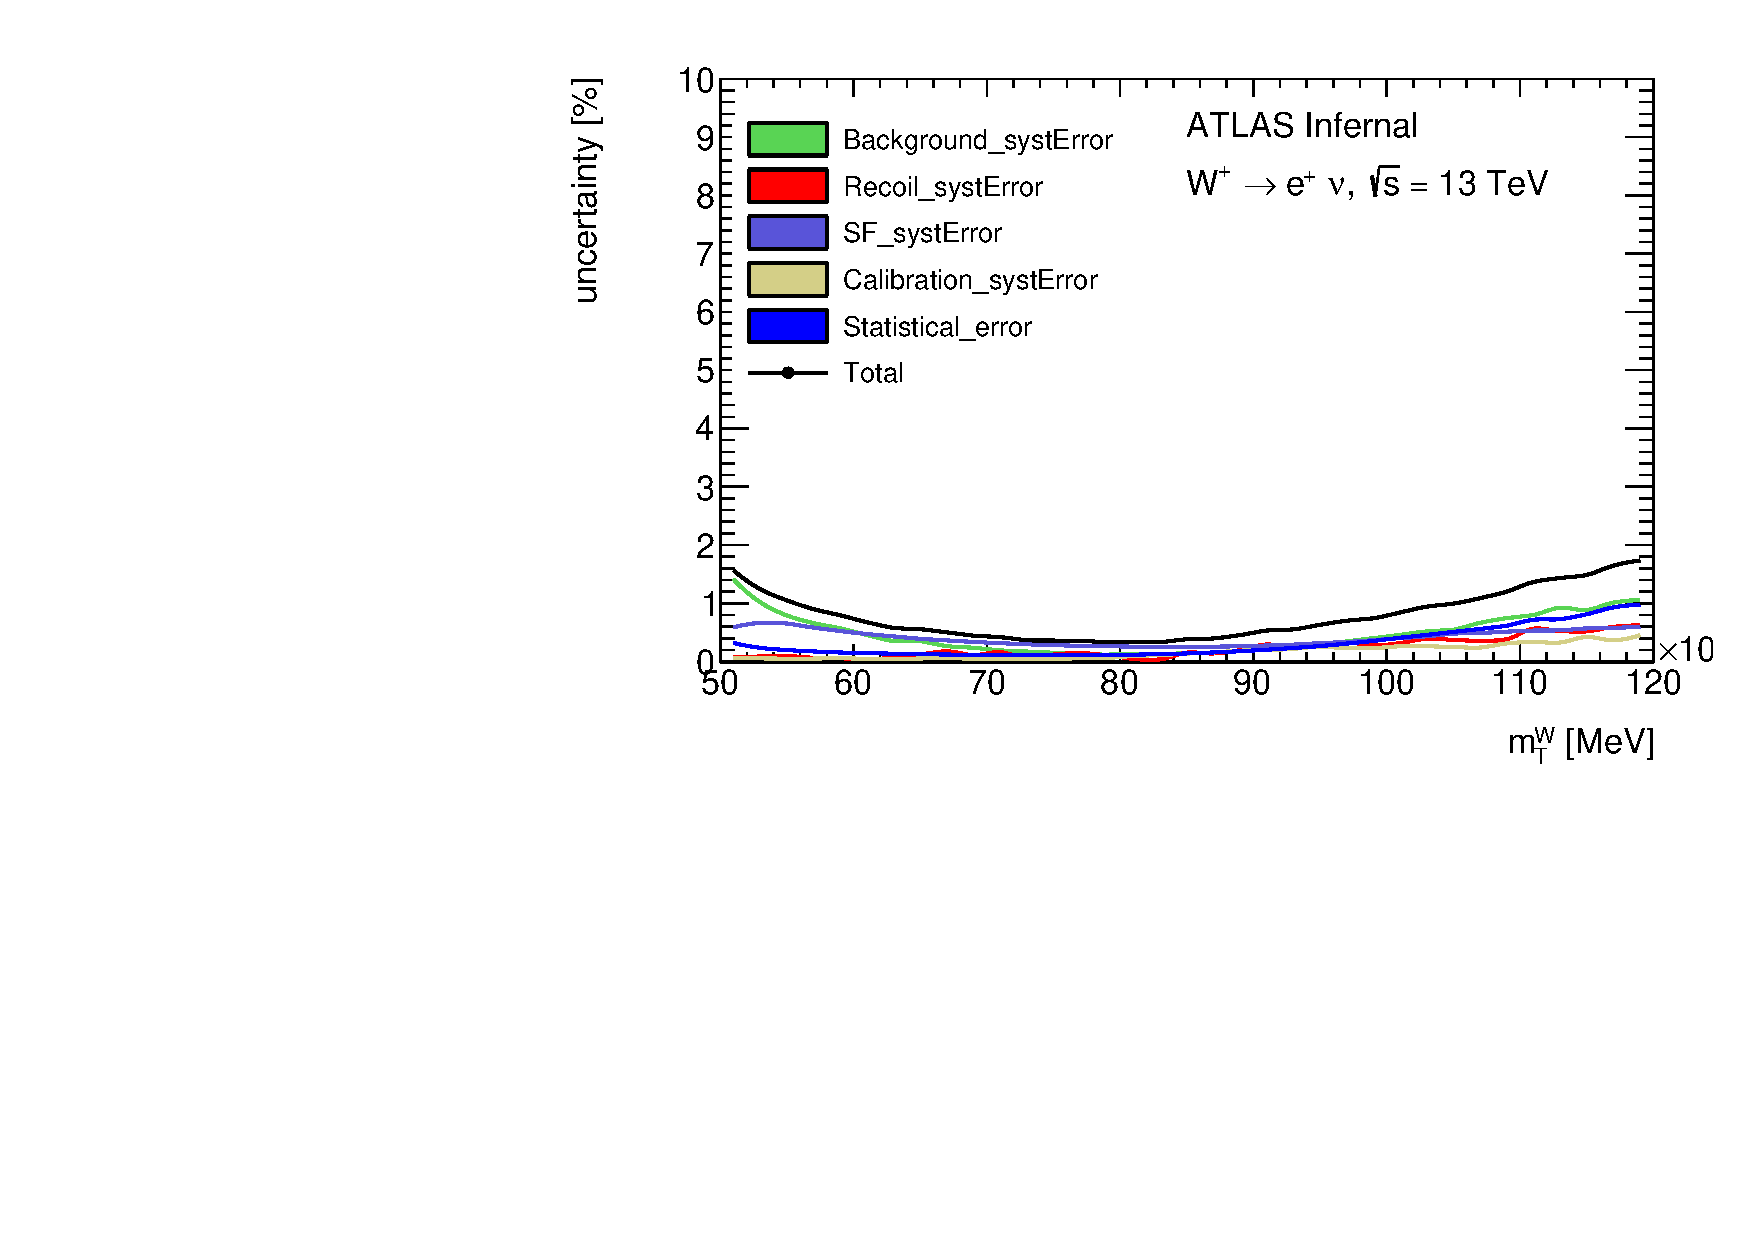
\includegraphics[width=.49\textwidth]{errors_mT_cut7_plusenu_13TeV__NormErr.pdf}\label{f:}}
	
	\caption{  Transverse mass systematic error breakdown of the W boson in the muon and electron channel  for the $\sqrt{s} = 5$~\TeV\ and $\sqrt{s} = 13$~\TeV\ datasets.} \end{figure}
\newpage

\begin{figure}[h]
	\centering
	{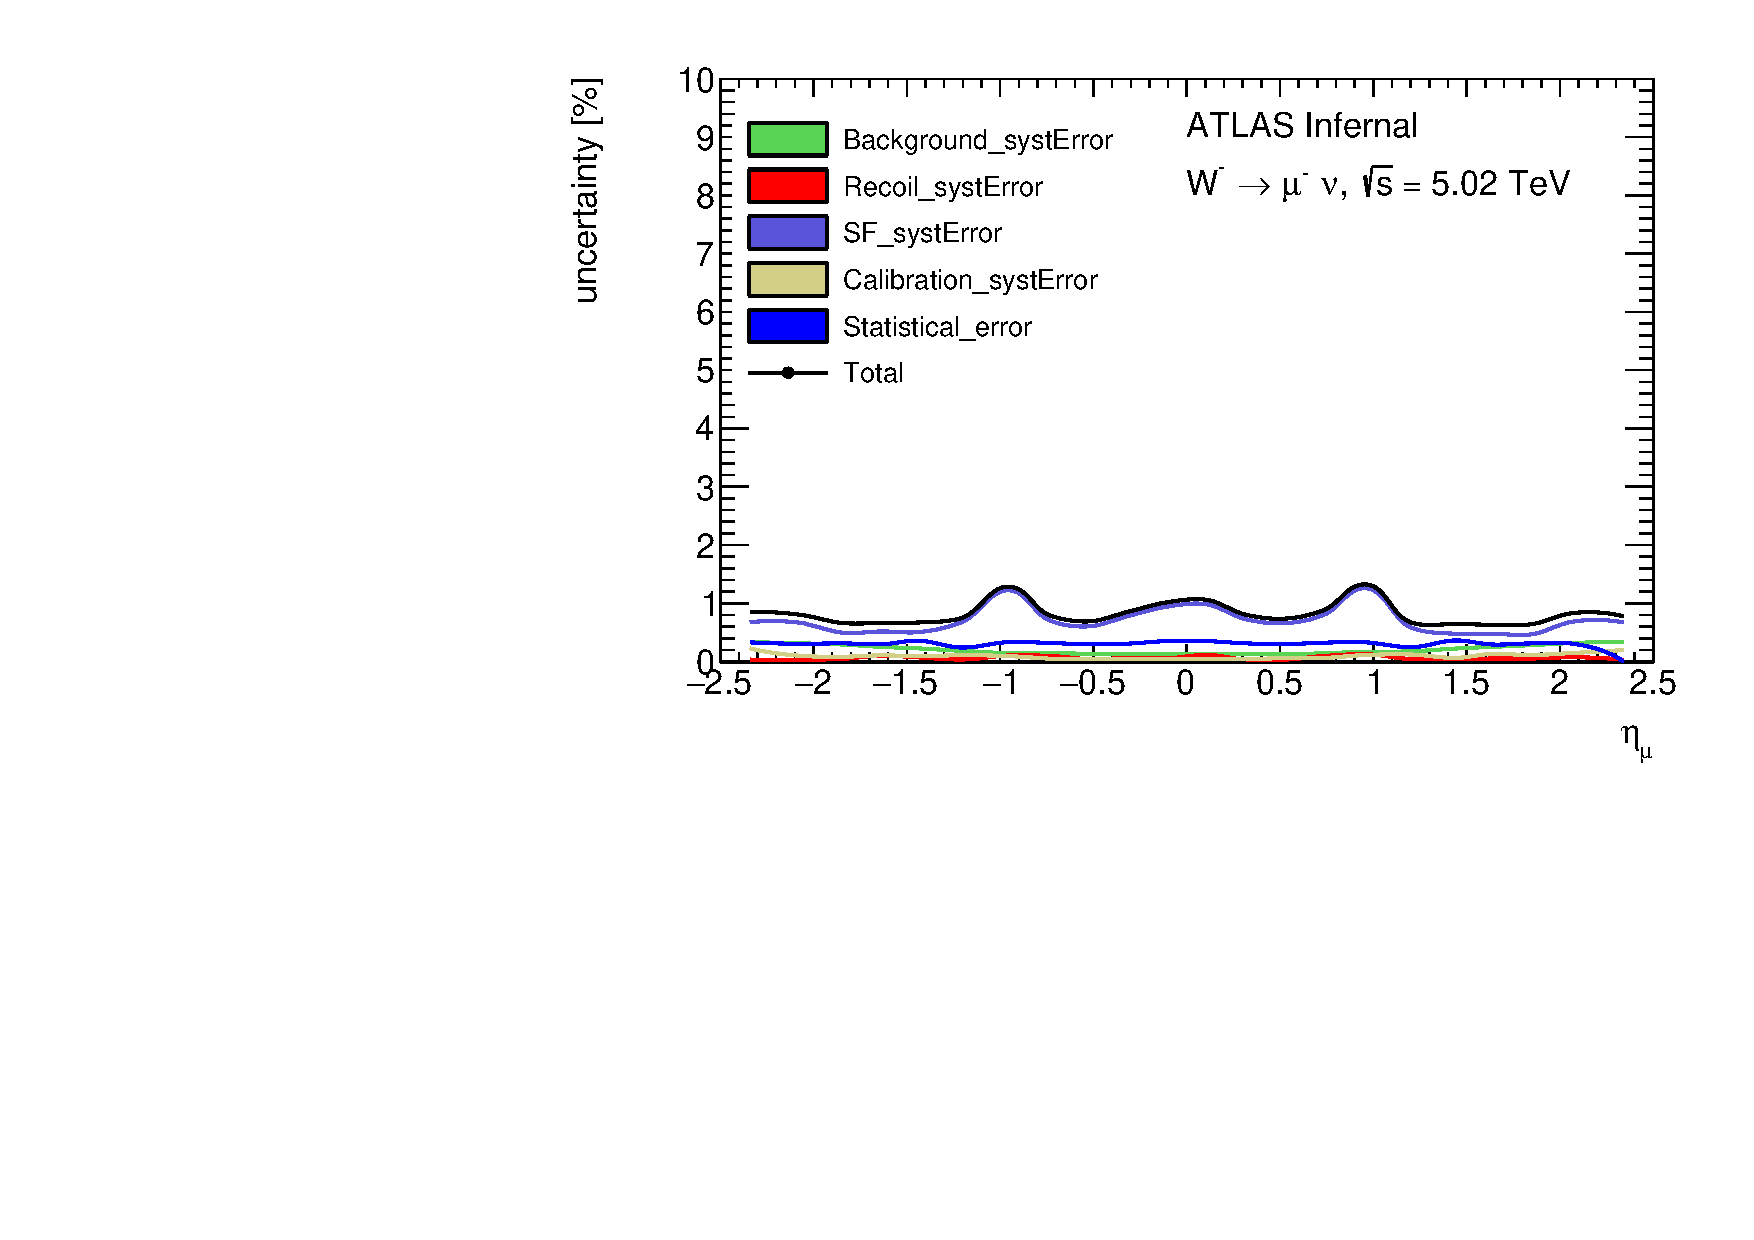
\includegraphics[width=.49\textwidth]{errors_muEta_cut7_minusmunu_5TeV__NormErr.pdf}\label{f:}}
	{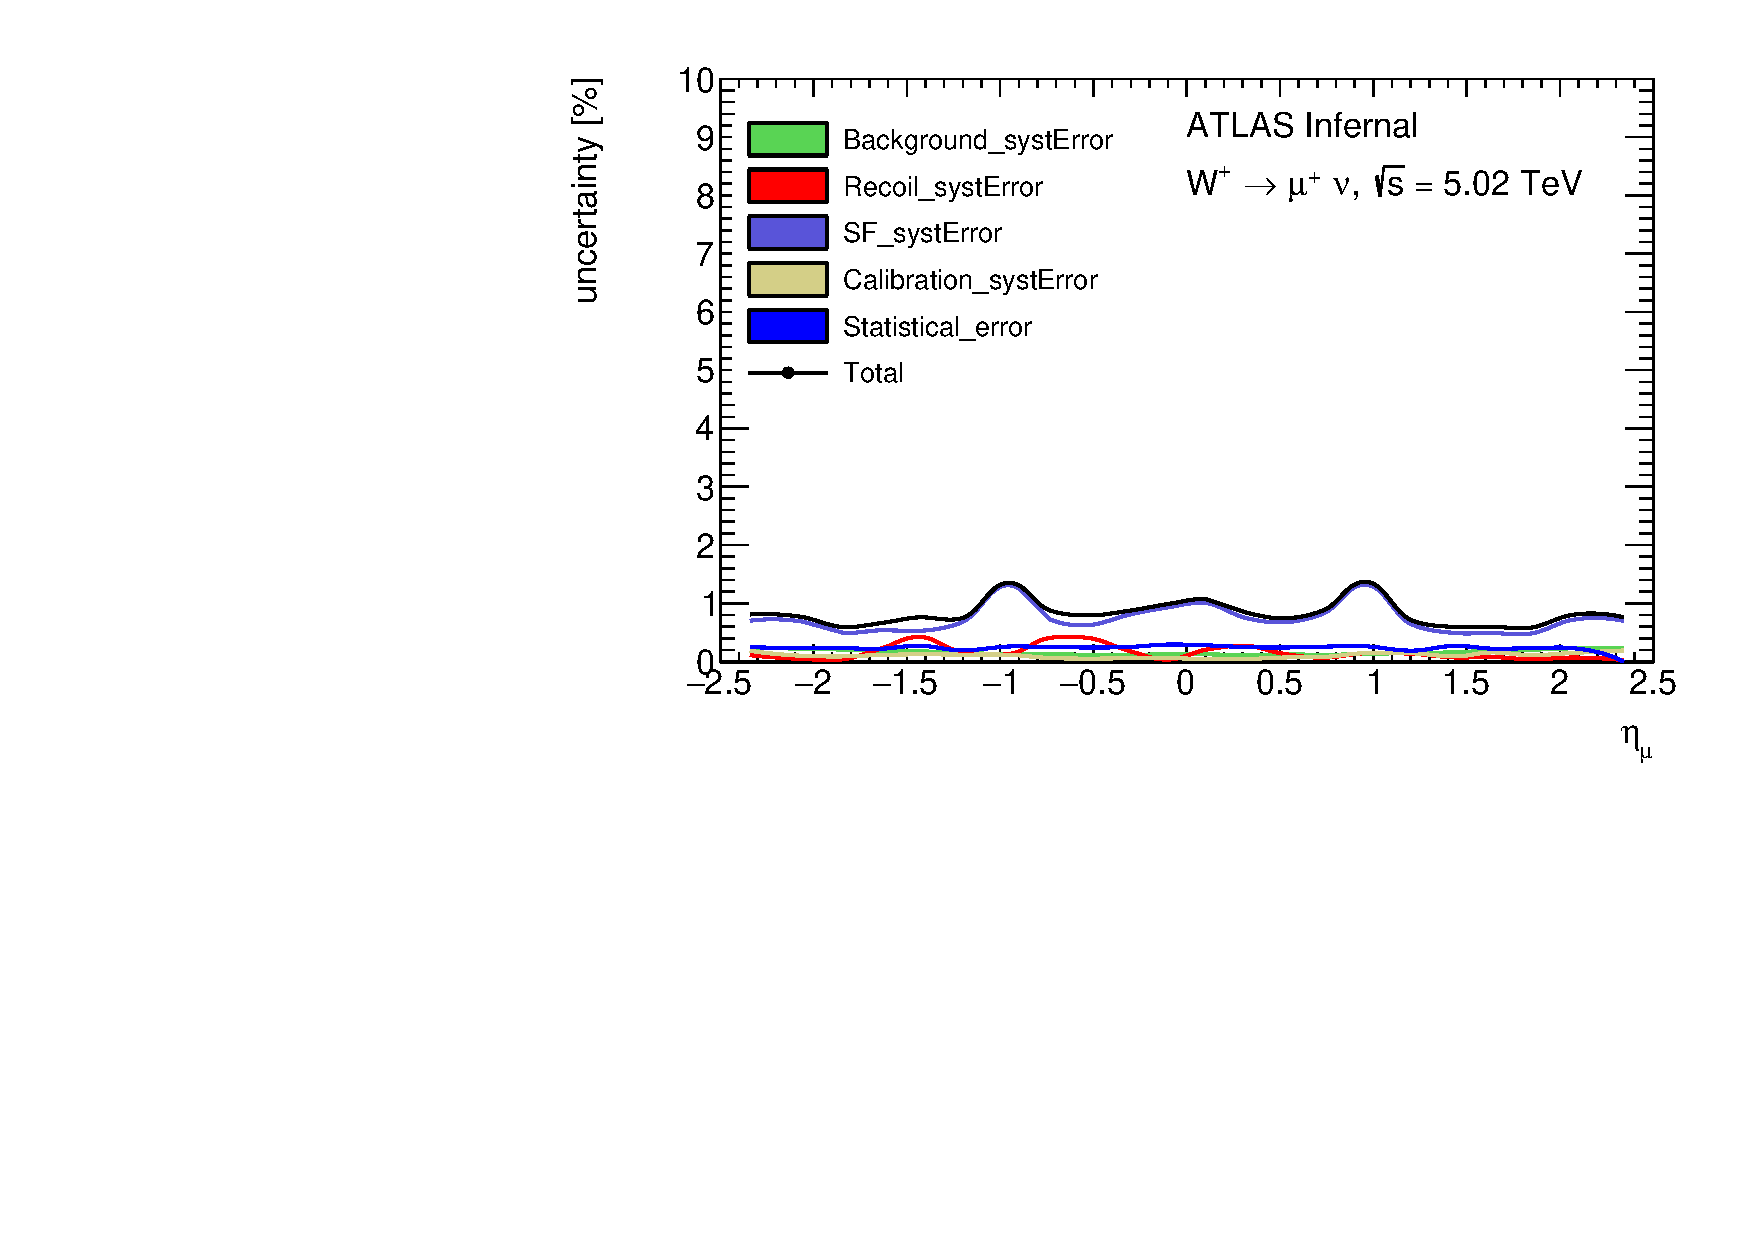
\includegraphics[width=.49\textwidth]{errors_muEta_cut7_plusmunu_5TeV__NormErr.pdf}\label{f:}}
	
	{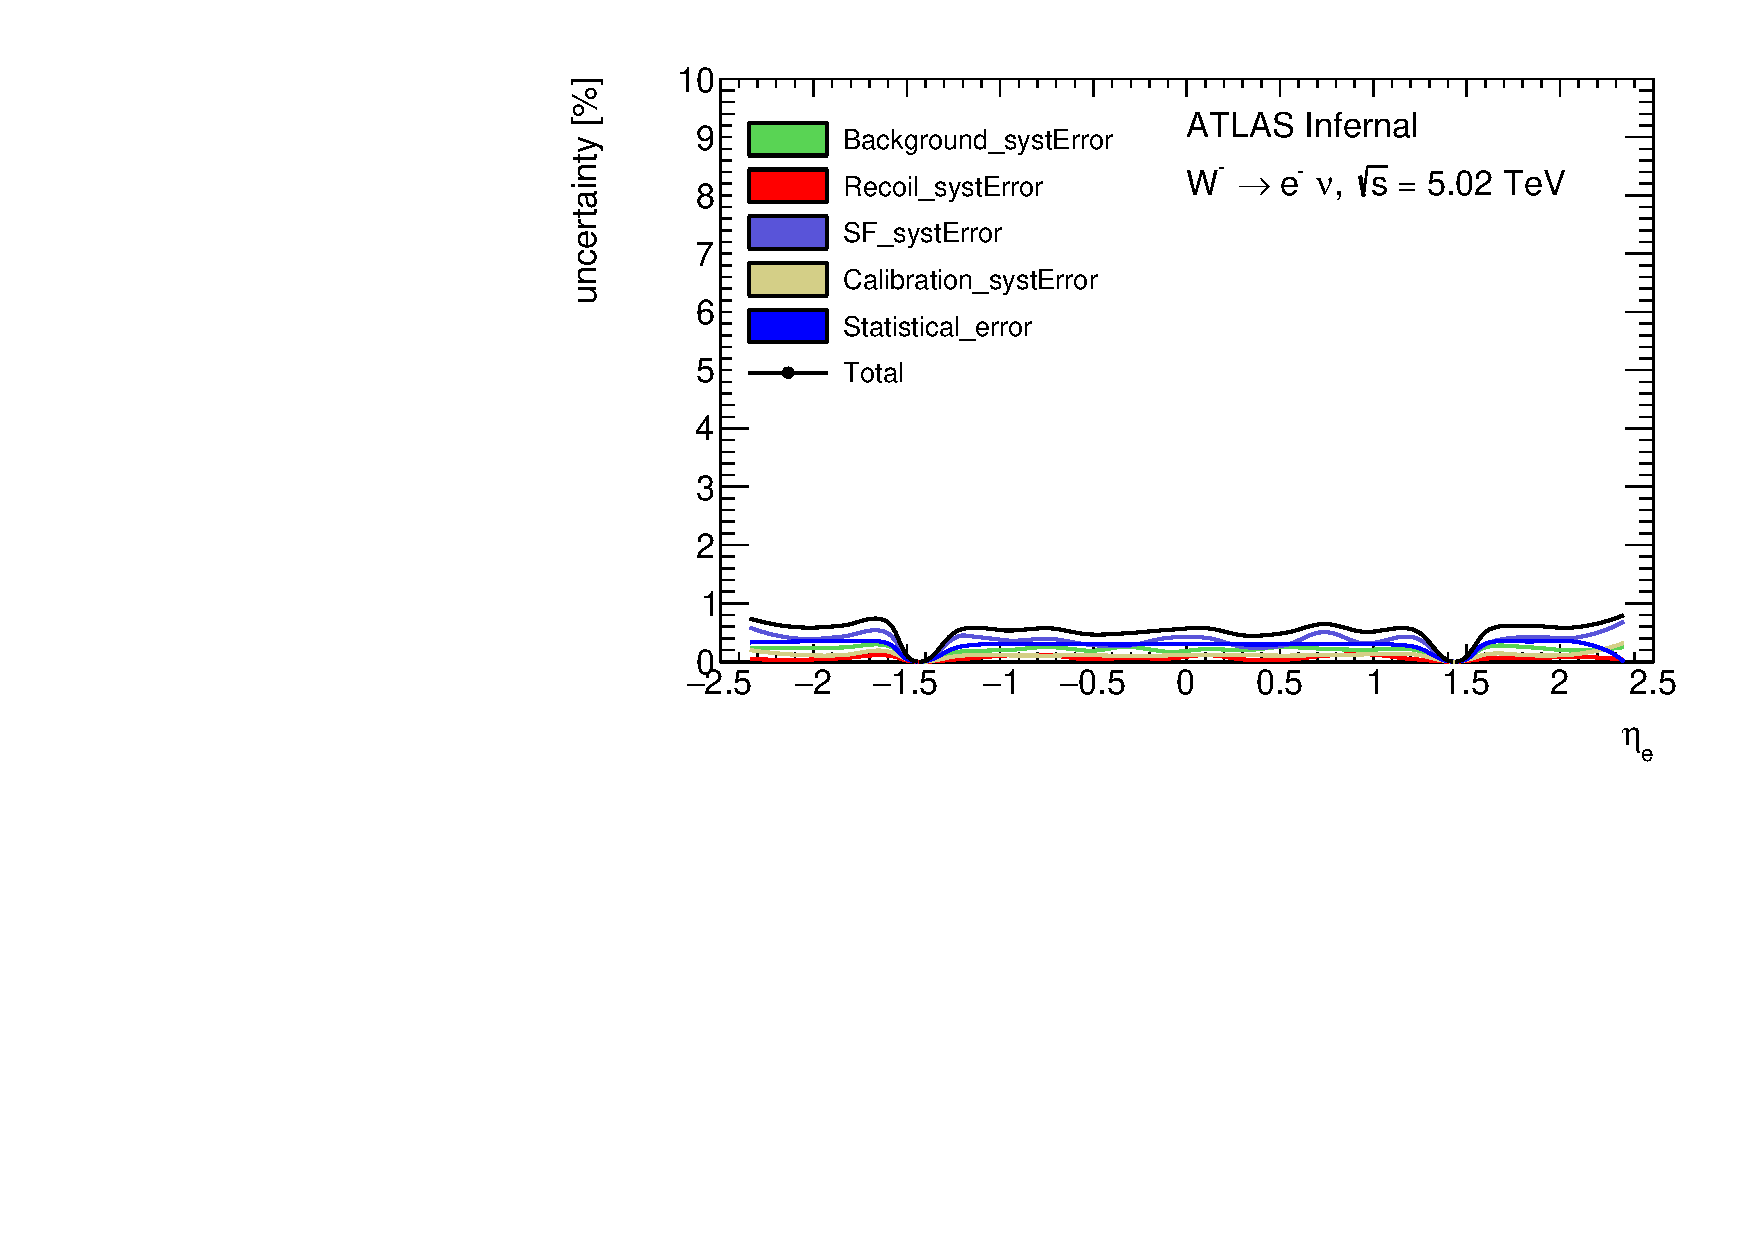
\includegraphics[width=.49\textwidth]{errors_elEta_cut7_minusenu_5TeV__NormErr.pdf}\label{f:}}
	{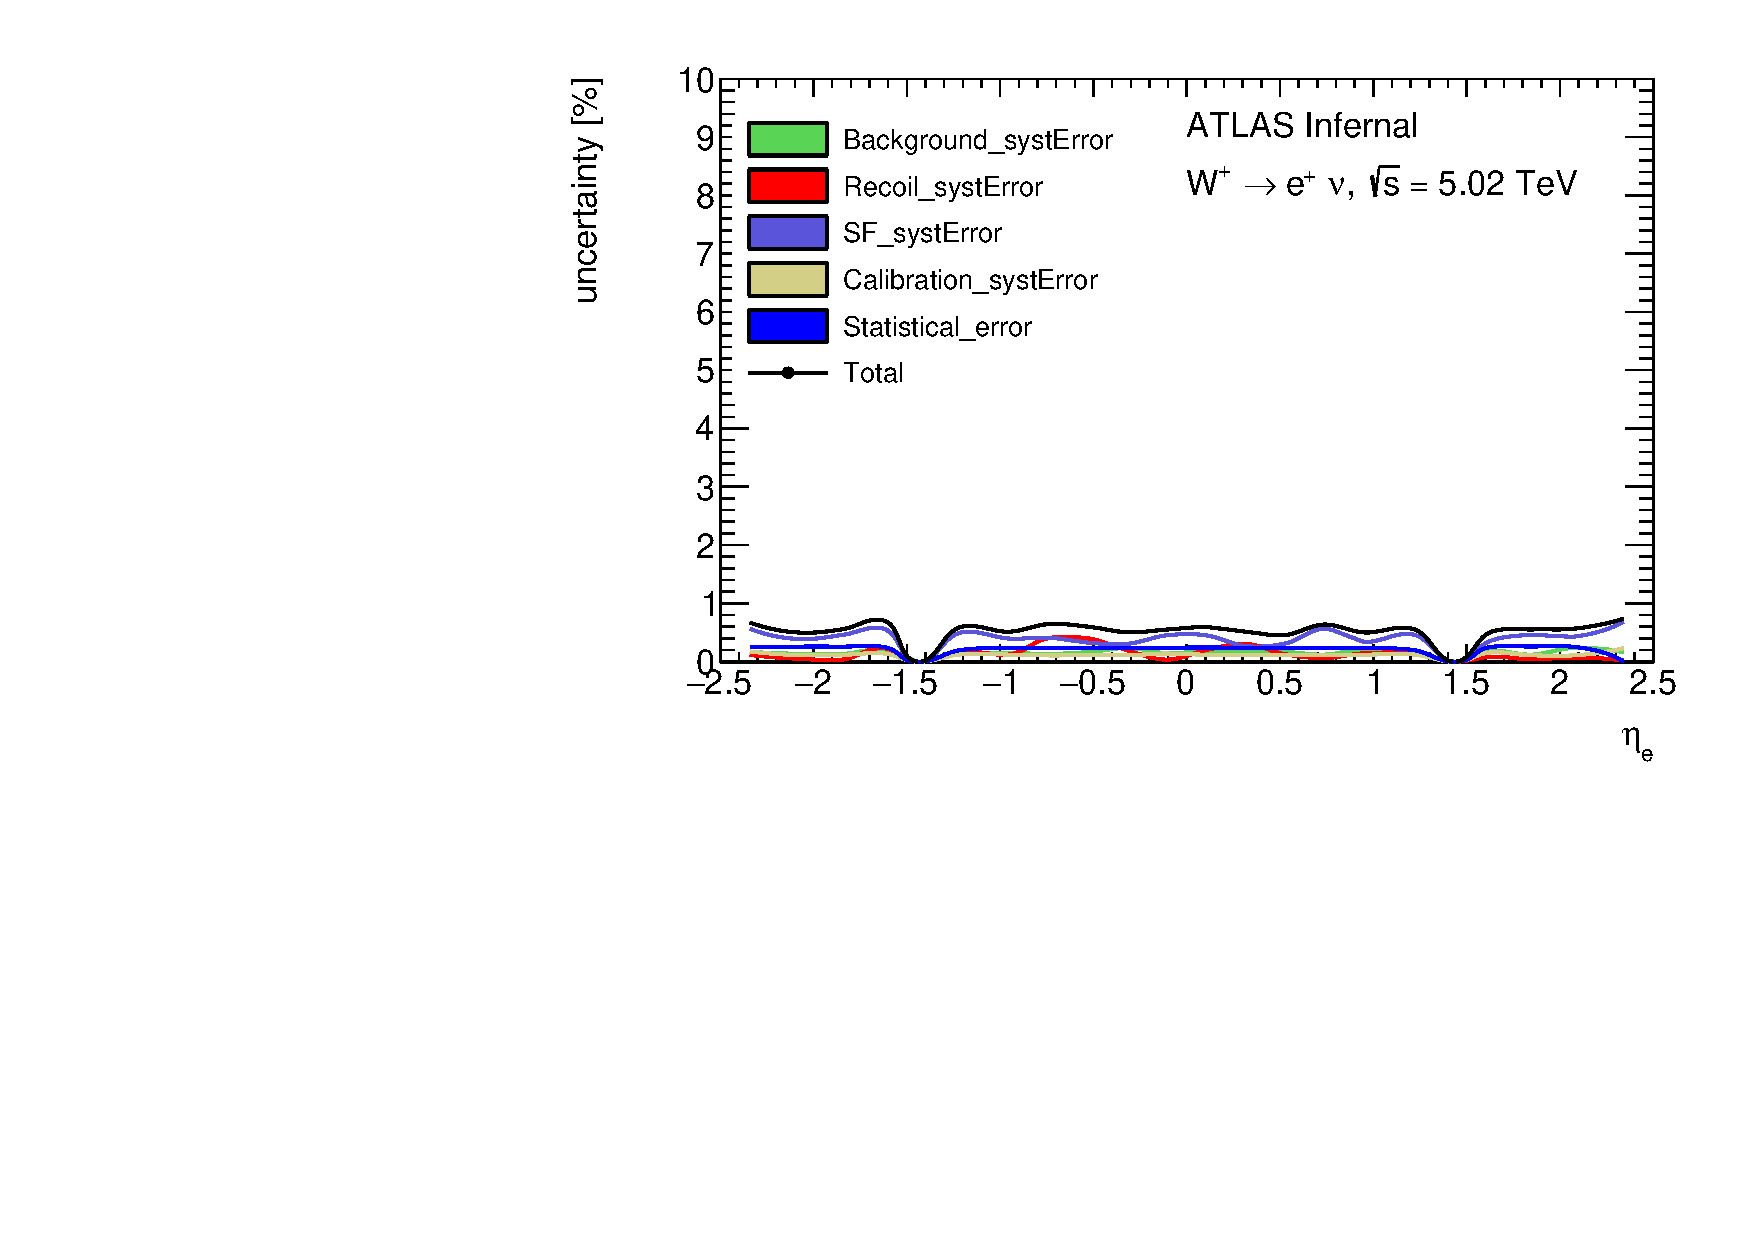
\includegraphics[width=.49\textwidth]{errors_elEta_cut7_plusenu_5TeV__NormErr.pdf}\label{f:}}
	
		{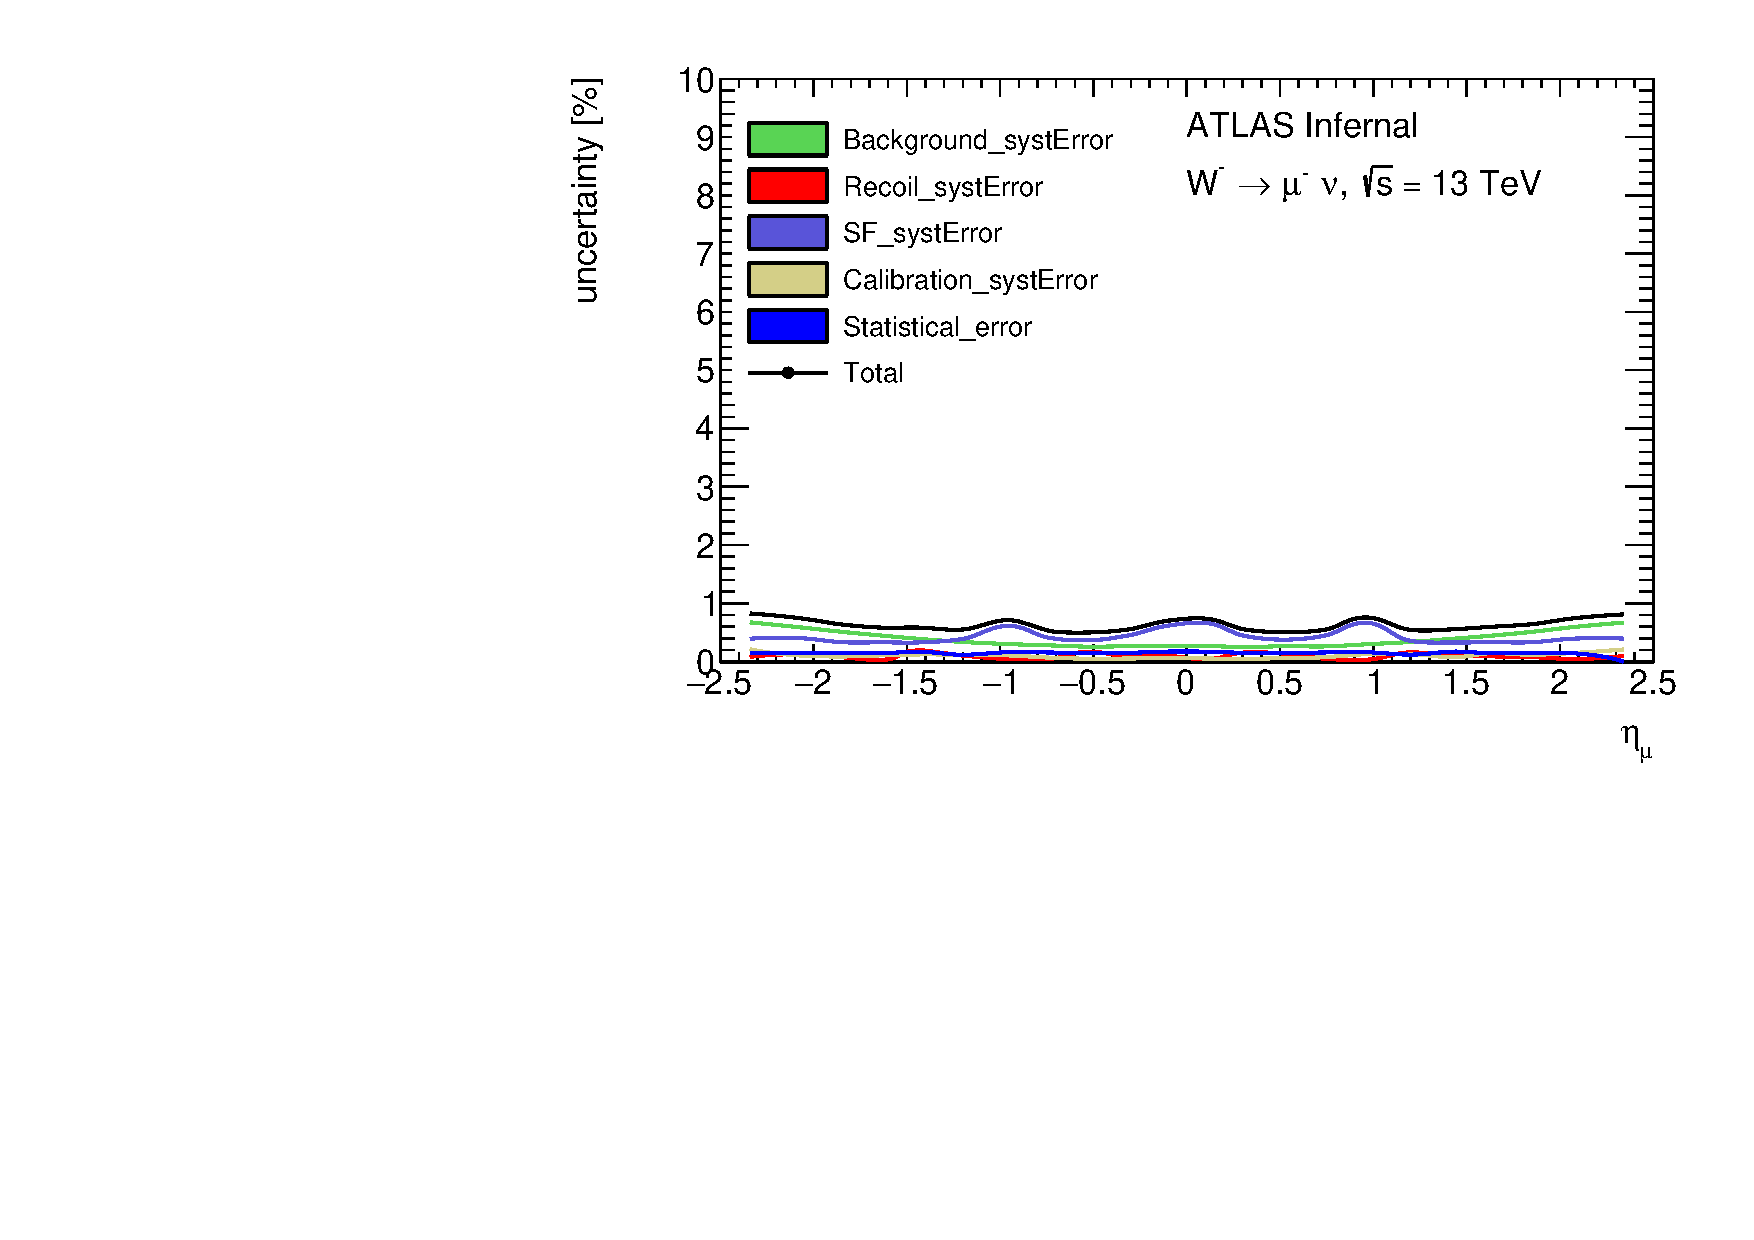
\includegraphics[width=.49\textwidth]{errors_muEta_cut7_minusmunu_13TeV__NormErr.pdf}\label{f:}}
	{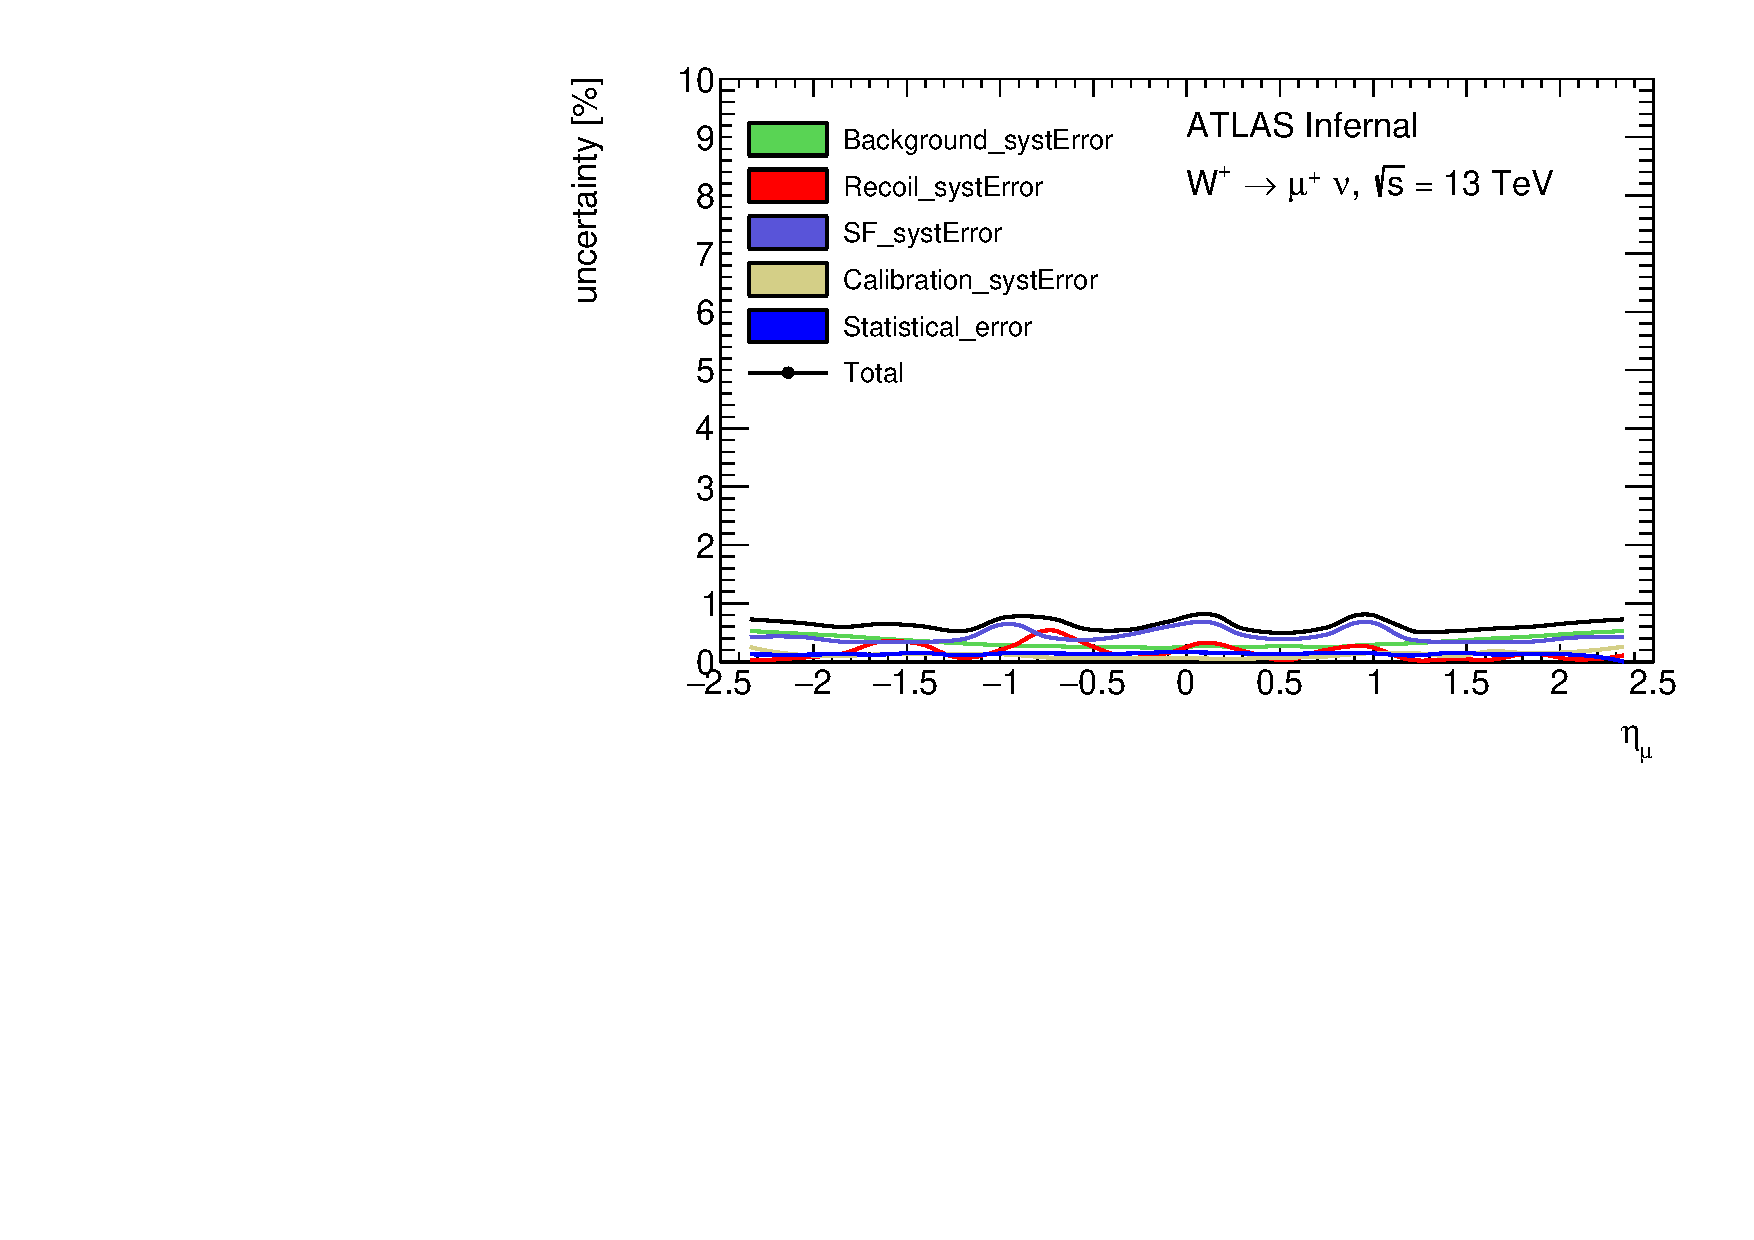
\includegraphics[width=.49\textwidth]{errors_muEta_cut7_plusmunu_13TeV__NormErr.pdf}\label{f:}}
	
	{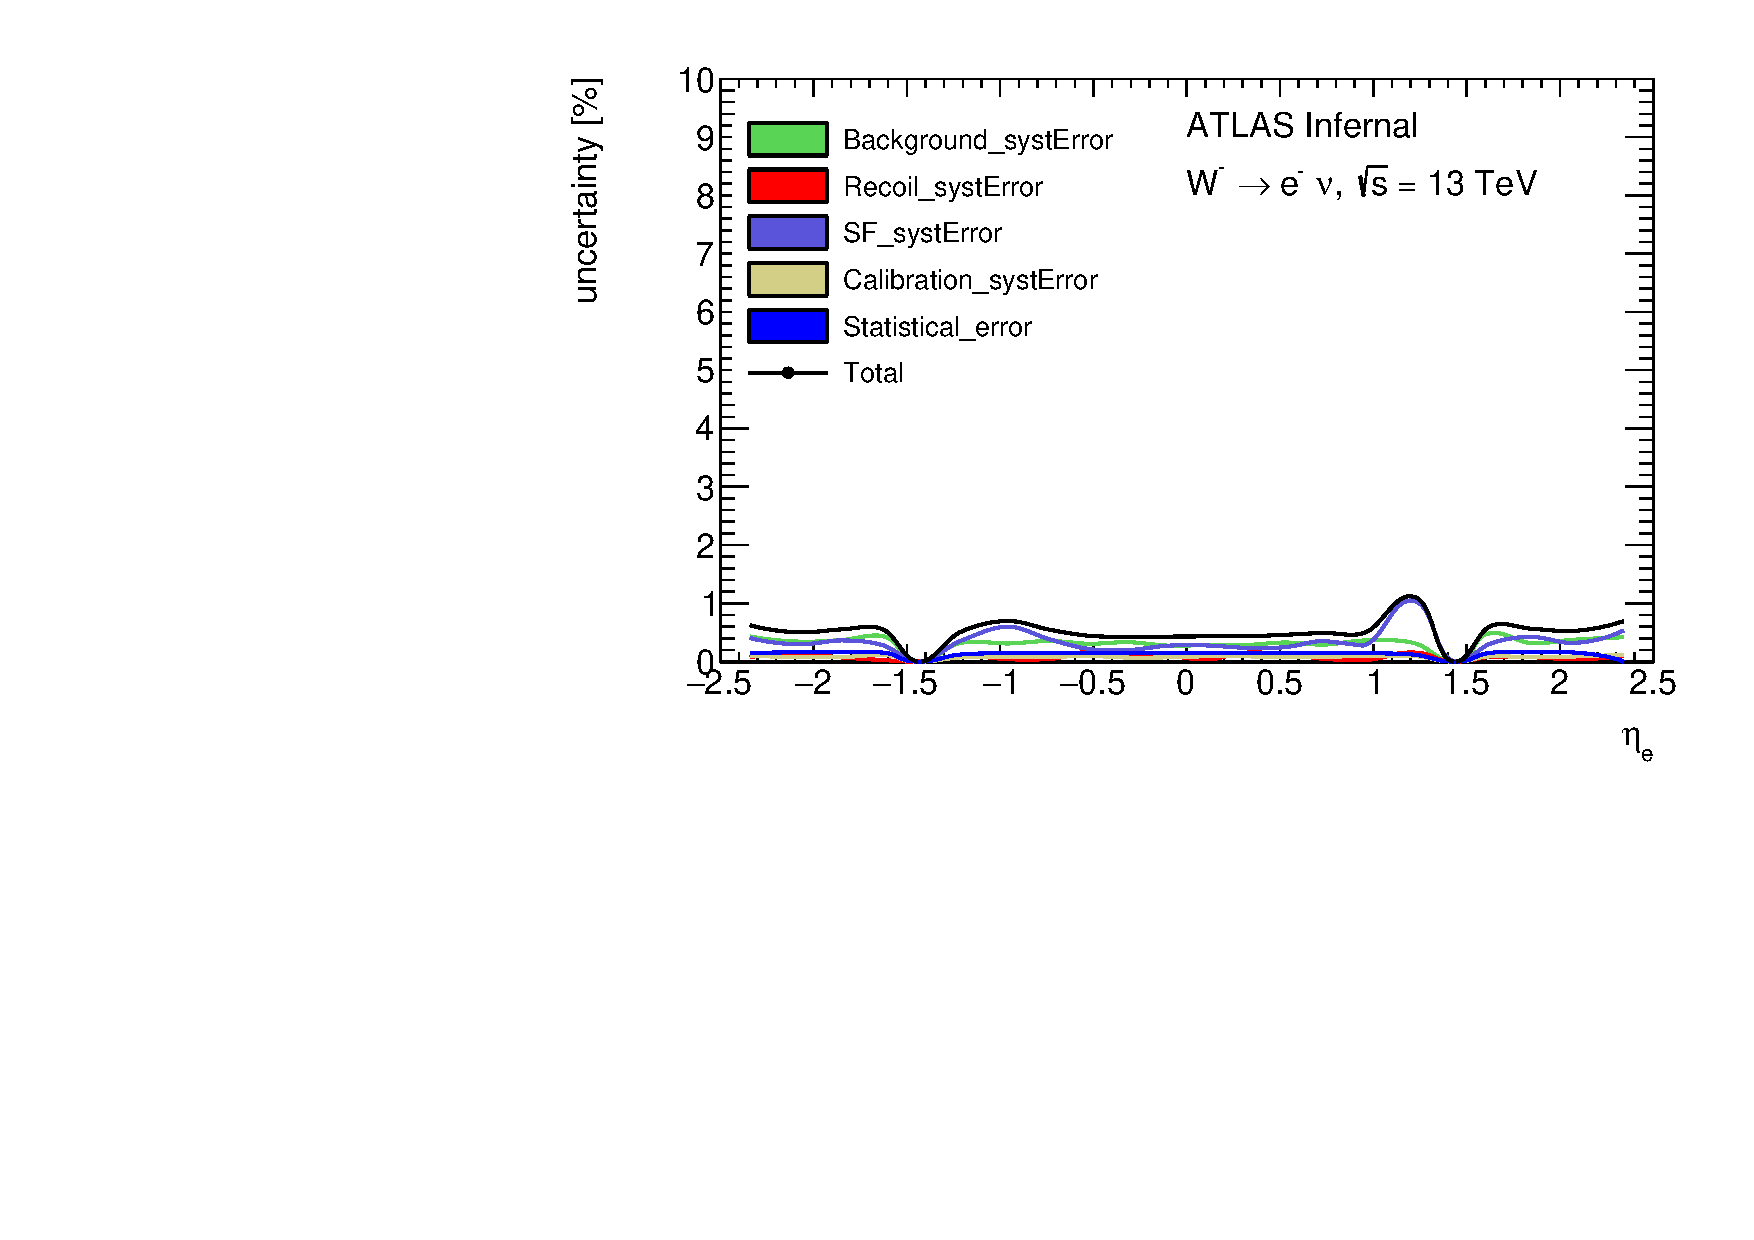
\includegraphics[width=.49\textwidth]{errors_elEta_cut7_minusenu_13TeV__NormErr.pdf}\label{f:}}
	{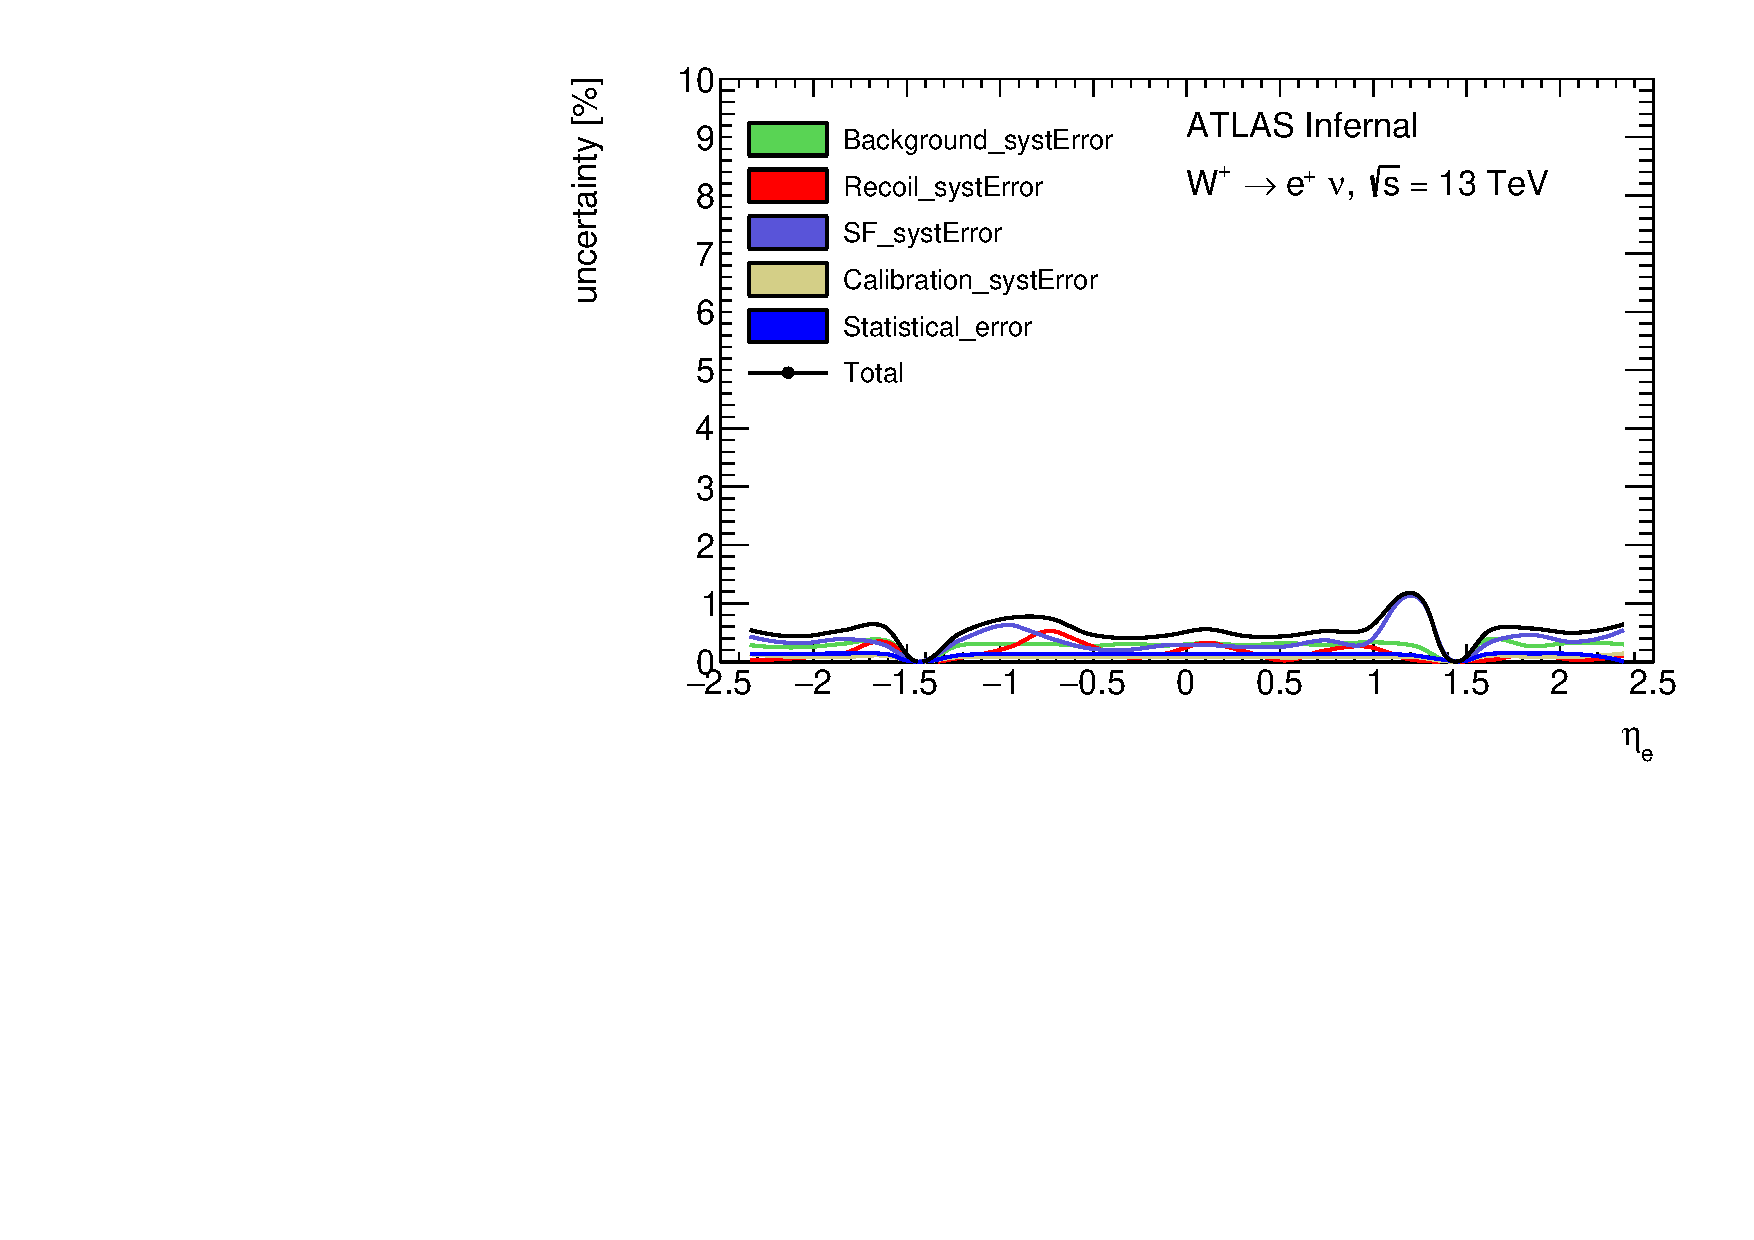
\includegraphics[width=.49\textwidth]{errors_elEta_cut7_plusenu_13TeV__NormErr.pdf}\label{f:}}
	\caption{  Lepton pseudorapidity systematic error breakdown in the muon and electron channel  for the $\sqrt{s} = 5$~\TeV\ and $\sqrt{s} = 13$~\TeV\ datasets.}
\end{figure}
\newpage

\begin{figure}[h]
	\centering
	{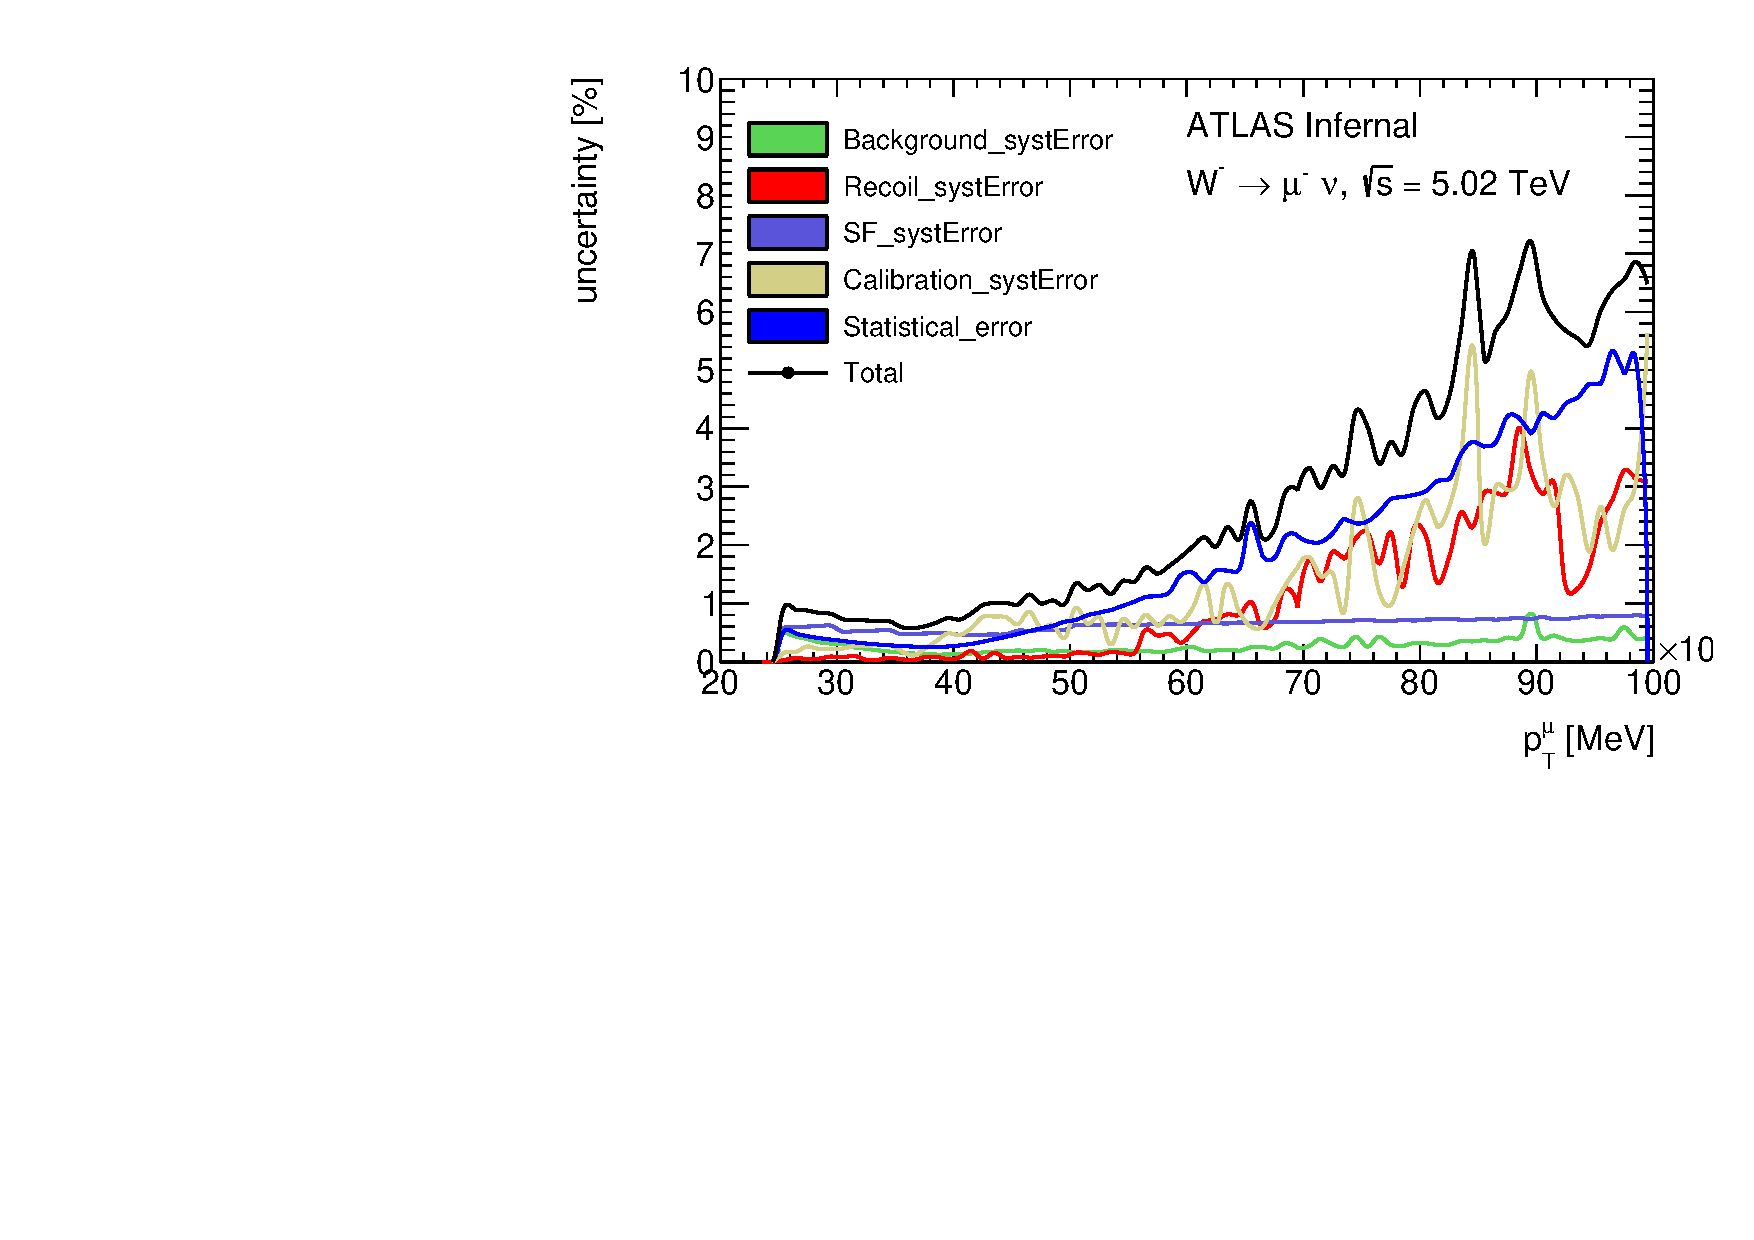
\includegraphics[width=.49\textwidth]{errors_muPt_cut7_minusmunu_5TeV__NormErr.pdf}\label{f:}}
	{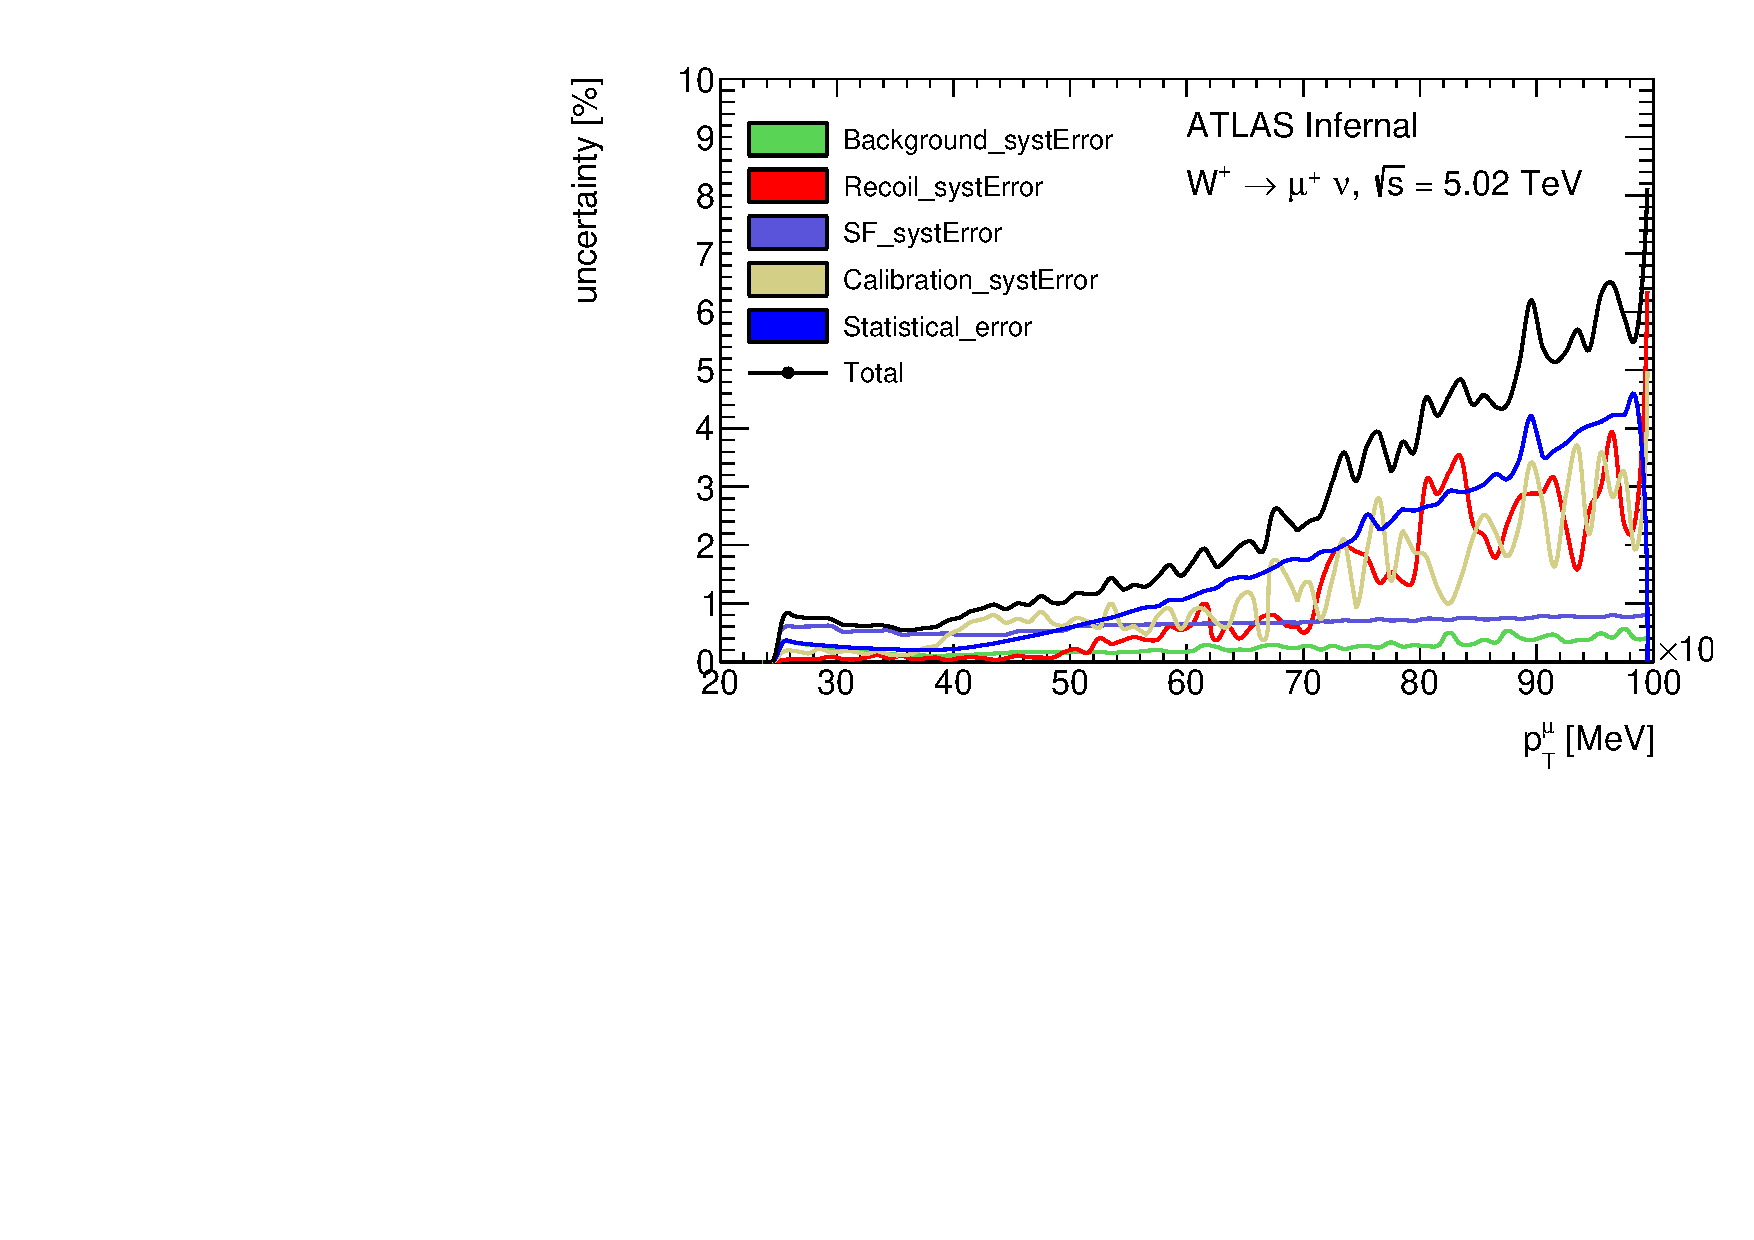
\includegraphics[width=.49\textwidth]{errors_muPt_cut7_plusmunu_5TeV__NormErr.pdf}\label{f:}}
	
	{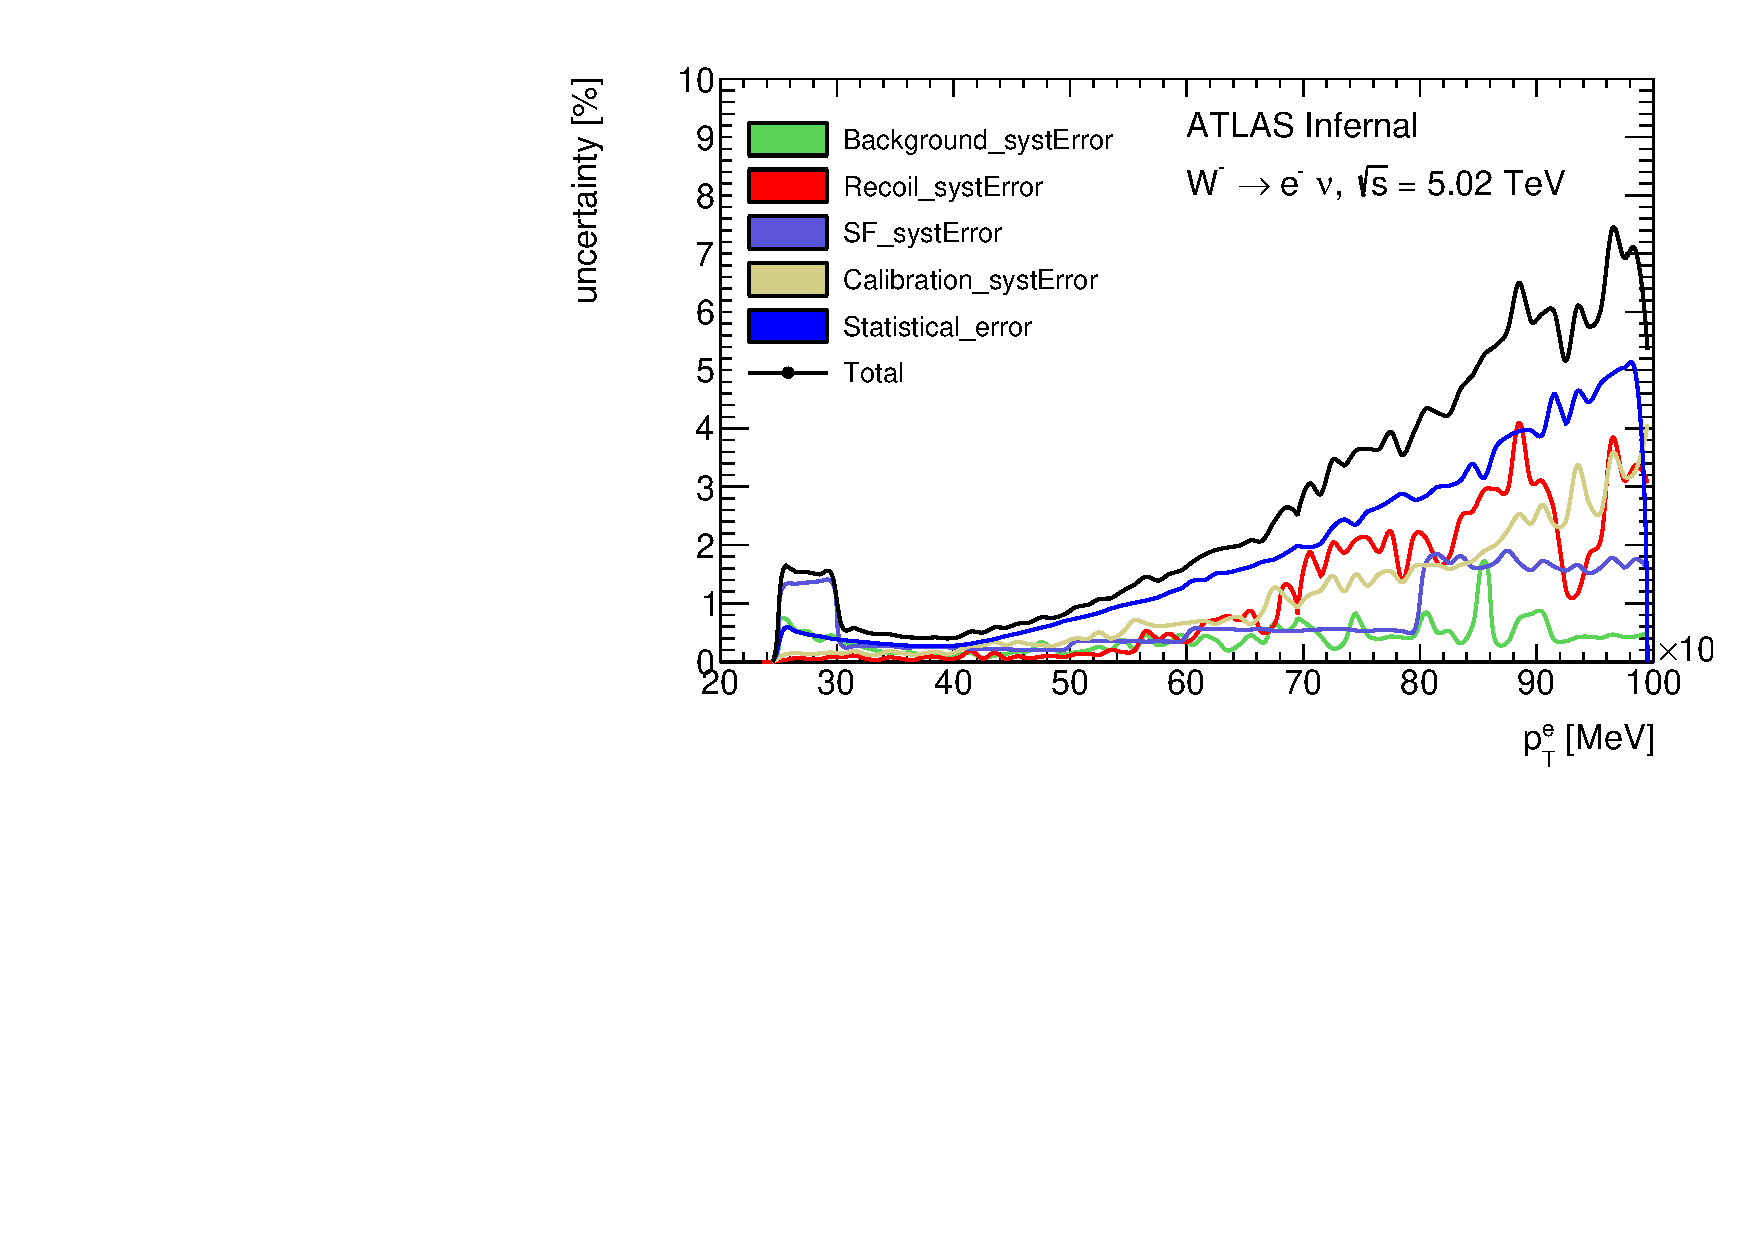
\includegraphics[width=.49\textwidth]{errors_elPt_cut7_minusenu_5TeV__NormErr.pdf}\label{f:}}
	{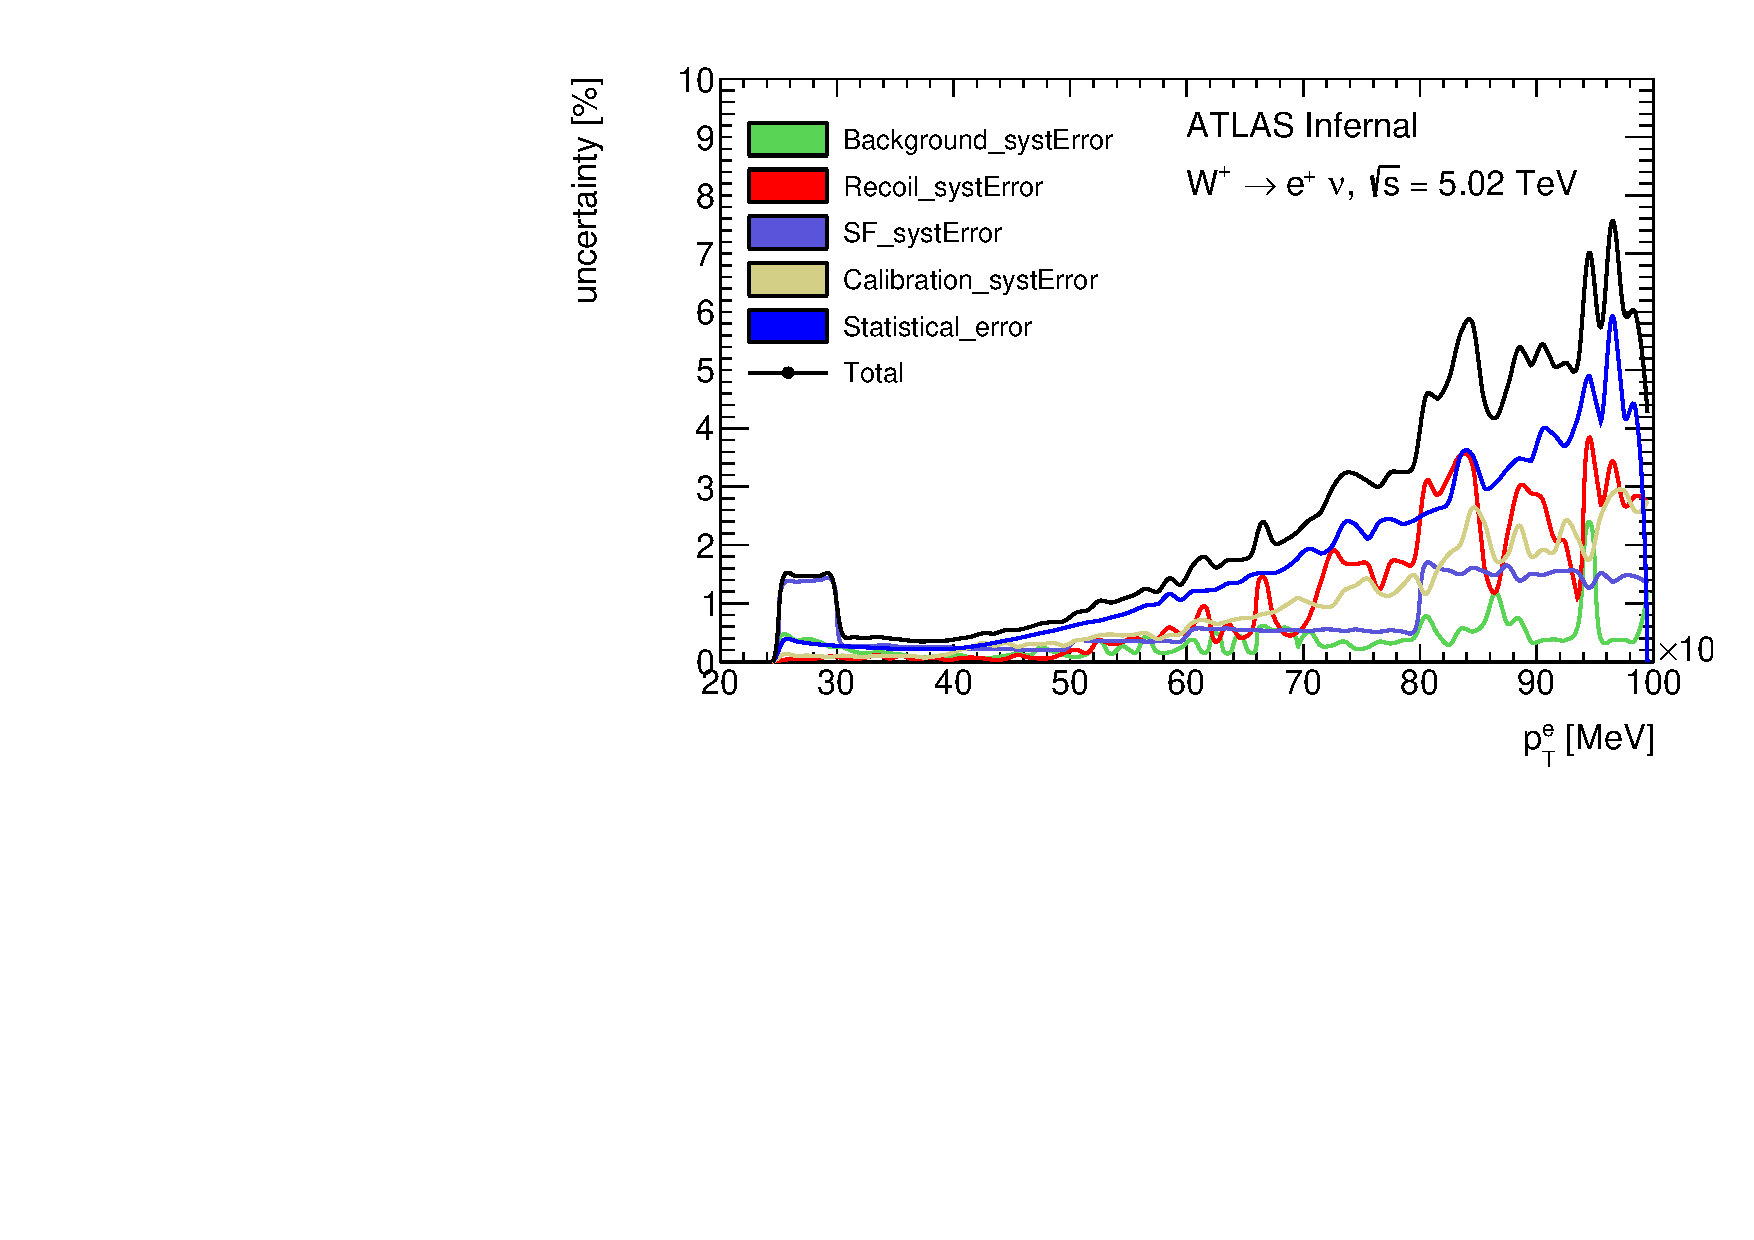
\includegraphics[width=.49\textwidth]{errors_elPt_cut7_plusenu_5TeV__NormErr.pdf}\label{f:}}
	
		{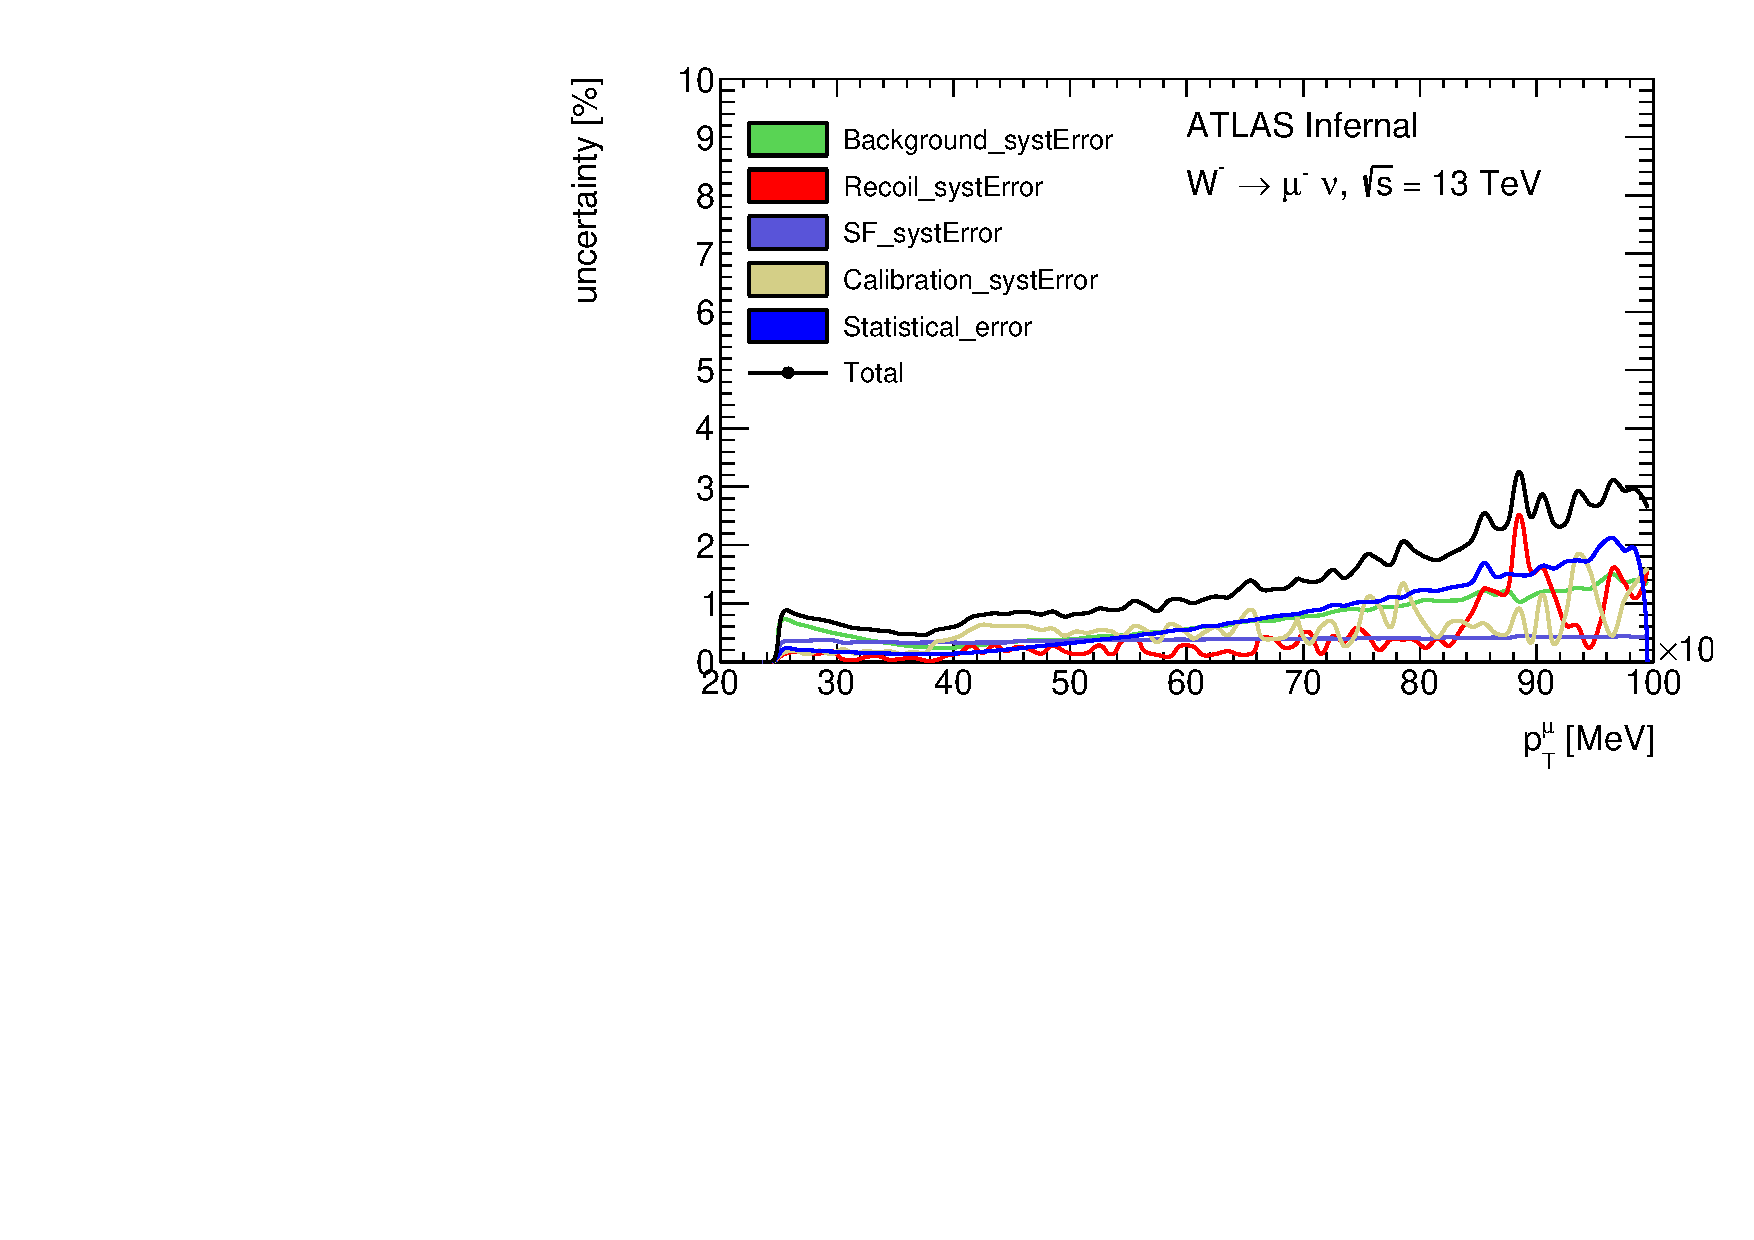
\includegraphics[width=.49\textwidth]{errors_muPt_cut7_minusmunu_13TeV__NormErr.pdf}\label{f:}}
	{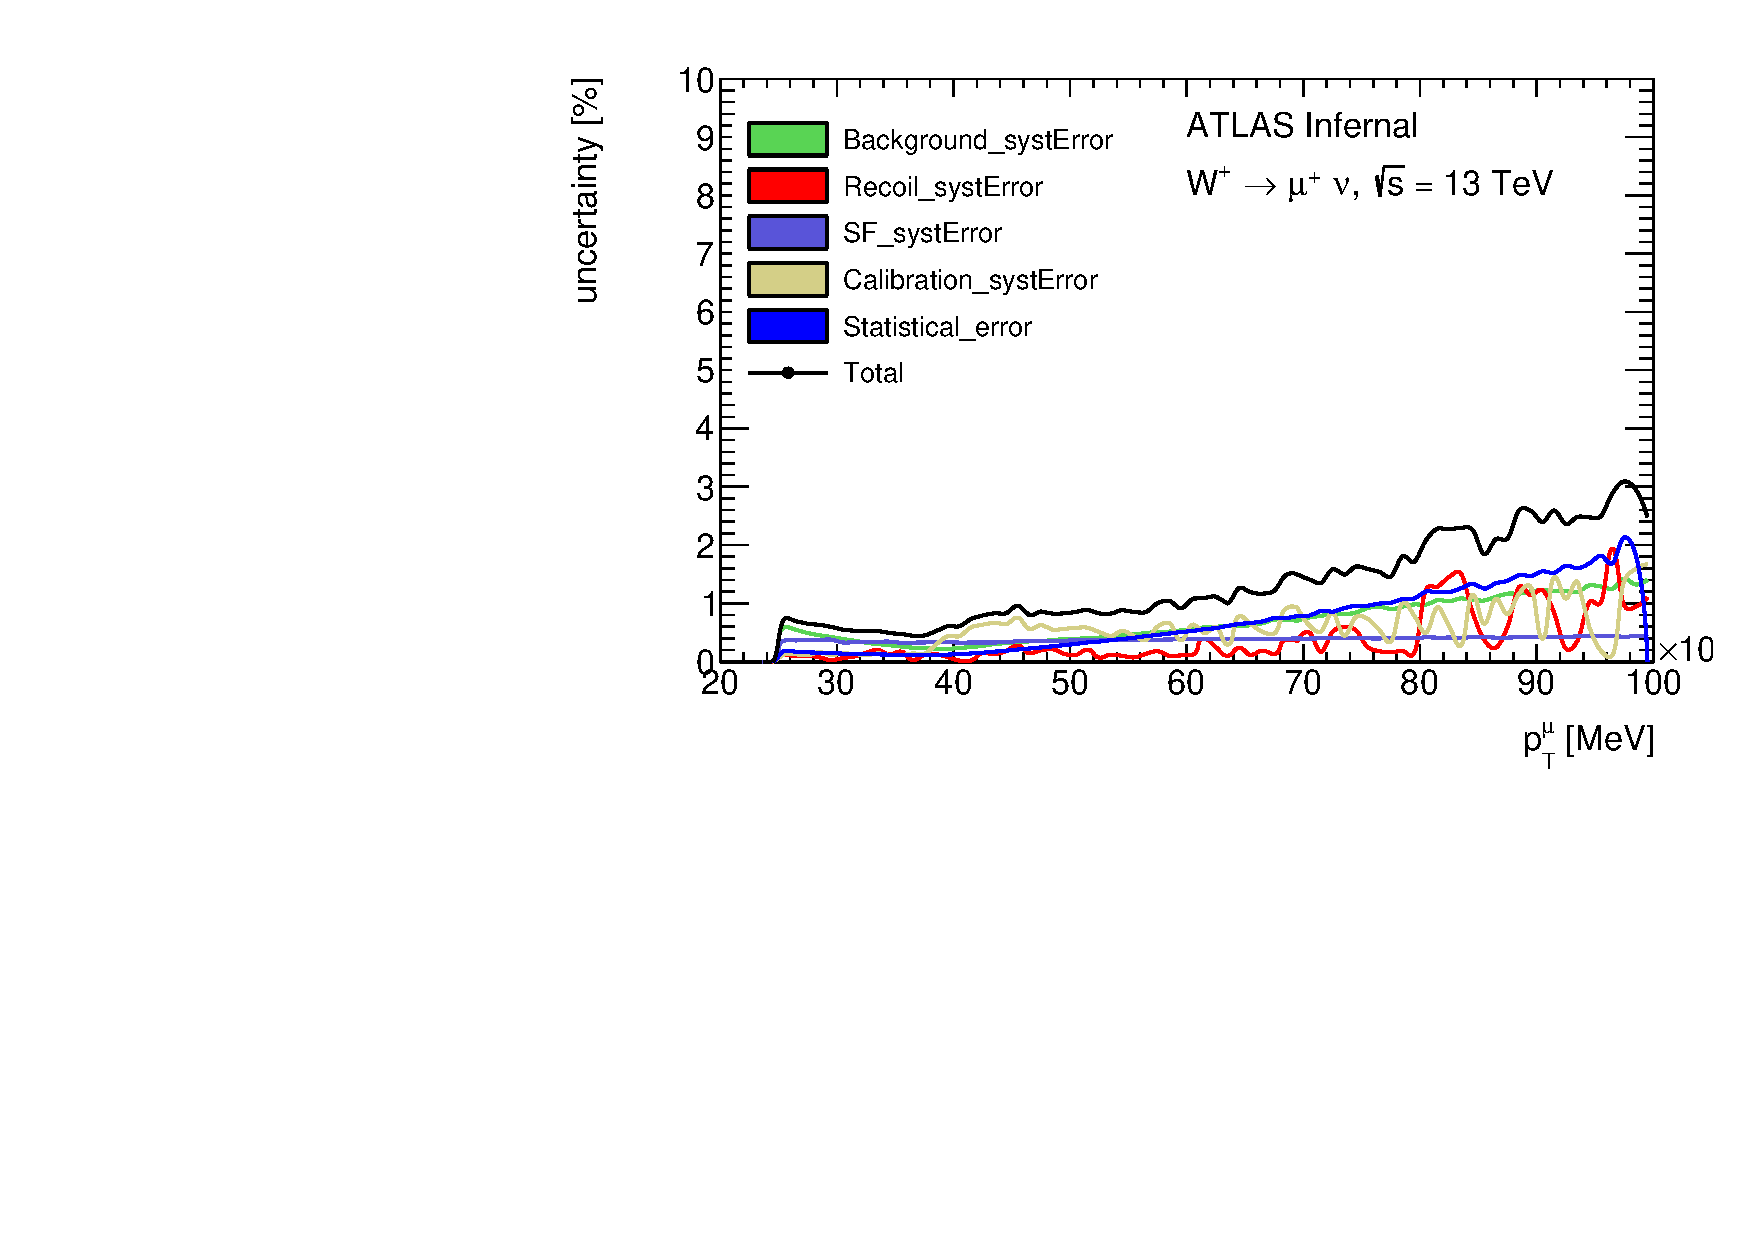
\includegraphics[width=.49\textwidth]{errors_muPt_cut7_plusmunu_13TeV__NormErr.pdf}\label{f:}}
	
	{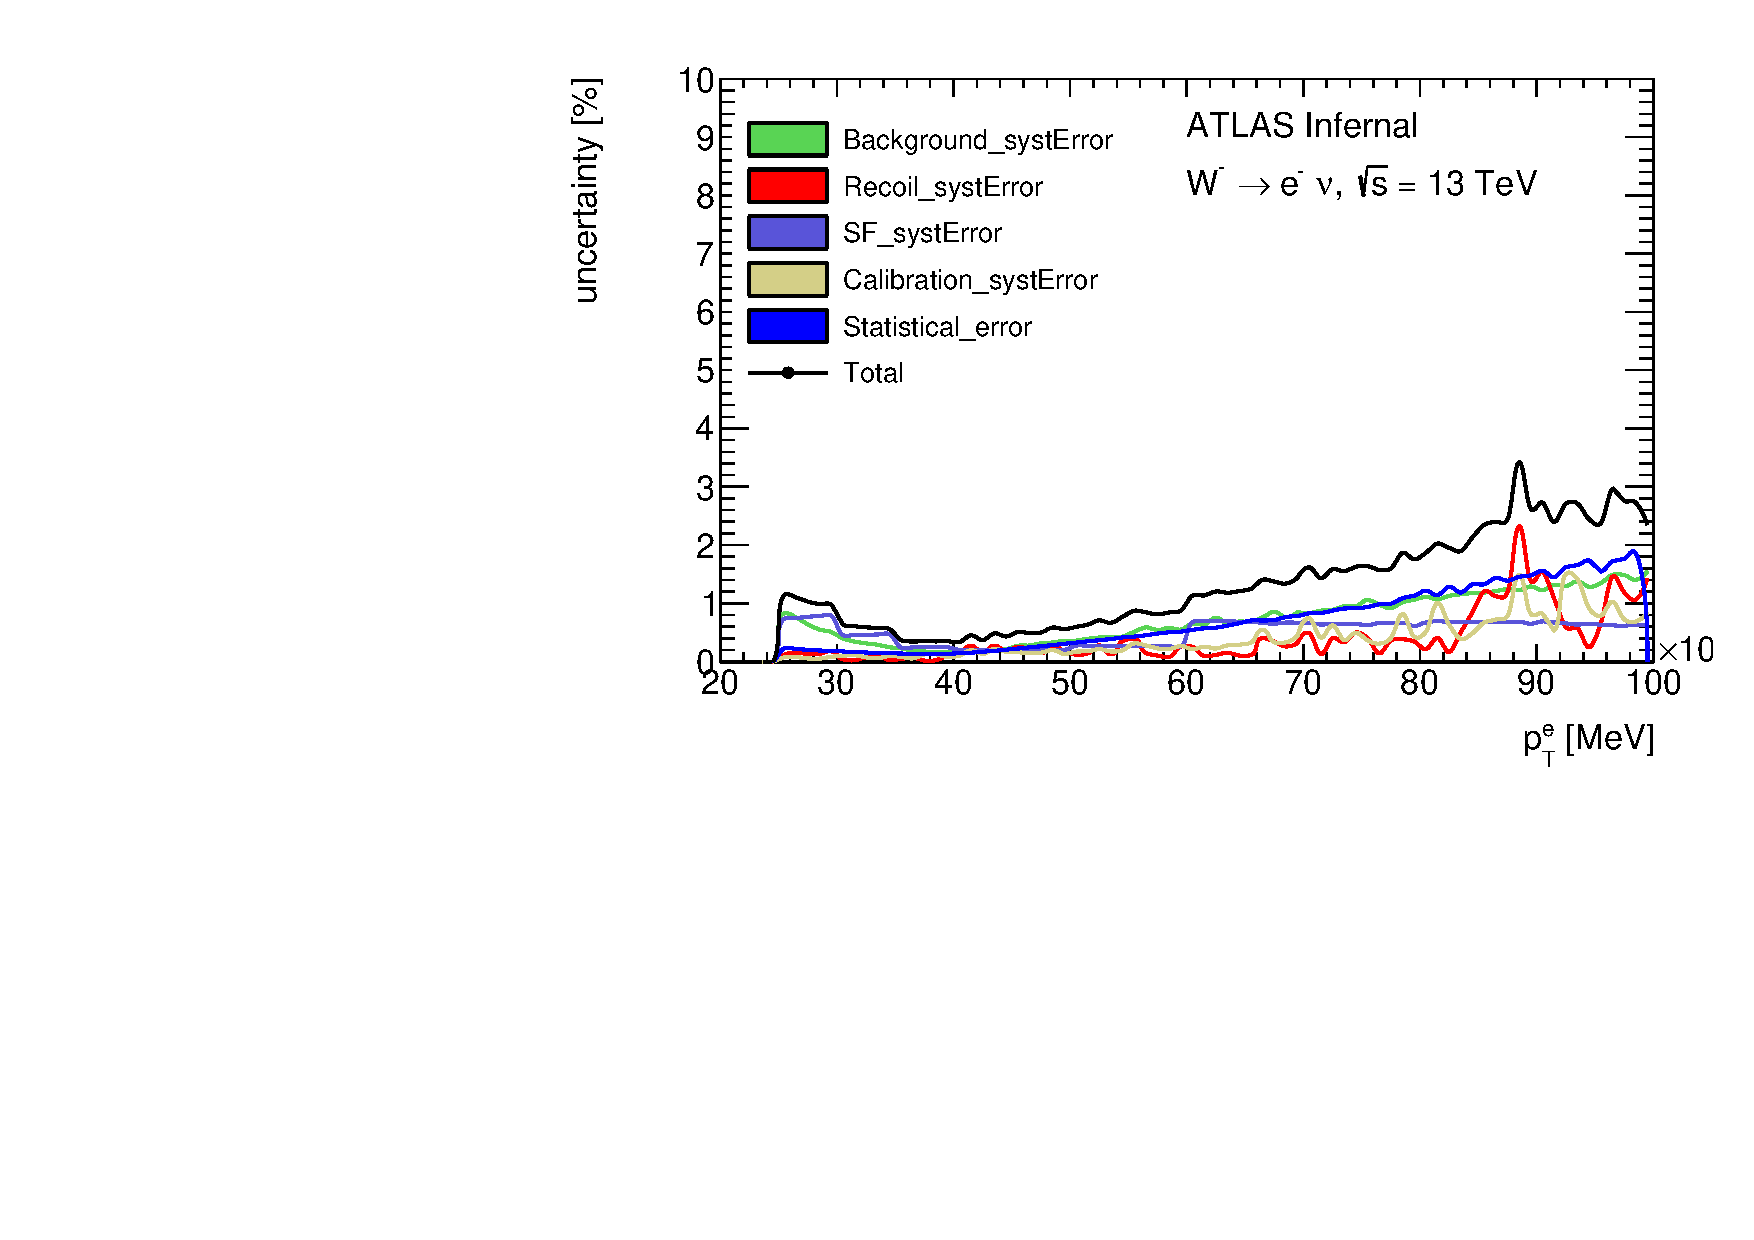
\includegraphics[width=.49\textwidth]{errors_elPt_cut7_minusenu_13TeV__NormErr.pdf}\label{f:}}
	{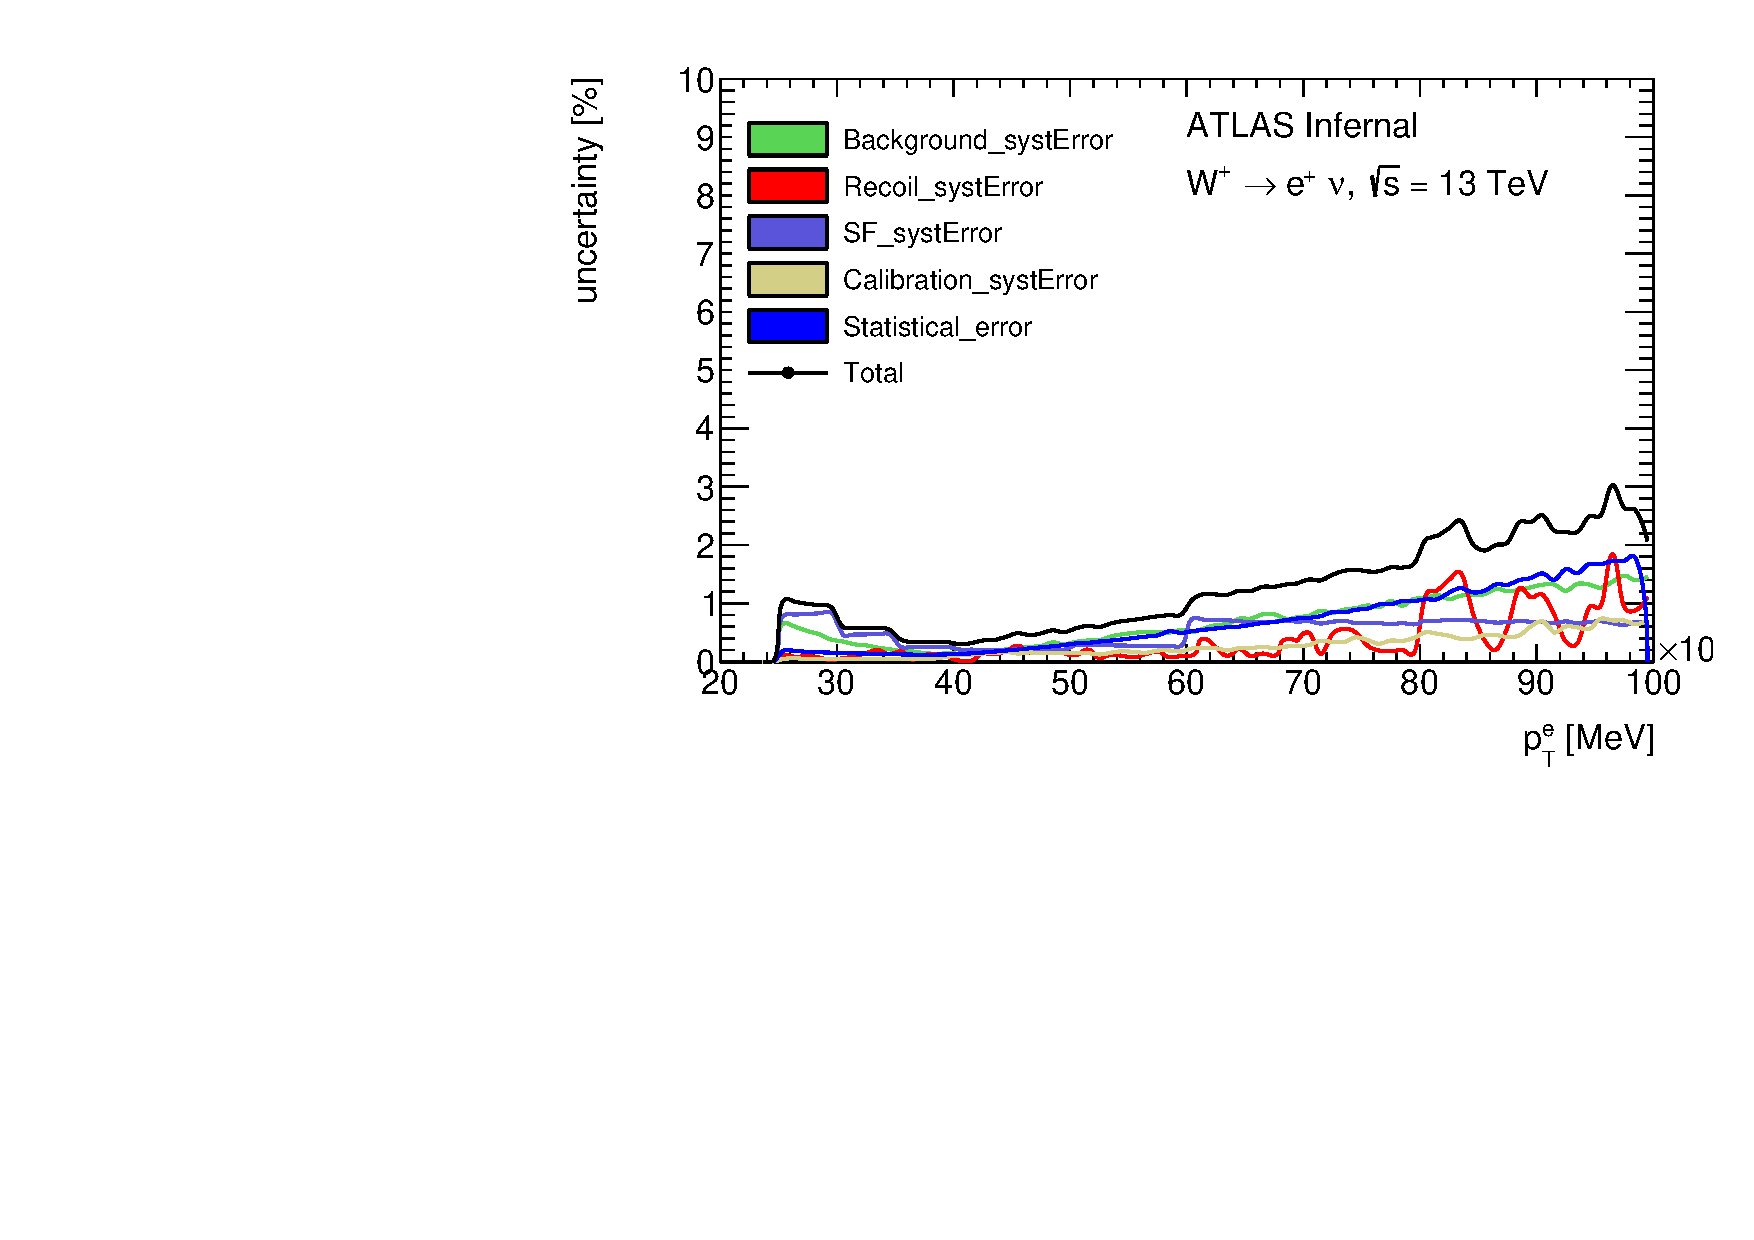
\includegraphics[width=.49\textwidth]{errors_elPt_cut7_plusenu_13TeV__NormErr.pdf}\label{f:}}
	\caption{  Lepton transverse systematic error breakdown distribution in the muon and electron channel  for the $\sqrt{s} = 5$~\TeV\ and $\sqrt{s} = 13$~\TeV\ datasets.}
\end{figure}
\newpage
\begin{figure}[h]
	\centering
	{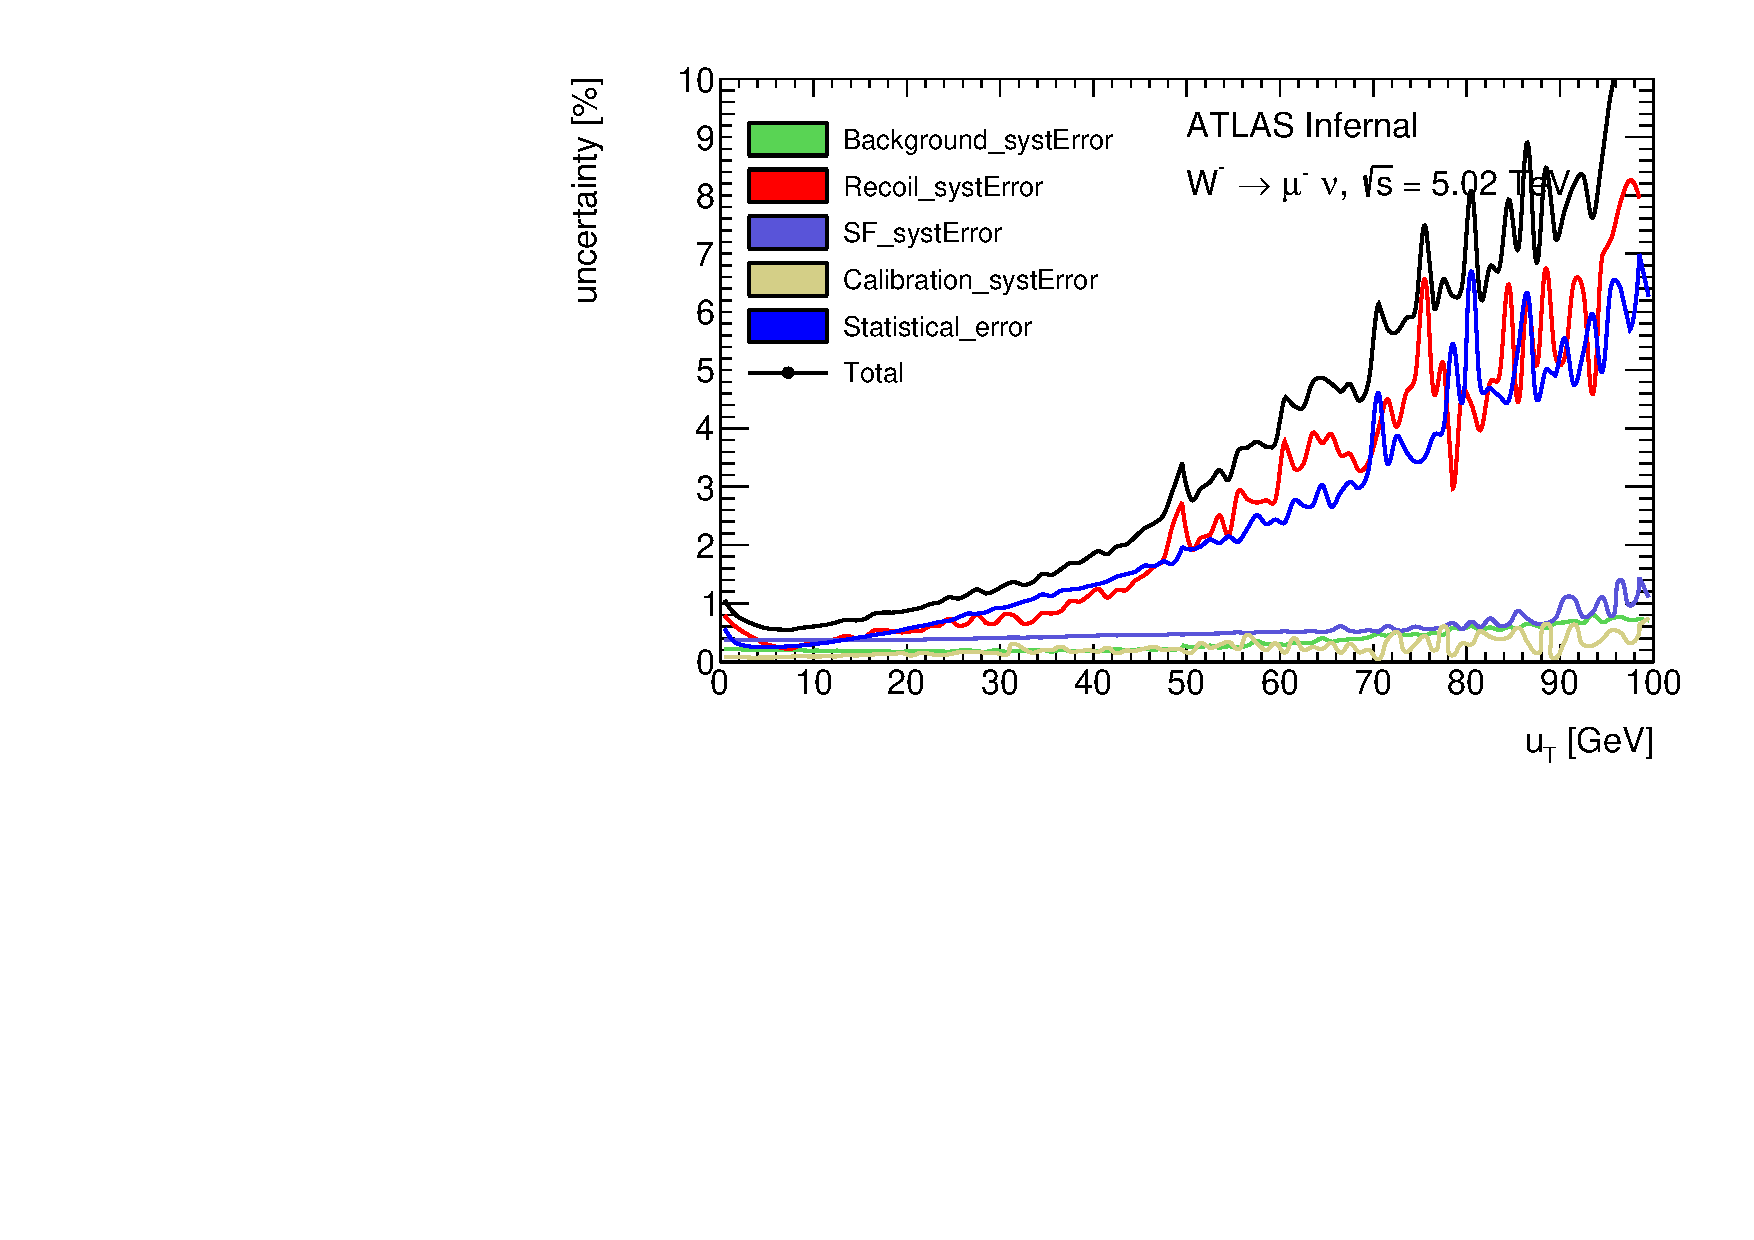
\includegraphics[width=.49\textwidth]{errors_WpT_Reco_cut7_minusmunu_5TeV__NormErr.pdf}\label{f:}}
	{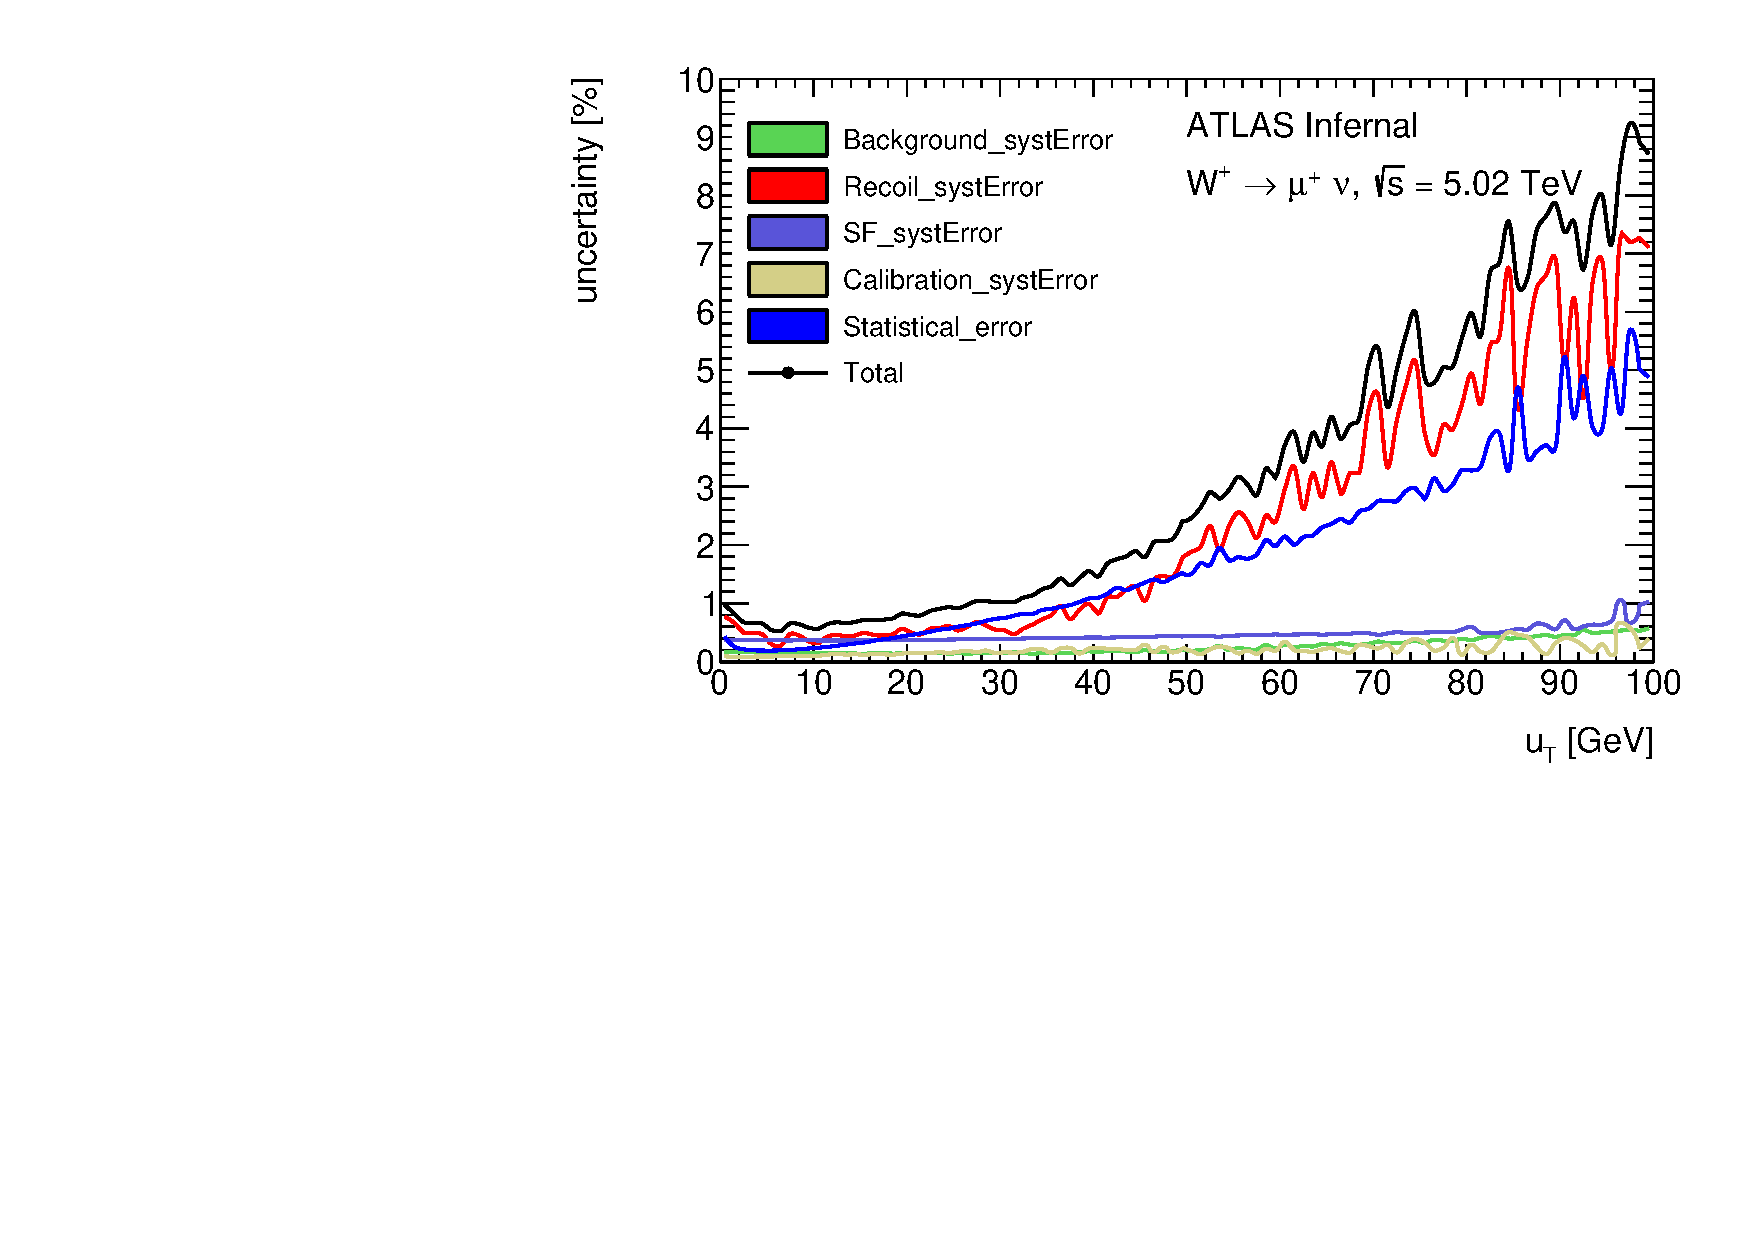
\includegraphics[width=.49\textwidth]{errors_WpT_Reco_cut7_plusmunu_5TeV__NormErr.pdf}\label{f:}}
	
	{\includegraphics[width=.49\textwidth]{errors_WpT_Reco_cut7_minusenu_5TeV__NormErr.pdf}\label{f:}}
	{\includegraphics[width=.49\textwidth]{errors_WpT_Reco_cut7_plusenu_5TeV__NormErr.pdf}\label{f:}}
	
		{\includegraphics[width=.49\textwidth]{errors_WpT_Reco_cut7_minusmunu_13TeV__NormErr.pdf}\label{f:}}
	{\includegraphics[width=.49\textwidth]{errors_WpT_Reco_cut7_plusmunu_13TeV__NormErr.pdf}\label{f:}}
	
	{\includegraphics[width=.49\textwidth]{errors_WpT_Reco_cut7_minusenu_13TeV__NormErr.pdf}\label{f:}}
	{\includegraphics[width=.49\textwidth]{errors_WpT_Reco_cut7_plusenu_13TeV__NormErr.pdf}\label{f:}}
	\caption{  W transverse momentum systematic error breakdown in the muon and electron channel  for the $\sqrt{s} = 5$~\TeV\ and $\sqrt{s} = 13$~\TeV\ datasets.}
\end{figure}
\newpage
\clearpage

